%% Rezolvari Fizica Moleculara si Termodinamica %%

\section*{2. FIZICĂ MOLECULARĂ ŞI TERMODINAMICĂ}

2.1 Masa molară a amestecului este: $\mu_{a}=\frac{m_{\mathrm{H}}+m_{\mathrm{CO}_{2}}}{\nu}$;\\ Numărul de moli de amestec este: $\nu=\nu_{1}+\nu_{2}=\frac{m_{\mathrm{H}}}{\mu_{\mathrm{H}}}+\frac{m_{\mathrm{CO}_{2}}}{\mu_{\mathrm{CO}_{2}}}$;\\ Deci: $\mu_{a}=\frac{m_{\mathrm{H}}+m_{\mathrm{CO}_{2}}}{\frac{m_{\mathrm{H}}}{\mu_{\mathrm{H}}}+\frac{m_{\mathrm{CO}_{2}}}{\mu_{\mathrm{CO}_{2}}}}=\mu_{\mathrm{H}} \mu_{\mathrm{CO}_{2}} \frac{m_{\mathrm{H}}+m_{\mathrm{CO}_{2}}}{m_{\mathrm{H}} \mu_{\mathrm{CO}_{2}}+m_{\mathrm{CO}_{2}} \mu_{\mathrm{H}}}=5,5 \cdot 10^{-3} \mathrm{~kg} / \mathrm{mol}$.\\

2.2 Transformăm Celsius în Kelvin:\\ $T_{1}=273+227=500 \mathrm{~K}; \quad T_{2}=273+27=300 \mathrm{~K}$.\\ Deci: $\frac{T_{1}-T_{2}}{T_{1}}=\frac{Q_{1}-\left|Q_{2}\right|}{Q_{1}}\left|Q_{2}\right|=Q_{1} \frac{T_{2}}{T_{1}}=1500 \mathrm{~J}$.\\

2.3. $Q=\nu C_{V}\left(T_{1}-T_{2}\right)$, unde $T_{1}=\frac{p_{1} V}{\nu R}$; $T_{2}=\frac{p_{2} V}{\nu R}$;\\ Deci: $Q=\nu \frac{5}{2} R V \frac{1}{\nu R}\left(p_{1}-p_{2}\right)=\frac{5}{2} V\left(p_{1}-p_{2}\right)$;\\ Obținem: $p_{2}=p_{1}-\frac{2}{5} \frac{Q}{V}=10^{5} \mathrm{~N} / \mathrm{m}^{2}$.\\

2.4. $Q=c_{p} m \Delta T=16,64 \mathrm{~kJ}$.

2.5. $L=p_{1}\left(V_{1}-V_{1}\right)+p_{2}\left(V_{2}-V_{1}\right)=p_{2}\left(\frac{p_{1} V_{1}}{p_{2}}-V_{1}\right)=V_{1}\left(p_{1}-p_{2}\right)=375 \mathrm{~J}$.\\

2.6. $\Delta U=\nu C_{V} \Delta T=\nu C_{V}\left(T_{3}-T_{1}\right)=\nu \frac{5}{2} R\left(\frac{p_{3} V_{2}}{v R}-\frac{p_{1} V_{1}}{v R}\right)= \\ =\frac{5}{2}\left(p_{3} V_{2}-p_{1} V_{1}\right)=6,5 \cdot 10^{6} \mathrm{~J}$.\\

2.7. Vitezele moleculelor la cele două temperaturi sunt:\\ $v_{T_{1}}=\sqrt{\frac{3 R T}{\mu}}$; \quad $v_{T_{2}}=\sqrt{\frac{3 R(T+\Delta T)}{\mu}}$;\\ Masa molară a gazului este: $\mu=\frac{3 R \Delta T}{v_{T_{2}}^{2}-v_{T_{1}}^{2}}=28 \cdot 10^{-3} \mathrm{~kg} / \mathrm{mol}$.\\

2.8. $N=N_{A} \frac{V}{V_{\mu_{0}}}=2,7 \cdot 10^{25}$ molecule. $N$ nu depinde de natura gazului.\\

2.9. $\frac{N_{\mathrm{O}_{2}}}{m}=\frac{N_{A}}{\mu_{\mathrm{O}_{2}}} \Rightarrow N_{\mathrm{O}_{2}}=m \frac{N_{A}}{\mu_{\mathrm{O}_{2}}}=3,765 \cdot 10^{25}$ molecule.\\

2.10. Ne folosim de relațiile: $p=n k_{B} T; \quad v_{T}^{2}=\frac{3 R T}{\mu}$;\\ Deci: $n=\frac{p}{k_{B} T}=\frac{3 p R}{k_{B} \mu v_{T}^{2}}=\frac{3 p N_{A}}{\mu v_{T}^{2}}=10^{25} \mathrm{~m}^{-3}$\\

2.11. Ne folosim de relațiile: $p=n k_{B} T; \quad n_{V}=n V$;\\ Deci: $n_{V}=\frac{p}{k_{B} T} V=\frac{p N_{A}}{R T} V \cong 2,68 \cdot 10^{3}$ molecule.\\

2.12. Scriem cele două ecuații de stare:\\ $\left.\begin{array}{l}p_{0} V_{0}=\nu R T_{0}\\ p V=\nu R T\end{array}\right\} \Rightarrow V_{0}=\frac{p V}{T} \frac{T_{0}}{p_{0}}=568,75 \mathrm{~m}^{3}$.\\

2.13. Din ecuația de stare: $p V=\nu R T=\frac{m}{\mu} R T \Rightarrow m=\frac{p V \mu}{R T}=16 \mathrm{~kg}$.\\

2.14. Scriem ecuațiile de stare, folosind densitatea:\\ $\left.\begin{array}{l}\rho=\frac{m}{V}=\frac{p \mu}{R T}\\ \rho_{0}=\frac{p_{0} \mu}{R T_{0}}\end{array}\right\} \Rightarrow \rho=\rho_{0} \frac{p}{p_{0}} \frac{T_{0}}{T}$.\\

2.15. Având de a face cu o transformare izotermă ($T=$ const.) şi masa fiind constantă ($m=$ const.), avem:\\ $p_{1} V_{1}=p_{2} V_{2}$, unde $p_{1}=p_{0}$, $V_{1}=S d_{1}$.\\ Presiunea $p_{2}$ rezultă din condiția:\\ $p_{2}=p_{0}+\frac{F}{S}$, $F$ fiind forța ce acționează asupra sistemului şi $V_{2}=S d_{2}$.\\ Astfel, se obține: $p_{0} S d_{1}=\left(p_{0}+\frac{F}{S}\right) S d_{2}$, de unde rezultă:\\ $F=S p_{0}\left(\frac{d_{1}}{d_{2}}-1\right)=1,25 \mathrm{~kN}$.\\

2.16. Transformăm Celsius în Kelvin:\\ $T_{1}=27+273=300 \mathrm{~K}; \quad T_{2}=47+273=320 \mathrm{~K}$.\\ Scriem ecuațiile de stare:\\ $\left.\begin{array}{l} p_{1} V=\frac{m_{1}}{\mu} R T_{1}\\ p_{2} V=\frac{m_{2}}{\mu} R T_{2} \end{array}\right\} \Rightarrow m=m_{2}-m_{1}=\frac{\mu V}{R}\left(\frac{p_{2}}{T_{2}}-\frac{p_{1}}{T_{1}}\right)=4,75 \cdot 10^{-2} \mathrm{~kg}$.\\

2.17. Transformăm Celsius în Kelvin:\\ $T_{1}=167+273=440 \mathrm{~K}; \quad T_{2}=255+273=528 \mathrm{~K}$.\\ Scriem ecuațiile de stare inițiale:\\ $\left.\begin{array}{l} p_{1} V=\nu_{1} R T_{1}\\ p_{2} V=\nu_{2} R T_{2} \end{array}\right\} \Rightarrow \frac{V_{1}}{V_{2}}=\frac{\nu_{1}}{\nu_{2}} \frac{T_{1}}{T_{2}} \Rightarrow \frac{\nu_{1}}{\nu_{2}}=\frac{V_{1} T_{2}}{V_{2} T_{1}}$\\ Scriem ecuațiile de stare după aducerea la aceeaşi temperatură:\\ $\left.\begin{array}{l} p^{\prime} V_{1}^{\prime}=\nu_{1} R T\\ p^{\prime} V_{2}^{\prime}=\nu_{2} R T \end{array}\right\} \Rightarrow \frac{V_{1}^{\prime}}{V_{2}^{\prime}}=\frac{\nu_{1}}{\nu_{2}}=\frac{V_{1} T_{2}}{V_{2} T_{1}}=0,8 \cdot \frac{528}{440}=0,96$.\\

2.18. Din ecuația de stare, avem:\\ $\rho_{0}=\frac{\mu p_{0}}{R T_{0}} \Rightarrow \frac{R}{\mu}=\frac{p_{0}}{\rho_{0} T_{0}}$.\\ Utilizând relația lui Mayer $c_{p}-c_{V}=\frac{R}{\mu}$, şi definiția lui $\gamma=\frac{c_{p}}{c_{V}}$, obţinem:\\ $c_{V}=\frac{p_{0}}{\rho_{0} T_{0}(\gamma-1)}=\frac{101325}{1,293 \cdot 273(1,41-1)}=700 \mathrm{~J} / \mathrm{kg} \cdot \mathrm{~K}$.\\ $c_{p}=\gamma \cdot c_{V}=1,41 \cdot 700=987 \mathrm{~J} / \mathrm{kg} \cdot \mathrm{~K}$.\\

2.19. Din relația lui Robert Mayer, $c_{p}-c_{V}=R / \mu$, rezultă:\\ $\mu=\frac{R}{c_{p}-c_{V}}=\frac{N_{A} k_{B}}{c_{p}-c_{V}}=4,14 \cdot 10^{-3} \mathrm{~kg} \cdot \mathrm{mol}^{-1}$.\\

2.20. La trecerea din starea inițială în cea finală, variația energiei interne este:\\ $\Delta U=v C_{V} \Delta T=\frac{m}{\mu} C_{V}\left(T_{3}-T_{1}\right)=\frac{5}{2} \frac{m}{\mu} R\left(T_{3}-T_{1}\right)$;\\ Ecuația de stare $p V=\frac{m}{\mu} R T$, ne permite sã obținem:\\ $T_{1}=\frac{\mu}{m} \frac{p_{1} V_{1}}{R} \text { şi } T_{3}=\frac{\mu}{m} \frac{p_{3} V_{2}}{R}$;\\ Astfel, variația energiei interne a gazului este:\\ $\Delta U=\frac{5}{2}\left(p_{3} V_{2}-p_{1} V_{1}\right)=3,45 \mathrm{~MJ}$.\\

2.21. Folosim două moduri de a scrie formula randamentului:\\ $\eta=\frac{L}{Q_{1}} \Rightarrow Q_{1}=\frac{L}{\eta}=\frac{400}{0,1}=4000 \mathrm{~J}$;\\ $\eta=\frac{Q_{1}-\left|Q_{2}\right|}{Q_{1}} \Rightarrow\left|Q_{2}\right|=Q_{1}(1-\eta)=4000(1-0,1)=3600 \mathrm{~J}$;\\ Căldura cedată la sursa rece este: $Q_{2}=-3600 \mathrm{~J}$.\\

2.22. Gazul se află în condiții normale dacă temperatura este $0^{\circ} \mathrm{C}$ şi presiunea este $1 \mathrm{~atm}$.\\

2.23. Numărul de molecule dintr-un mol de substanță se numeşte numărul lui Avogadro şi are valoarea $N_{A}=6,023 \cdot 10^{23}$ molecule $/ \mathrm{~mol}$.\\

2.24. Avogadro a formulat legea care îi poartă numele: volume egale de gaze diferite, aflate în aceleaşi condiții de temperatură şi presiune, au acelaşi număr de molecule.\\

2.25. Se numeşte mol cantitatea de substanță a cărei masă, exprimată în grame, este numeric egală cu masa moleculară relativă a substanței date.\\

2.26. $N=\nu \cdot N_{A}=\frac{m}{\mu} N_{A}=\frac{10^{3}}{18} \cdot 6,023 \cdot 10^{23} \text { molecule} / \mathrm{mol}= 3,346 \cdot 10^{25}$ molecule.\\

2.27. Energia internă a gazului ideal este funcție numai de temperatură, $U=U(T)$.\\

2.28. Energia internă a unui mol de gaz ideal monoatomic este: $U=3 R T / 2$.\\

2.29. Presiunea unui gaz ideal este legată de temperatură prin relația: $p=n k T$. Deci, concentrația moleculelor este: $n=\frac{p}{k T}=2,26 \cdot 10^{16} \mathrm{~m}^{-3}$.\\

2.30. Valoarea constantei universale, $R$, se exprimă în funcție de parametrii de stare $p_{0}=1 \mathrm{~atm}=1,013 \cdot 10^{5} \mathrm{~N} / \mathrm{m}^{2}$, $T_{0}=273,15 \mathrm{~K}$ şi $V_{\mu_{0}}=22,42 \mathrm{~m}^{3} / \mathrm{kmol}$, prin relația: $R=\frac{p_{0} V_{\mu_{0}}}{T_{0}}=8,31 \mathrm{~J} / \mathrm{mol} \cdot \mathrm{K}$.\\

2.31. Mărimea fizică numeric egală cu căldura necesară pentru a varia temperatura unui corp cu un grad se numeşte capacitate calorică a corpului și se notează, de obicei, prin $C$. Valoarea sa este dată de expresia: $C=\frac{Q}{\Delta T}$.\\ Se numeşte căldură specifică şi se notează cu $c$, căldura necesară pentru a varia temperatura unității de masă dintr-un corp cu un grad. Dacă masa corpului este $m$, atunci căldura specifică are expresia: $c=\frac{Q}{m \Delta T}$.\\

2.32. Din relația lui Robert Mayer: $C_{p}-C_{V}=R$, iar din definiția lui $\gamma$ avem: $\frac{C_{p}}{C_{V}}=\gamma$. Dacă rezolvăm sistemul de ecuații de mai sus, obținem:\\ $C_{V}=\frac{R}{\gamma-1}=\frac{8,31}{1,41-1}=20,27 \mathrm{~J} / \mathrm{mol} \cdot \mathrm{K}$;\\ $C_{p}=\frac{\gamma R}{\gamma-1}=\gamma C_{V}=28,58 \mathrm{~J} / \mathrm{mol} \cdot \mathrm{K}$.\\

2.33. Într-o transformare izotermă, un mol de gaz execută un lucru mecanic:\\ $L=2,3 R T \lg \frac{V_{2}}{V_{1}}$.\\

2.34. $Q=m c\left(t_{2}-t_{1}\right)=2 \cdot 4200 \cdot 60 \mathrm{~J}=504 \mathrm{~kJ}$.\\

2.35. $Q=m c \Delta t=10 \cdot 500 \cdot 10=5 \cdot 10^{4} \mathrm{~J}$.\\

2.36. Din ecuaţia de stare, avem: $p V=\frac{m}{\mu} R T \Rightarrow \rho=\frac{m}{V}=\frac{p \mu}{R T}$.\\ Deci: $\rho=\frac{1,013 \cdot 10^{5} \cdot 29 \cdot 10^{-3}}{8,31 \cdot 300}=1,18 \mathrm{~kg} / \mathrm{m}^{3}$.\\

2.37. Gazul este supus unei transformări izobare de la starea $\left(V_{0}, T_{0}\right)$ la starea $\left(2 V_{0}, T_{0}\right)$. Deci:\\ $\frac{V_{0}}{T_{0}}=\frac{2 V_{0}}{T} \Rightarrow T=2 T_{0}=2 \cdot 273=546 \mathrm{~K} \text { şi } t=T-273=273^{\circ} \mathrm{C}$.\\

2.38. Randamentul compresorului este $\eta=\frac{P_{u}}{P_{c}}$ unde $P_{u}$ este puterea utilă a compresorului, iar $P_{c}$ este puterea sa consumată, care reprezintă puterea utilă a motorului. Energia care este transformată în căldură în timpul $t$ este:\\ $W=\left(P_{c}-P_{u}\right) \cdot t=P_{c}(1-\eta) \cdot t$;\\ Această căldură este cea care încălzeşte apa de răcire cu $\Delta t$. Deci:\\ $m c \Delta t=\rho V c \Delta t=P_{c}(1-\eta) \cdot t \Rightarrow P_{c}=\frac{\rho V c \Delta t}{(1-\eta) \cdot t}=31,5 \mathrm{~kW}$.\\

2.39. Prin definiție, randamentul este: $\eta=\frac{Q_{1}-\left|Q_{2}\right|}{Q_{1}}=1-\frac{\left|Q_{2}\right|}{Q_{1}} \quad (1)$\\ Motorul primeşte căldura $Q_{1}$ în procesul izocor $2 \rightarrow 3$ şi cedează căldura $Q_{2}$ în procesul izocor $4 \rightarrow 1$ (vezi figura problemei).\\ Deci: $Q_{1}=\nu C_{V}\left(T_{3}-T_{2}\right)$ şi $\left|Q_{2}\right|=\nu C_{V}\left(T_{4}-T_{1}\right) \quad (2)$\\ Înlocuim (2) în (1) şi obținem: $\eta=1-\frac{T_{4}-T_{1}}{T_{3}-T_{2}} \quad (3)$\\ Stările 1 şi 2 se găsesc pe aceeaşi adiabată şi putem scrie:\\ $T_{1} V_{1}^{\gamma-1}=T_{2} V_{2}^{\gamma-1}$, de unde $T_{2}=T_{1} \varepsilon^{\gamma-1} \quad (4)$\\ Stările 3 şi 4 se găsesc pe adiabata de sus, şi rezultă:\\ $T_{3} V_{3}^{\gamma-1}=T_{4} V_{4}^{\gamma-1}$ sau $\frac{T_{3}}{T_{4}}=\left(\frac{V_{4}}{V_{3}}\right)^{\gamma-1} \quad (5)$\\ Cum $V_{4}=V_{1}$ şi $V_{3}=V_{2}$ rezultă: $T_{3}=T_{4} \varepsilon^{\gamma-1}$\\ Înlocuim (4) şi (5) în (3) şi obținem randamentul:\\ $\eta=1-\frac{1}{\varepsilon^{\gamma-1}}=1-\frac{1}{3}=0,66$.\\ \begin{center} 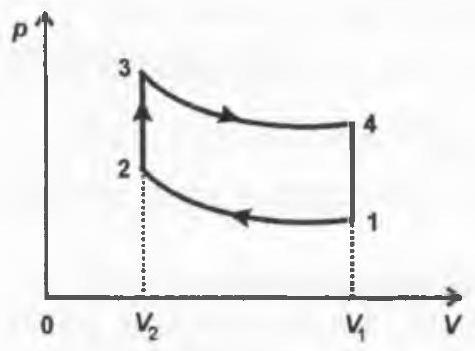
\includegraphics[max width=\textwidth, center]{2025_07_01_5b3ff9fa0d508c8e9f17g-276}\\ Figura problemei \end{center}\\

2.40. Avem: $V_{2}=V_{1} / n$; \quad $V_{2}^{\gamma} p_{2}=p_{1} V_{1}^{\gamma}$, deci $p_{2}=p_{1}\left(\frac{V_{1}}{V_{2}}\right)^{\gamma}=n^{\gamma} p_{1}$.\\ $T_{2}=T_{1}\left(\frac{V_{1}}{V_{2}}\right)^{\gamma-1}=T_{1} n^{\gamma-1}$; \quad $T_{3}=\frac{V_{3}}{V_{2}} T_{2}=k T_{2}=k n^{\gamma-1} T_{1}$;\\ $V_{4}=V_{1}$; \quad $p_{4}=p_{2}\left(\frac{V_{3}}{V_{1}}\right)^{\gamma}=p_{2}\left(\frac{V_{3}}{V_{2}} \frac{V_{2}}{V_{1}}\right)^{\gamma}=p_{2}\left(\frac{k}{n}\right)^{\gamma}$;\\ $T_{4}=T_{3}\left(\frac{V_{3}}{V_{1}}\right)^{\gamma-1}=T_{3}\left(\frac{k}{n}\right)^{\gamma-1}=k n^{\gamma-1}\left(\frac{k}{n}\right)^{\gamma-1} T_{1}=k^{\gamma} T_{1}$.\\ Randamentul ciclului este:\\ $\eta=1-\frac{\left|Q_{2}\right|}{Q_{1}}=1-\frac{\nu C_{V}\left(T_{4}-T_{1}\right)}{\nu C_{p}\left(T_{3}-T_{2}\right)}=1-\frac{1}{\gamma} \frac{T_{4}-T_{1}}{T_{3}-T_{2}}$.\\ Exprimăm $T_{2}$, $T_{3}$ şi $T_{4}$ în funcție de $T_{1}$:\\ $T_{2}=T_{1} n^{\gamma-1}$; $T_{3}=k n^{\gamma-1} T_{1}$ şi $T_{4}=k^{\gamma} T_{1}$.\\ Introducem în expresia randamentului şi obținem:\\ $\eta=1-\frac{1}{\gamma} \frac{k^{\gamma}-1}{n^{\gamma-1}(k-1)}=1-\frac{1}{1,4} \cdot \frac{2,64-1}{2,51 \cdot(2-1)}=0,54$.\\

2.41. $\bar{E}=N \bar{\varepsilon}_{t r}=N \cdot \frac{3}{2} k T \Rightarrow N=\frac{2 \bar{E}}{3 k T}=\frac{2 \cdot 6,2}{3 \cdot 1,38 \cdot 10^{-23} \cdot 300}=10^{21}$ particule.\\

2.42. În transformările izoterme $2 \rightarrow 3$ şi $4 \rightarrow 1$, energia internă nu se schimbă și din principiul I al termodinamicii rezultă:\\ $Q_{23}=L_{23}=\nu R T_{2} \ln \frac{V_{3}}{V_{2}}>0$;\\ $Q_{41}=L_{41}=\nu R T_{1} \ln \frac{V_{1}}{V_{4}}<0$;\\ În transformările $1 \rightarrow 2$ şi $3 \rightarrow 4$ căldurile $Q_{12}$ şi $Q_{34}$ sunt:\\ $Q_{12}=\nu C\left(T_{2}-T_{1}\right)=\nu \cdot 2 R\left(T_{2}-T_{1}\right)>0$;\\ $Q_{34}=\nu C\left(T_{1}-T_{2}\right)=\nu \cdot 2 R\left(T_{1}-T_{2}\right)<0$;\\ Prin urmare, căldura absorbită este:\\ $Q_{abs}=Q_{12}+Q_{23}=\nu \cdot 2 R\left(T_{2}-T_{1}\right)+\nu R T_{2} \ln \frac{V_{3}}{V_{2}}$.\\ Căldura cedată (în modul) este:\\ $\left|Q_{ced}\right|=\left|Q_{34}\right|+\left|Q_{41}\right|=\nu \cdot 2 R\left(T_{2}-T_{1}\right)+\nu R T_{1} \ln \frac{V_{4}}{V_{1}}$.\\ Lucrul efectuat într-un ciclu:\\ $L=Q_{abs}-\left|Q_{ced}\right|=\nu R T_{2} \ln \frac{V_{3}}{V_{2}}-\nu R T_{1} \ln \frac{V_{4}}{V_{1}}$.\\ Randamentul ciclului este:\\ $\eta=\frac{L}{Q_{abs}}=\frac{\nu R T_{2} \ln \frac{V_{3}}{V_{2}}-\nu R T_{1} \ln \frac{V_{4}}{V_{1}}}{\nu \cdot 2 R\left(T_{2}-T_{1}\right)+\nu R T_{2} \ln \frac{V_{3}}{V_{2}}}$.\\ Pentru transformările liniare $1 \rightarrow 2$ şi $3 \rightarrow 4$ avem relațiile:\\ $p_{1}=V_{1} \operatorname{tg} 2 \alpha$; \quad $p_{2}=V_{2} \operatorname{tg} 2 \alpha$;\\ $p_{3}=V_{3} \operatorname{tg} \alpha$; \quad $p_{4}=V_{4} \operatorname{tg} \alpha$.\\ Dacă în relațiile de mai sus utilizăm ecuația de stare $p V=\nu R T$ obținem: $\nu R T_{1}=V_{1}^{2} \operatorname{tg} 2 \alpha$, $\nu R T_{2}=V_{2}^{2} \operatorname{tg} 2 \alpha$ şi $\nu R T_{3}=V_{3}^{2} \operatorname{tg} \alpha$. Din acestea aflăm rapoartele: $V_{3} / V_{2}$ şi $V_{4} / V_{1}$ pe care le introducem în expresia randamentului pentru a obține:\\ $\eta=\frac{1}{2} \ln \frac{\operatorname{tg} 2 \alpha}{\operatorname{tg} \alpha} \cdot \frac{T_{2}-T_{1}}{2\left(T_{2}-T_{1}\right)+\frac{1}{2} T_{2} \ln \frac{\operatorname{tg} 2 \alpha}{\operatorname{tg} \alpha}}=0,15$.\\

2.43. Gazul din compartimentul închis suferă o transformare izobară la presiunea atmosferică $p_{0}$. Volumul său inițial este $V_{0}=L S$ unde $S$ este secțiunea cilindrului. Volumul final este $V_{1}=1,25 L S$. Din legea transformării izobare avem:\\ $\frac{V_{0}}{V_{1}}=\frac{T_{0}}{T_{1}} \Rightarrow T_{1}=\frac{V_{1}}{V_{0}} T_{0}=1,25 T_{0} \quad (1)$\\ Căldura cedată de rezistența $R_{1}$ în timpul $\tau$ este: $Q=\frac{U^{2}}{R_{1}} \cdot \tau \quad (2)$\\ Din primul principiu al termodinamicii, avem:\\ $Q=\Delta U+p_{0} \Delta V=\frac{3}{2} \nu R\left(T_{1}-T_{0}\right)+\nu R\left(T_{1}-T_{0}\right) \quad (3)$\\ Din (2) şi (3) rezultă:\\ $R_{1}=\frac{U^{2} \tau}{\frac{5}{2} \nu R\left(T_{1}-T\right)}=\frac{U^{2} \tau}{\frac{5}{2} \cdot \frac{4}{R} R \cdot 0,25 T_{0}}=\frac{2 U^{2} \tau}{5 T_{0}}=8 \Omega$.\\

2.44. $\frac{\mu m g s}{2}=m c \Delta t \Rightarrow \Delta t=\frac{\mu g s}{2 c}=2$ grade.\\

2.45. Variația energiei interne a gazului ideal corespunzătoare unei variații de temperatură $\Delta T$ este $\Delta U=\nu C_{V} \Delta T$.\\ Avem relaţia lui Robert Mayer, $C_{p}-C_{V}=R$ sau $\gamma C_{V}-C_{V}=R$, de unde $C_{V}=\frac{R}{\gamma-1}$.\\ Deci: $\Delta U=\frac{1}{\gamma-1}\left(\nu R T_{2}-\nu R T_{1}\right)=\frac{1}{\gamma-1}\left(p_{2} V_{2}-p_{1} V_{1}\right)= \\ =\frac{1}{\gamma-1}\left(n^{2} p_{1} V_{1}-p_{1} V_{1}\right)=\frac{n^{2}-1}{\gamma-1} b V_{1}^{2}$.\\ \begin{center} 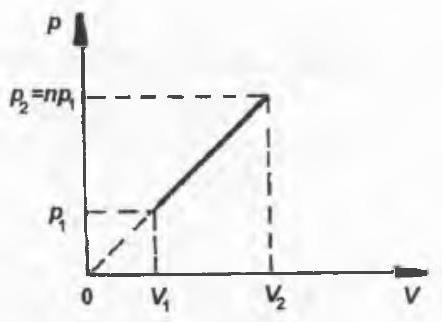
\includegraphics[max width=\textwidth]{2025_07_01_5b3ff9fa0d508c8e9f17g-279}\\ Figura problemei \end{center}\\

2.46. Din legea generală a gazelor, avem:\\ $p V=\frac{m}{\mu} R T \Rightarrow p \mu=\frac{m}{V} R T \Rightarrow \frac{p}{\rho}=\frac{R T}{\mu}$.\\ Raportul este constant când $T=$ const., deci în transformarea izotermă.\\

2.47. Ecuația calorimetrică se scrie:\\ $m_{1} c\left(t_{f}-t_{1}\right)+m_{2} c\left(t_{f}-t_{2}\right)+m_{3} c\left(t_{f}-t_{3}\right)=0$;\\ Rezultă: $t_{f}=\frac{m_{1} t_{1}+m_{2} t_{2}+m_{3} t_{3}}{m_{1}+m_{2}+m_{3}}=\frac{t_{1}+t_{2}+t_{3}}{3}=41^{\circ} \mathrm{C}$.\\

2.48. În transformarea izobară, $L=p_{1} \Delta V$.\\ Din legea gazelor, avem: $p_{1}=\frac{\nu R T_{1}}{V_{1}} \Rightarrow \Delta V=\frac{L V_{1}}{\nu R T_{1}}$.\\ La presiune constantă, $\frac{V_{2}}{T_{2}}=\frac{V_{1}}{T_{1}}$ sau $\frac{V_{2}-V_{1}}{T_{2}-T_{1}}=\frac{V_{1}}{T_{1}}$.\\ De aici: $T_{2}=T_{1}+\Delta V \frac{T_{1}}{V_{1}}=T_{1}+\frac{L}{\nu R}=510 \mathrm{~K}$.\\

2.49. Randamentul ciclului Carnot este: $\eta=1-\frac{T_{2}}{T_{1}}=\frac{2}{5}$.\\ În general, $\eta=\frac{L}{Q_{1}}=\frac{Q_{1}-Q_{2}}{Q_{1}}$.\\ Rezultă: $\eta L=L-\eta Q_{2} \Rightarrow Q_{2}=\frac{L(1-\eta)}{\eta}=\frac{3}{2} L=1,2 \cdot 10^{5} \mathrm{~J}$.\\

2.50. General vorbind, viteza termică este: $v_{t}=\sqrt{\frac{3 R T}{\mu}}=\sqrt{\frac{3 p V}{m}}=\sqrt{\frac{3 p}{\rho}}$.\\ Deci, în cazul nostru avem: $\frac{\left(v_{t}\right)_{2}}{\left(v_{t}\right)_{1}}=\frac{\sqrt{\frac{3 p_{2}}{\rho_{2}}}}{\sqrt{\frac{3 p_{1}}{\rho_{1}}}}=\sqrt{\frac{p_{2}}{p_{1}} \cdot \frac{\rho_{1}}{\rho_{2}}}=2$.\\

2.51. Avem: $v_{t}^{2}=\frac{3 R T}{\mu}$ şi $p=n \frac{R}{N_{A}} T$. Rezultă $v_{t}^{2}=\frac{3 p N_{A}}{n \mu}$, de unde:\\ $n=\frac{3 p N_{A}}{\mu v_{t}^{2}}=1,8 \cdot 10^{25} \text { molec} / \mathrm{m}^{3}$.\\

2.52. Scriem legea gazelor ideale: $p V=v R T$. Temperatura maximă este atinsă în starea 2, iar cea minimă în starea 1.\\ $p_{1} V_{1}=\nu R T^{\prime} \Rightarrow T^{\prime}=\frac{p_{1} V_{1}}{\nu R}$;\\ $p_{2} V_{2}=\nu R T^{\prime \prime} \Rightarrow T^{\prime \prime}=\frac{p_{2} V_{2}}{\nu R}$;\\ Deci: $\eta=1-\frac{T_{2}}{T_{1}}=1-\frac{T^{\prime}}{T^{\prime \prime}}=\frac{p_{1} V_{1}}{2 p_{1} 3 V_{1}}=\frac{1}{6}$.\\

2.53. Situația este arătată în figura problemei. Energia internă în stările inițială şi finală este:\\ $U_{1}=\frac{3}{2} \nu R T_{1}=\frac{3}{2} p_{1} V_{1}$;\\ $U_{2}=\frac{3}{2} \nu R T_{2}=\frac{3}{2} p_{2} V_{2}=\frac{3}{2} \frac{V_{1}}{n} p_{1} \frac{n}{2}=\frac{3}{4} p_{1} V_{1}=\frac{U_{1}}{2}$.\\ \begin{center} 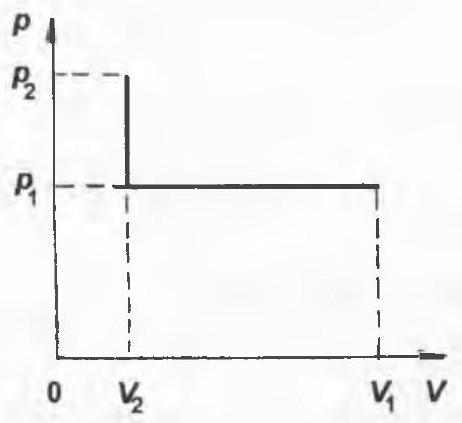
\includegraphics[max width=\textwidth, center]{2025_07_01_5b3ff9fa0d508c8e9f17g-281(1)}\\ Figura problemei \end{center}\\

2.54. Transformările sunt izobare $\frac{V}{T}=$ const. Din legea gazelor $\frac{V}{T}=\frac{\nu R}{p}$, rezultă $p_{2} \neq \frac{p_{1}+p_{3}}{2}$.\\

2.55. Gazul suferă o transformare izotermă:\\ $p=\frac{p_{0} V_{0}}{V}=\frac{p_{0} S L}{S\left(L-l^{\prime}\right)}$;\\ Din echilibrul presiunilor (vezi figura problemei):\\ $p=p_{0}+\rho g\left(l-l^{\prime}\right)$.\\ Din acestea rezultă:\\ $L=\frac{l^{\prime}\left[p_{0}+\rho g\left(l-l^{\prime}\right)\right]}{\rho g\left(l-l^{\prime}\right)}=\frac{0,06\left\lfloor 10^{5}+10^{3} \cdot 10(0,66-0,06)\right\rfloor}{10^{3} \cdot 10(0,66-0,06)}=1,06 \mathrm{~m}$.\\ \begin{center} 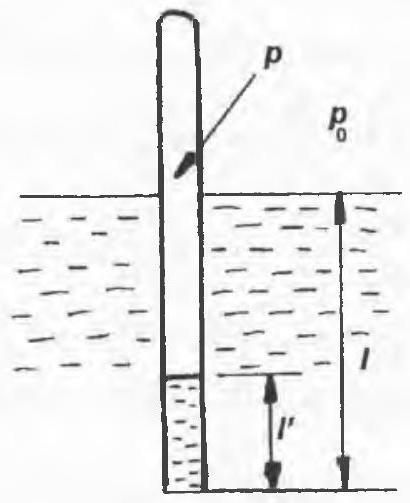
\includegraphics[max width=\textwidth, center]{2025_07_01_5b3ff9fa0d508c8e9f17g-281}\\ Figura problemei \end{center}\\

2.56. Scriem ecuațiile de stare şi relațiile dintre parametrii stărilor:\\ $p_{1} V=\frac{m_{1}}{\mu} R T_{1}$; \quad $p_{2} V=\frac{m_{2}}{\mu} R T_{2}$.\\ $p_{2}=p_{1}\left(1-f_{1}\right)$; \quad $T_{2}=T_{1}\left(1-f_{2}\right)$; \quad $m_{2}=m_{1}(1-f)$.\\ Rescriem a doua ecuație:\\ $p_{1}\left(1-f_{1}\right) V=\frac{m_{1}\left(1-f_{1}\right)}{\mu} R T_{1}\left(1-f_{2}\right)$, dar $p_{1} V=\frac{m_{1}}{\mu} R T_{1}$;\\ Deci: $\left(1-f_{1}\right)=(1-f)\left(1-f_{2}\right) \Rightarrow 1-f=\frac{1-f_{1}}{1-f_{2}} \Rightarrow f=1-\frac{1-f_{1}}{1-f_{2}}$;\\ $f=\frac{1-f_{2}-1+f_{1}}{1-f_{2}}=\frac{f_{1}-f_{2}}{1-f_{2}}=0,2 \Rightarrow f=20 \%$.\\

2.57. Avem $L=\frac{3 V \cdot p}{2}$.\\ $Q_{1}=\nu C_{V}\left(T_{2}-T_{1}\right)+\nu C_{p}\left(T_{3}-T_{2}\right)$;\\ Scriem legile transformărilor izobară şi izocoră:\\  $\frac{p_{2}}{p_{1}}=\frac{T_{2}}{T_{1}} \Rightarrow 2=\frac{T_{2}}{T_{1}} \Rightarrow T_{2}=2 T_{1}$;\\ $\frac{V_{3}}{V_{2}}=\frac{T_{3}}{T_{2}} \Rightarrow 4=\frac{T_{3}}{T_{2}} \Rightarrow T_{3}=4 T_{2}=8 T_{1}$;\\ Deci:\\ $Q_{1}=\nu C_{V}\left(2 T_{1}-T_{1}\right)+\nu C_{p}\left(8 T_{1}-2 T_{1}\right)$;\\ $Q_{1}=\nu C_{V} T_{1}+\nu\left(C_{V}+R\right) \cdot 6 T_{1}=7 \gamma C_{V} T_{1}+6 R \nu T_{1}$;\\ Randamentul este:\\ $\eta=\frac{3 p V}{2 v\left(7 C_{V} T_{1}+6 R T_{1}\right)}=\frac{3 p V}{2 v T_{1}\left(7 C_{V}+6 R\right)}$.\\ Dar $p V=v R T_{1} \Rightarrow \eta=\frac{3}{2} \frac{R}{7 C_{V}+6 R}$.\\ $\left\{\begin{array}{ll} C_{V}=C_{p}-R; \quad C_{p}=\gamma C_{V}\\ \frac{C_{p}}{C_{V}}=\gamma; \quad C_{V}=\frac{R}{\gamma-1}\\ \end{array}\right.$\\ Deci: $\eta=\frac{3}{2} \frac{R}{\frac{7 R}{\gamma-1}+6 R}=\frac{3}{2} \frac{R(\gamma-1)}{7 R+6 R(\gamma-1)}=\frac{3}{2} \frac{\gamma-1}{1+6 \gamma}$.\\

2.58. $p=n k T \Rightarrow n=\frac{p}{k T}=2,4 \cdot 10^{25} \mathrm{~m}^{-3}$.\\ Ecuații de stare: $p_{0} V=\nu R T_{1}$; \quad $p V=\nu R T_{2}$;\\ Dar $p S=m g+p_{0} S$\\ Deci: $T_{2}=\frac{p_{0} S+m g}{p_{0} S}=306 \mathrm{~K}$.\\

2.59. Din randamentul inițial, avem: $\eta=1-\frac{T_{2}}{T_{1}}$ sau $T_{1}=\frac{T_{2}}{1-\eta}$.\\ Pentru a doua situație, avem: $\eta^{\prime}=1-\frac{T_{2}^{\prime}}{T_{1}}=1-\frac{T_{2}-\Delta T}{T_{1}}$.\\ Variația temperaturii este: $\Delta T=T_{2}\left(1-\frac{1-\eta^{\prime}}{1-\eta}\right)=50 \mathrm{~K}$.\\ $P=\frac{L}{t}$, $\eta=\frac{L}{Q_{1}} \Rightarrow P=24 \mathrm{~kW}$.\\

2.60. $\left(\nu_{1}+\nu_{2}\right) C \Delta T=\left(\nu_{1} C_{V_{1}}+\nu_{2} C_{V_{2}}\right) \Delta T$;\\ Cum $\nu=\frac{N}{N_{A}}$, obţinem $C=\frac{11}{6} R$.\\

2.61. $p=\frac{2}{3} \frac{N}{V} \frac{m \overline{v^{2}}}{2}$.\\

2.62. Din $v_{T}=\sqrt{\frac{3 R T}{\mu}} \Rightarrow \frac{v_{T_{1}}}{v_{T_{2}}}=\sqrt{\frac{T_{1}}{T_{2}}}$.\\ Transformarea fiind adiabatică, $T_{1} V_{1}^{\gamma-1}=T_{2} V_{2}^{\gamma-1} \Rightarrow \frac{T_{1}}{T_{2}}=\left(\frac{V_{2}}{V_{1}}\right)^{\gamma-1}$.\\ Rezultă: $\frac{v_{T_{1}}}{v_{T_{2}}}=\left(\frac{V_{2}}{V_{1}}\right)^{\frac{\gamma-1}{2}}=(32)^{1 / 5}=\left(2^{5}\right)^{1 / 5}=2$.\\

2.63. $Q_{12}=\Delta U_{12}+L_{12}=\nu C_{V}\left(T_{2}-T_{1}\right)+$ Aria trapez $= \\ =\nu C_{V}\left(T_{2}-T_{1}\right)+\frac{p_{1}+p_{2}}{2}\left(V_{2}-V_{1}\right)$.\\ Deoarece $T_{2}=T_{1},\left(p_{1} V_{1}=\nu R T_{1},\ p_{2} V_{2}=\nu R T_{2} \text { cu } V_{1}=n V_{0},\ V_{2}=V_{0}\right)$, variaţia energiei interne este: $\Delta U_{12}=0$;\\ $Q_{12}=\frac{p_{1}+p_{2}}{2}\left(V_{2}-V_{1}\right)=\frac{p_{0}+n p_{0}}{2}\left(V_{0}-n V_{0}\right)=\frac{p_{0} V_{0}}{2}\left(1-n^{2}\right)$.\\

2.64. $\nu_{T}=\sqrt{\frac{3 R T}{\mu}}=\sqrt{\frac{3 k T}{m}}=\sqrt{\frac{3 k T}{\rho \cdot \frac{4 \pi r^{3}}{3}}}=\sqrt{\frac{9}{4} \cdot \frac{k T}{\rho \pi r^{3}}}=\frac{3}{2} \sqrt{\frac{k T}{\pi \rho r^{3}}}$.\\

2.65. $v_{T}=\sqrt{\frac{3 R T}{\mu}}$. Deoarece este acelaşi gaz, $\mu$ este acelaşi.\\ Rezultă: $\frac{\nu_{T_{1}^{\prime}}-\nu_{T_{1}}}{\nu_{T_{1}}}=\frac{\sqrt{T_{1}^{\prime}}-\sqrt{T_{1}}}{\sqrt{T_{1}}}=\sqrt{\frac{T_{1}^{\prime}}{T_{1}}}-1=\sqrt{n}-1$.\\

2.66. $p_{0} V_{0}=\left(p_{0}+\Delta p_{1}\right)\left(V_{0}-\Delta V_{1}\right) \quad (1)$\\ $\Delta p_{1}=2 \cdot 10^{5} \mathrm{~N} / \mathrm{m}^{2}$; $\Delta V_{1}=3 \cdot 10^{-3} \mathrm{~m}^{3}$;\\ $p_{0} V_{0}=\left(p_{0}+\Delta p_{2}\right)\left(V_{0}-\Delta V_{2}\right) \quad (2)$\\ $\Delta p_{2}=5 \cdot 10^{5} \mathrm{~N} / \mathrm{m}^{2}$; $\Delta V_{2}=5 \cdot 10^{-3} \mathrm{~m}^{3}$;\\ Ecuațiile (1) şi (2) sunt rezolvate în raport cu $p_{0}$ şi $V_{0}$ şi obținem:\\ $p_{0}=4 \cdot 10^{5} \mathrm{~N} / \mathrm{m}^{2}$, $V_{0}=9 \cdot 10^{-3} \mathrm{~m}^{3}$.\\

2.67. $\sqrt{\overline{v^{2}}}=\sqrt{\frac{3 R T}{\mu}} \Rightarrow T=570 \mathrm{~K}$.\\

2.68. $\rho=\frac{p \mu}{R T}=\frac{10^{5} \cdot 2 \cdot 10^{-3}}{8,314 \cdot 273,15}=0,088 \mathrm{~kg} / \mathrm{m}^{3}$.\\

2.69. Transformarea adiabatică implică:\\ $T_{1} V_{1}^{\gamma-1}=T_{2} V_{2}^{\gamma-1} \Rightarrow \frac{T_{1}}{T_{2}}=\left(\frac{V_{2}}{V_{1}}\right)^{\gamma-1} \quad (1)$\\ Cum $T_{1}=10 T_{2}$ şi $V_{2}=100 V_{1}$ rezultă:\\ $10=100^{\gamma-1}$ sau $1=2(\gamma-1)$, deci $\gamma=\frac{3}{2}$.\\ $\gamma=\frac{C_{p}}{C_{V}} \quad (2)$\\ $C_{p}=C_{V}+R \quad (3)$\\ Ecuațiile (2) şi (3) implică: $C_{V}=2 R$.\\

2.70. Prin acțiunea pompei, gazul suferă transformări succesive izoterme în care numărul de moli variază şi avem:\\ $9 p_{0} V=n p_{0} \nu$, de unde $n=\frac{9 V}{\nu}=3000$.\\

2.71. Variația energiei interne este:\\ $\Delta U=C_{V} \Delta T=\frac{3}{2} R\left(T_{2}-T_{1}\right)=\frac{3}{2} R T_{1}\left(\frac{T_{2}}{T_{1}}-1\right)=\frac{3}{2} R T_{1}\left[\left(\frac{V_{2}}{V_{1}}\right)^{2}-1\right]= \\ =\frac{3}{2} R T_{1}\left(3^{2}-1\right)=12 R T_{1}$.\\ Lucrul mecanic efectuat este:\\ $L=\int_{V_{1}}^{V_{2}} p d V=\int_{V_{1}}^{V_{2}} \frac{R T}{V} d V=R \int_{V_{1}}^{V_{2}} \frac{a V^{2}}{V} d V=R a \int_{V_{1}}^{V_{2}} V d V= \\ =R a\left(\frac{V_{2}^{2}}{2}-\frac{V_{1}^{2}}{2}\right)=\frac{R a V_{1}^{2}}{2}\left[\left(\frac{V_{2}}{V_{1}}\right)^{2}-1\right]=\frac{R T_{1}}{2}\left(3^{2}-1\right)=4 R T_{1}$;\\ Deci: $Q=\Delta U+L=12 R T_{1}+4 R T_{1}=16 R T_{1}$

2.72. Relaţia Robert Mayer $C_{p}=C_{V}+R$, dar $C_{p}=\mu c_{p}$ şi $C_{V}=\mu c_{V}$.\\ Deci $\mu=\frac{R}{c_{p}-c_{V}}$.\\

2.73. $V_{1} \rho c\left(t_{1}-t_{f}\right)=V_{2} \rho c\left(t_{f}-t_{2}\right)=Q \tau \rho c\left(t_{f}-t_{2}\right)$, unde $Q$ este debitul, iar $\tau$ durata căutată.\\ $\tau=\frac{V_{1}\left(t_{1}-t_{f}\right)}{Q\left(t_{f}-t_{2}\right)}=\frac{50(65-40)}{4(40-15)}=12,5 \mathrm{~min}=12 \mathrm{~min}\ 30 \mathrm{~s}$.\\

2.74. $F d=\eta V \rho q=1080 \mathrm{~N}$.\\

2.75. Adiabatele se scriu:\\ $p_{1} V_{1}^{\gamma}=p_{3} V_{2}^{\gamma} \Rightarrow p_{3}=p_{1}\left(\frac{V_{1}}{V_{2}}\right)^{\gamma}=4^{3 / 2} p_{1}=8 p_{1}$;\\ $p_{2} V_{2}^{\gamma}=p_{4} V_{1}^{\gamma} \Rightarrow p_{4}=p_{2}\left(\frac{V_{2}}{V_{1}}\right)^{\gamma}=4 \frac{1}{4^{3 / 2}} p_{1}=\frac{p_{1}}{2}$.\\ Cantitățile de căldură sunt:\\ $Q_{1}=\nu C_{V}\left(T_{2}-T_{3}\right)=\frac{5}{2}\left(p_{2} V_{2}-p_{3} V_{2}\right)=\frac{5}{2} V_{2}(4-8) p_{1}= \\ =-10 p_{1} V_{2}=-\frac{5}{2} p_{1} V_{1}=-\frac{5}{2} \cdot 10^{5} \cdot 5 \cdot 10^{-3}=-1250 \mathrm{~J}$.\\ $Q_{2}=\nu C_{V}\left(T_{4}-T_{1}\right)=\frac{5}{2}\left(\nu T_{4}-\nu T_{1}\right)=\frac{5}{2}\left(p_{4} V_{1}-p_{1} V_{1}\right)= \\ =\frac{5}{2} V_{1}\left(\frac{p_{1}}{2}-p_{1}\right)=-\frac{5}{4} p_{1} V_{1}=-625 \mathrm{~J}$.\\

2.76. $\sqrt{\frac{3 R T}{m_{\mathrm{N}_{2}}}}-\sqrt{\frac{3 R T}{m_{\mathrm{O}_{2}}}}=\Delta v \Rightarrow T=\frac{\Delta v^{2} m_{\mathrm{N}_{2}}}{3 R\left(1-\sqrt{\frac{m_{\mathrm{N}_{2}}}{m_{\mathrm{O}_{2}}}}\right)^{2}} \cong 431 \mathrm{~K}$.\\

2.77. Avem: $\Delta V=V_{2}-V_{1}=V_{0}\left(1+\gamma_{\mathrm{Hg}} \Delta t\right)-V_{0}\left(1+\gamma_{\mathrm{st}} \Delta t\right)=V_{0} \Delta t\left(\gamma_{\mathrm{Hg}}-\gamma_{\mathrm{st}}\right)= \\ =78,5 \cdot 90 \cdot(180-9) \cdot 10^{-6}=1,208 \mathrm{~cm}^{3} \cong 1,21 \mathrm{~cm}^{3}$.\\

2.78. Scriem formula randamentului: $\eta_{1}=1-\frac{T_{1}}{T_{2}}$; \quad $\eta_{2}=1-\frac{T_{1}}{T_{2}^{\prime}}$;\\ Obținem $T_{2}^{\prime}=T_{2} \frac{1-\eta_{1}}{1-\eta_{2}}=455 \mathrm{~K}$;\\ Diferența temperaturilor este: $T_{2}^{\prime}-T_{2}=65^{\circ}\left(\mathrm{K} \text { sau }{ }^{\circ} \mathrm{C}\right).$\\

2.79. $Q=\nu C_{p}\left(T_{2}-T_{1}\right)=p \Delta V \frac{C_{p}}{R}$.\\ Pentru a calcula $C_{p}$, ne folosim de $\Delta U=\nu C_{V}\left(T_{2}-T_{1}\right)$.\\ Rezultă: $\frac{C_{p}}{C_{V}}=\frac{Q}{\Delta U}=1,4$, deci $C_{p}=\frac{7}{2} R$, $C_{V}=\frac{5}{2} R$.\\ $Q=p \Delta V \cdot \frac{7}{2} \Rightarrow p=\frac{2 Q}{7 \Delta V}=1,6 \cdot 10^{4} \mathrm{~Pa}$.\\

2.80. $L=p \Delta V=\nu R \Delta T=\left(M g+p_{0} S\right) H$, unde $p=p_{0}+\frac{M g}{S}$.\\ Deci: $\nu \Delta T=\frac{M g\left(H+p_{0} S\right)}{R}$.\\ Variația energiei interne este $\Delta U=\nu C_{V} \Delta T=\frac{3}{2} p \Delta V=\frac{3}{2}\left(M g+p_{0} S\right) H$.\\ Căldura primită este: $Q=\Delta U+L=\frac{5}{2}\left(M g+p_{0} S\right) H$

2.81. Ecuația dreptei ce trece prin $\left(p_{1}, V_{1}\right)$ şi $\left(p_{2}, V_{2}\right)$ este:\\ $p-p_{2}=\frac{p_{2}-p_{1}}{V_{2}-V_{1}}\left(V-V_{2}\right)$.\\ Din ecuația de stare, avem: $T=\frac{p V}{\nu R}$.\\ Din cele două relații se obține:\\ $T=\frac{p_{2}-p_{1}}{V_{2}-V_{1}}\left(V-V_{2}\right) \frac{V}{\nu R}+p_{2} \frac{V}{\nu R}$.\\ Pentru ca $T$ să fie maxim calculăm $V$ din condiția $\frac{\mathrm{d} T}{\mathrm{d} V}=0$.\\ Rezultă $V=\frac{p_{2} V_{1}-p_{1} V_{2}}{2\left(p_{2}-p_{1}\right)}$.\\ Introducând $V$ în expresia temperaturii rezultă:\\ $T_{\max}=\frac{\left(p_{2} V_{1}-p_{1} V_{2}\right)^{2}}{4 \nu R\left(p_{2}-p_{1}\right)\left(V_{1}-V_{2}\right)}$.\\

2.82. Ecuația de stare pentru situația inițială se scrie: $p_{1} V=\frac{m}{\mu} R T_{1}$.\\ Deci masa inițială este $m=\frac{\mu p_{1} V}{R T_{1}}$, iar masa rămasă în rezervor va fì:\\ $m_{1}=\frac{\mu p_{1} V}{R T_{1}}-\Delta m$.\\

2.83. Are loc o creştere şi apoi o scădere a temperaturii.\\

2.84. $L=R T_{1}\left(\sqrt{\frac{T_{3}}{T_{1}}}-1\right)^{2}$.\\

2.85. Din legea adiabatei, $p_{0} V_{0}^{\gamma}=p V^{\gamma}=p\left(3 V_{0}\right)^{\gamma} \Rightarrow p=\frac{p_{0}}{3^{\gamma}}$;\\ Din ecuațiile de stare $p V=R T$, $p_{0} V_{0}=R T_{0}$, avem:\\ $T=\frac{p V}{R}=\frac{1}{R}\left(\frac{p_{0}}{3^{\gamma}}\right)\left(3 V_{0}\right)=\frac{1}{R} \frac{3}{3^{\gamma}} R T_{0} \Rightarrow T=3^{1-\gamma} T_{0}$.\\

2.86. Avem $T=T_{0}$ (proces izoterm), $V=\frac{V_{0}}{2}$. Conform legii transformării izoterme, obţinem:\\ $p_{0} V_{0}=p V \Rightarrow p=\frac{p_{0} V_{0}}{V}=2 p_{0}$.\\

2.87. Folosim definiţia integrală a lucrului mecanic:\\ $L=\int_{V_{0}}^{3 V_{0}} p d V=\int_{V_{0}}^{3 V_{0}} \frac{p_{0} V_{0}^{\gamma}}{V^{\gamma}} d V=\left.p_{0} V_{0}^{\gamma} \frac{V^{-\gamma+1}}{-\gamma+1}\right|_{V_{0}} ^{3 V_{0}}=\frac{p_{0} V_{0}^{\gamma}}{1-\gamma}\left[\left(3 V_{0}\right)^{1-\gamma}-V_{0}^{1-\gamma}\right]$.\\ Din legea adiabatei, $p V^{\gamma}=p_{0} V_{0}^{\gamma} \Rightarrow L=\frac{p_{0} V_{0}}{1-\gamma}\left[3^{1-\gamma}-1\right]$.\\

2.88. Folosim definiția integrală a lucrului mecanic:\\ $L=\int_{V_{0}}^{\frac{V_{0}}{2}} p \mathrm{~d} V=\left.\int_{V_{0}}^{\frac{V_{0}}{2}} \frac{R T}{V} \mathrm{~d} V=R T_{0} \ln V\right|_{V_{0}} ^{\frac{V_{0}}{2}}=R T_{0} \ln \frac{\frac{V_{0}}{2}}{V_{0}}$, deoarece pentru acest caz $P V=R T=R T_{0}$;\\ Deci: $L=R T_{0} \ln \frac{1}{2}=p_{0} V_{0} \ln \frac{1}{2} \Rightarrow L=-p_{0} V_{0} \ln 2$.\\

2.89. Din legea adiabatei, $p_{1} V_{1}^{\gamma}=p_{2}\left(2 V_{1}\right)^{\gamma} \Rightarrow p_{2}=\frac{p_{1}}{2^{\gamma}}$;\\ Scriem ecuațiile de stare: $p_{2}\left(2 V_{1}\right)=R T_{2}$, $p_{1} V_{1}=R T_{1}$;\\ Obținem $T_{2}=\frac{p_{2}\left(2 V_{1}\right)}{R}=\frac{p_{1}}{2^{\gamma}} \frac{\left(2 V_{1}\right)}{R}=\frac{2}{2^{\gamma}} T_{1} \Rightarrow T_{2}=2^{1-\gamma} T_{1}$.\\ $T_{3}=T_{2}(\text {izotermă}) \Rightarrow T_{3}=2^{1-\gamma} T_{1}$;\\ $p_{2}\left(2 V_{1}\right)=p_{3} V_{1}(\text {izotermă}) \Rightarrow p_{3}=\frac{p_{2}\left(2 V_{1}\right)}{V_{1}}=2 p_{2}=\frac{2 p_{1}}{2^{\gamma}} \Rightarrow p_{3}=\frac{p_{1}}{2^{\gamma-1}}$.\\

2.90. Pentru cele trei transformări, avem:\\ $L_{12}=p_{1} V_{1} \ln \frac{V_{2}}{V_{1}}$ \quad (izotermă)\\ $L_{23}=p_{2}\left(V_{1}-V_{2}\right)$ \quad (izobară)\\ $L_{31}=0$ \quad (izocoră)\\ Deci: $L=L_{12}+L_{23}+L_{31}=p_{1} V_{1} \ln \frac{V_{2}}{V_{1}}+p_{2}\left(V_{1}-V_{2}\right)$.\\

2.91. $\Delta U=Q_{V}=m c_{V} \Delta T=m \mu c_{V} \frac{\Delta T}{\mu}=m C_{V} \frac{\Delta T}{\mu}$;\\ Din relaţia $C_{p}-C_{V}=R$, avem $C_{p}=\frac{7 R}{2} \Rightarrow C_{V}=\frac{5 R}{2}$;\\ Obținem: $\Delta U=5 m R \frac{\Delta T}{2 \mu}=5 \cdot 8310 \cdot \frac{100}{2 \cdot 28}=74,2 \mathrm{~kJ}$.\\

2.92. Avem: $L=p \Delta V=m R \frac{\Delta T}{\mu}$, $\Delta T=10 \mathrm{~K}$, $\frac{m}{\mu}=1 \mathrm{~Kmol}$.\\ Deci: $L=R \Delta T=8130 \cdot 10=83,1 \mathrm{~kJ}$.\\

2.93. Din $\eta=\frac{L}{Q_{1}} \Rightarrow Q_{1}=\frac{L}{\eta}=\frac{100}{0,2}=500 \mathrm{~J}$.\\

2.94. Aplicăm legea transformării izobare:\\ $\frac{V_{1}}{T_{1}}=\frac{V_{2}}{T_{2}} \Rightarrow V_{2}=V_{1} \frac{T_{2}}{T_{1}} \Rightarrow V_{2}-V_{1}=V_{1}\left(\frac{T_{2}}{T_{1}}-1\right)=\frac{V_{1}}{T_{1}}\left(T_{2}-T_{1}\right)$.\\ Transformăm Celsius în Kelvin:\\ $T_{1}=273+t_{1}=300 \mathrm{~K}$; \quad $T_{2}=273+t_{2}=303 \mathrm{~K}$;\\ Deci: $L=p_{1}\left(V_{2}-V_{1}\right)=p_{1} V_{1}\left(\frac{T_{2}-T_{1}}{T_{1}}\right)=1 \mathrm{~J}$.\\

2.95. Avem $Q_{V}=\Delta U=\frac{m C_{V} \Delta T}{\mu}$, $p_{1} V=m R \frac{T_{1}}{\mu}$, $p_{2} V=m R \frac{T_{2}}{\mu}$;\\ Deci diferența de temperatură este $\Delta T=T_{2}-T_{1}=\frac{\mu V}{m R}\left(p_{2}-p_{1}\right)$.\\ Din relaţia lui Mayer, $C_{p}-C_{V}=R$, $C_{p}=\frac{7 R}{2} \Rightarrow C_{V}=\frac{5 R}{2}$;\\ Obținem: $Q_{V}=\frac{V C_{V}}{R}\left(p_{2}-p_{1}\right)=\frac{5 \cdot 10^{-3} R}{2 R}(2-1) \cdot 10^{5} \mathrm{~J}=2500 \mathrm{~J}$.\\

2.96. $Q=\Delta U+L=\nu C_{V}\left(T_{2}-T_{1}\right)+\frac{\left(p_{2}+p_{1}\right)\left(V_{2}-V_{1}\right)}{2}$;\\ Din ecuaţia de stare,  $p V=\nu R T \Rightarrow T=\frac{p V}{\nu R}$.\\ Deci: $Q=a \frac{3}{2}\left(V_{2}^{2}-V_{1}^{2}\right)+\frac{a}{2}\left(V_{2}^{2}-V_{1}^{2}\right)=2 a\left(V_{2}^{2}-V_{1}^{2}\right)=6 a V_{1}^{2}=2,4 \mathrm{~kJ}$.\\

2.97. Avem $\rho=\rho_{0} \frac{p T_{0}}{T p_{0}}$, $\Delta m=V \Delta \rho=\frac{V \rho_{0} T_{0}}{p_{0}}\left(\frac{p_{1}}{T_{1}}-\frac{p_{2}}{T_{2}}\right)$;\\ Obținem: $\rho_{0}=\frac{\Delta m \cdot p_{0}}{V T_{0}\left(\frac{p_{1}}{T_{1}}-\frac{p_{2}}{T_{2}}\right)}=1,2 \mathrm{~kg} / \mathrm{m}^{3}$.\\

2.98. $T=a p^{2}$, unde $a$ este o constantă de proporţionalitate. Din ecuaţia de stare, avem:\\ $p V=\nu R T=\nu R a p^{2} \Rightarrow p=\frac{V}{\nu R a}$;\\ Deci: $L=\frac{p\left(V_{2}\right)+p\left(V_{1}\right)}{2}\left(V_{2}-V_{1}\right)=\frac{V_{2}^{2}-V_{1}^{2}}{2 \nu R a}=\frac{1}{2} \nu R\left(T_{2}-T_{1}\right)$.\\

2.99. Avem: $\nu_{i}=\nu_{f}$; \quad $\nu_{1}+\nu_{2}+\nu_{3}=\nu$.\\ Din ecuaţia de stare $p V=\nu R T \Rightarrow \nu=\frac{p V}{R T}$.\\ Obținem: $\frac{p_{1} V_{1}}{R T}+\frac{p_{2} V_{2}}{R T}+\frac{p_{3} V_{3}}{R T}=\frac{p\left(V_{1}+V_{2}+V_{3}\right)}{R T}$;\\ Deci: $p=\frac{p_{1} V_{1}+p_{2} V_{2}+p_{3} V_{3}}{V_{1}+V_{2}+V_{3}}=3,1 \cdot 10^{5} \mathrm{~N} / \mathrm{m}^{2}$.\\

2.100. Variația energiei interne: $\Delta U=\frac{m}{\mu} C_{V}\left(T_{2}-T_{1}\right)$;\\ Viteza moleculelor are formula: $v_{T}=\sqrt{\frac{3 R T}{\mu}} \Rightarrow T=\frac{v_{T}^{2} \mu}{3 R}$;\\ Avem $\Delta U=\frac{m}{\mu} \frac{3}{2} R \frac{\mu}{3 R}\left(v_{T_{2}}^{2}-v_{T_{1}}^{2}\right)$, $v_{T_{2}}=2 v_{T_{1}}$.\\ Deci: $\Delta U=\frac{m v_{T_{1}}^{2}}{2}(4-1)=\frac{3}{2} m v_{T_{1}}^{2}=480 \mathrm{~J}$.\\

2.101. Randamentul ciclului Carnot este: $\eta=1-\frac{T_{2}}{T_{1}}=\frac{Q_{1}-\left|Q_{2}\right|}{Q_{1}}=\frac{L}{Q_{1}}$;\\ $Q_{1}=\frac{L}{1-T_{2} / T_{1}} \Rightarrow Q_{2}=Q_{1}-L=L\left[\frac{1}{\left(1-T_{2} / T_{1}\right)}-1\right]=L \frac{T_{2}}{T_{1}-T_{2}}=300 \mathrm{~J}$.\\

2.102. Temperatura finală $\theta$ rezultă din:\\ $m_{A} c\left(\theta-t_{A}\right)+2 m_{A} c\left(\theta-\frac{t_{A}}{2}\right)=0 \Rightarrow \theta=\frac{2}{3} t_{A}=600^{\circ} \mathrm{C}$.\\

2.103. Are loc o transformare izocoră:\\ $\frac{p_{0}+\frac{G}{S}}{p_{0}}=\frac{T^{\prime}}{T}$, de unde $T^{\prime}=T\left(1+\frac{G}{S p_{0}}\right)=314,5 \mathrm{~K}$ ($t^{\prime}=41,5^{\circ} \mathrm{C}$).\\

2.104. La temperatura $t$, volumul devine $V=V_{0}(1+\gamma t)$, de unde obţinem $\gamma t=\frac{V-V_{0}}{V_{0}}=20 \%$. Prin urmare: $\rho=\frac{\rho_{0}}{1+\gamma t}=700 \mathrm{~kg} / \mathrm{m}^{3}$.\\

2.105. Considerând aerul ca un gaz ideal: $p V=N k T$;\\ Pentru o moleculă: $\bar{\varepsilon}_{c}=\frac{3}{2} k T$;\\ Din cele două relaţii găsim: $\bar{E}_{c}=N \bar{\varepsilon}_{c}=\frac{3}{2} p V=3,75 \mathrm{~J}$.\\

2.106. Avem $C_{p}=C_{V}+R=\frac{5}{2} R$;\\ Căldurile căutate sunt $Q=\frac{3}{2} R \Delta T$ şi $Q^{\prime}=\frac{5}{2} R \Delta T$.\\ Deoarece $\frac{Q^{\prime}}{Q}=\frac{5}{3}$, obținem $Q^{\prime}=\frac{5}{3} Q=20,75 \mathrm{~J}$.\\

2.107. Lucrul mecanic este numeric egal cu aria triunghiului $A B C$ (triunghi isoscel): $L=\frac{1}{2}\left(V_{\mathrm{C}}-V_{\mathrm{A}}\right)\left(p_{\mathrm{B}}-p_{\mathrm{A}}\right)=0,1 \mathrm{~kJ}$.\\

2.108. Randamentul ciclului Carnot este $\eta=1-\frac{T_{2}}{T_{1}}$, deci $\frac{T_{2}}{T_{1}}=1-\eta$;\\ Pentru a doua situație, $\eta^{\prime}=1-\frac{T_{2} / 2}{3 T_{1}}=1-\frac{T_{2}}{6 T_{1}}=1-\frac{1}{6}(1-\eta) \Rightarrow \eta^{\prime}=90 \%$.\\

2.109. $C_{p}=C_{V}+R=\frac{7}{2} R$, deci $Q=\nu \frac{7}{2} R \Delta T$.\\ Pe de altă parte: $L=p\left(V_{2}-V_{1}\right)=\nu R \Delta T$.\\ Găsim $L=\frac{2}{7} Q=4,2 \mathrm{~kJ}$.\\

2.110. $p=\frac{1}{3} \rho u^{2}$, adică $\frac{F}{S}=\frac{1}{3} \rho u^{2} \Rightarrow u=\sqrt{\frac{3 F}{S \rho}}=400 \mathrm{~m} / \mathrm{s}$.\\

2.111. Masa unei molecule este $m=\mu / N_{A}$, cu $N_{A}$ numărul lui Avogadro. Prin urmare avem $\frac{m_{\mathrm{Mg}}}{m_{\mathrm{He}}}=\frac{\mu_{\mathrm{Mg}}}{\mu_{\mathrm{He}}} \Rightarrow m_{\mathrm{Mg}}=m_{\mathrm{He}} \cdot \frac{\mu_{\mathrm{Mg}}}{\mu_{\mathrm{He}}}=3,96 \cdot 10^{-26} \mathrm{~kg}$.\\

2.112. Căldura schimbată cu exteriorul de sistemele termodinamice în cursul transformărilor de stare, raportată la masa de substanță, este o constantă de material specifică transformării considerate.\\

2.113. Din ecuaţia de stare, $p V=\nu R T \Rightarrow p=\nu R T / V$;\\ $\operatorname{tg} \alpha_{1}=\frac{V_{1}}{T_{1}} \sim \frac{1}{p_{1}} \quad (1$)\\ $\operatorname{tg} \alpha_{2}=\frac{V_{2}}{T_{2}} \sim \frac{1}{p_{2}} \quad (2)$\\ Conform figurii problemei, $\alpha_{1}>\alpha_{2}$.\\ Din (1) şi (2) avem: $p_{1}<p_{2}$.\\ $m=V \cdot \rho$; \quad $m_{1} \sim V_{1}$; \quad $m_{2} \sim V_{2}$;\\ $m_{1}>m_{2}$, deci masa scade.\\ \begin{center} 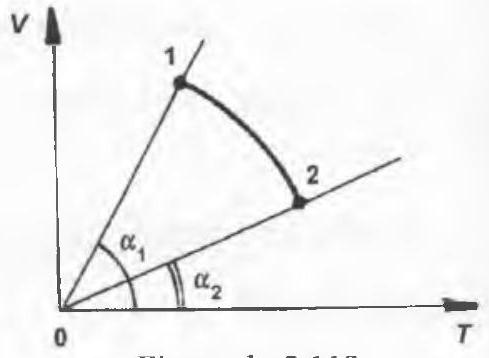
\includegraphics[max width=\textwidth, center]{2025_07_01_5b3ff9fa0d508c8e9f17g-293(1)}\\ FIgura problemei \end{center}\\

2.114. $p=\frac{1}{3} n m_{0}\left\langle v^{2}\right\rangle=\frac{1}{3} n\left(\frac{\mu}{N_{A}}\right) v_{T}^{2} \Rightarrow n=\frac{N_{A} \cdot 3 p}{\mu v_{T}^{2}}=10^{25} \mathrm{~m}^{-3}$;\\ Deci densitatea este: $\rho=n m_{0}=\frac{3 p}{v_{T}^{2}}=0,545 \mathrm{~kg} / \mathrm{m}^{3}$.\\

2.115. Conservarea numărului de moli se scrie:\\ $\nu_{1}+k \nu_{1}=(1+k) \nu_{1}=\nu^{\prime}$.\\ Scriem ecuațiile de stare:\\ $p_{1} V=\nu_{1} R T \Rightarrow \nu_{1}=\frac{p_{1} V}{R T}=p_{1} \frac{n V_{2}}{R T};$\\ $p^{\prime}\left(n V_{2}+V_{2}\right)=\nu^{\prime} R T \Rightarrow \nu^{\prime}=\frac{p^{\prime}(n+1) V_{2}}{R T}$;\\ Deci: $p_{1}(1+k) \frac{n V_{2}}{R T}=\frac{p^{\prime}(n+1) V_{2}}{R T} \Rightarrow p^{\prime}=\frac{p_{1}(1+k) n}{n+1}=155,6 \frac{\mathrm{kN}}{\mathrm{m}^{2}}$.\\

2.116. La echilibru cele două gaze capătă aceeaşi temperatură. Deoarece temperatura este determinată de energia cinetică medie de translație, rezultă egalitatea energiilor cinetice de translație la echilibru.\\

2.117. Căldura nu se poate transforma integral în lucru mecanic.\\

2.118. $\frac{\nu C_{V} T_{1}}{2}=\nu C_{V}\left(T_{2}-T_{1}\right)+\nu C_{p}\left(T_{3}-T_{2}\right) \quad (1)$.\\ Legea izocorei: $\frac{p_{2}}{p_{1}}=\frac{T_{2}}{T_{1}} \Rightarrow \frac{1}{k}=\frac{T_{2}}{T_{1}} \Rightarrow T_{2}=\frac{T_{1}}{k}$;\\ Legea izobarei: $\frac{V_{3}}{T_{3}}=\frac{V_{2}}{T_{2}} \Rightarrow T_{3}=T_{2} \frac{V_{3}}{V_{2}}=T_{2} k$;\\ Avem relațiile $T_{3}=k \frac{T_{1}}{k}=T_{1}$, $C_{p}=C_{V}+R$.\\ Rescriem relaţia (1):\\ $\frac{1}{2} C_{V} T_{1}=C_{V}\left(\frac{T_{1}}{k}-T_{1}\right)+\left(C_{V}+R\right)\left(T_{1}-\frac{T_{1}}{k}\right)$;\\ $\frac{C_{V} T_{1}}{2}=C_{V} T_{1}\left(\frac{1-k}{k}\right)+C_{V} T_{1}-C_{V} \frac{T_{1}}{k}+R T_{1}-R \frac{T_{1}}{k}$;\\ $\frac{C_{V}}{2}=C_{V}\left[\frac{1-k}{k}+1-\frac{1}{k}\right]+R\left(\frac{k-1}{k}\right)$;\\ Obținem:\\ $\frac{C_{V}}{2 R}=\frac{k-1}{k} \Rightarrow k C_{V}=2 R k-2 R \Rightarrow k\left(2 R-C_{V}\right)=2 R \Rightarrow k=\frac{2 R}{2 R-\frac{3}{2} R}=\frac{4 R}{R}=4$.\\ \begin{center} 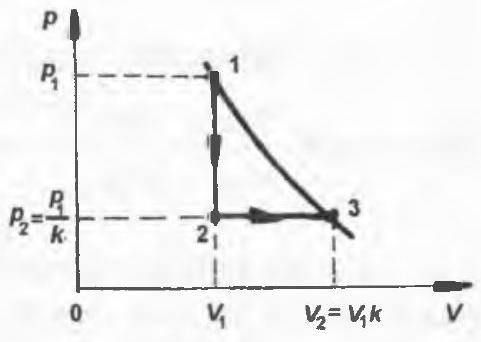
\includegraphics[max width=\textwidth]{2025_07_01_5b3ff9fa0d508c8e9f17g-293}\\ Figura problemei \end{center}\\

2.119. Ecuația Clapeyron ne permite să scriem $\frac{p V}{T}=\frac{p_{x} \cdot V(1+n)}{T-\Delta T}$.\\ Rezultă: $p_{x}=p \cdot \frac{1-\frac{\Delta T}{T}}{1+n}=1,5 \mathrm{~atm}$.\\

2.120. Randamentul va fi dat de:\\ $\eta=1+\frac{Q_{2}}{Q_{1}}=1+\frac{Q_{12}+Q_{23}}{Q_{34}+Q_{41}}=\frac{R}{2 R+C_{V}}=2 / 9$.\\

2.121. Plecând de la $\eta_{2}=\frac{P}{P_{C}}=\frac{P \cdot t}{L_{\text {util motor}}}$ şi $\eta_{1}=\frac{L_{\text {util motor}}}{Q_{1}}=\frac{L_{\text {util motor}}}{L_{\text {util motor}}+\left|Q_{\text {răcire}}\right|}$, obținem:\\ $Q_{\text {rācire}}=\frac{P t\left(1-\eta_{1}\right)}{\eta_{1} \eta_{2}}$.\\

2.122. Deoarece nu există tranziţii de fază, ecuația calorimetrică are forma:\\ $\sum_{k=1}^{k=4} m_{k} \cdot c \cdot\left(t-t_{k}\right)=0 \Rightarrow t=\frac{\sum_{k=1}^{k=4} m_{k} \cdot t_{k}}{\sum_{k=1}^{k=4} m_{k}}=32,3^{\circ} \mathrm{C}$.\\

2.123. Răspuns corect D).\\

2.124. Avem $\mu=m \cdot N_{A}=m R / k$.\\

2.125. Din primul principiu al termodinamicii, rezultă răspunsul corect D).\\

2.126. Gazul din piston suferă o transformare la volum constant, deci $\frac{p_{1}}{T_{1}}=\frac{p_{2}}{T_{2}}$, unde presiunea $p_{1}$ este presiunea inițială din piston: $p_{1}=p_{0}+m g / S$, cu $p_{0}$ presiunea atmosferică, $m$ masa pistonului, $g$ accelerația gravitațională, iar $p_{2}$ este presiunea finală din piston: $p_{2}=p_{0}+\left(m+m_{x}\right) g / S$, unde $m_{x}$ este masa care trebuie pusă deasupra pistonului pentru ca volumul acestuia să rămână constant. Înlocuind în prima relație se obține:\\ $\frac{p_{1}}{T_{1}}=\frac{p_{1}+\frac{m_{x} g}{S}}{T_{2}}$, de unde: $m_{x}=\frac{p_{1} S}{g}\left(\frac{T_{2}}{T_{1}}-1\right)=6,6 \mathrm{~kg}$.\\

2.127. Între căldurile specifice există relațiile: $c_{p}=c_{V}+\frac{R}{\mu}$ şi $\frac{c_{p}}{c_{V}}=\gamma$. Din aceste relaţii se obține:\\ $c_{V}=\frac{R}{\mu(\gamma-1)}=692,5 \mathrm{~J} / \mathrm{kg} \cdot \mathrm{K}$, $c_{p}=\frac{R \gamma}{\mu(\gamma-1)}=969,5 \mathrm{~J} / \mathrm{kg} \cdot \mathrm{K}$\\

2.128. Randamentul unei maşini termice este: $\eta=\frac{Q_{p}-Q_{c}}{Q_{p}}=1-\frac{Q_{c}}{Q_{p}}$.\\ Într-un ciclu Carnot: $\left|Q_{c}\right|=L_{\text {izot}}^{\prime}$ şi $\left|Q_{p}\right|=L_{\text {izot}}$, unde $L_{\text {izot}}^{\prime}$ este lucrul mecanic consumat de gaz la comprimarea izotermă. Înlocuind în expresia randamentului se obține: $\eta=1-\frac{L_{\mathrm{izot}}^{\prime}}{L_{\mathrm{izot}}} \Rightarrow L_{\mathrm{izot}}^{\prime}=60 \mathrm{~J}$.\\

2.129. Viteza pătratică medie la temperatura $t_{0}=0^{\circ} \mathrm{C}$ este $\sqrt{\overline{v_{0}^{2}}}=\sqrt{\frac{3 R T_{0}}{\mu}}$. Viteza pătratică medie la temperatura $t_{1}$ este $\sqrt{\overline{v_{1}^{2}}}=\sqrt{\frac{3 R T_{1}}{\mu}}$. Raportul celor două relații este $\frac{\sqrt{\overline{v_{1}^{2}}}}{\sqrt{\overline{v_{0}^{2}}}}=\sqrt{\frac{T_{1}}{T_{0}}}=2$, de unde: $T_{1}=4 T_{0}=1092 \mathrm{~K}$ sau $t_{1}=819^{\circ} \mathrm{C}$.\\

2.130. Scriem ecuațiile de stare:\\ $p V_{1}=\frac{m_{1}}{\mu} R T_{1} \Rightarrow m_{1}=\frac{\mu p V_{1}}{R T_{1}}$;\\ $p V_{2}=\frac{m_{2}}{\mu} R T_{2} \Rightarrow m_{2}=\frac{\mu p V_{2}}{R T_{2}}$.\\ Se observă că $m_{1}>m_{2}$, deoarece $T_{1}>T_{2}$, deci:\\ $\Delta m=m_{1}-m_{2}=\frac{\mu V}{R}\left(\frac{p_{1}}{T_{1}}-\frac{p_{2}}{T_{2}}\right)=5,39 \mathrm{~kg}$.\\

2.131. În urma procesului de încălzire, deoarece $T_{1}>T_{2}$ şi în acelaşi timp şi $p_{1}>p_{2}$ se poate presupune că în urma acestui proces gazul din primul compartiment îşi măreşte volumul cu $\Delta V_{1}$, iar cel din al doilea compartiment îşi micşorează volumul cu $\Delta V_{1}$. Pentru fiecare compartiment se pot scrie relațiile:\\ $\frac{p_{1} V_{1}}{T}=\frac{p^{\prime}\left(V_{1}+\Delta V_{1}\right)}{T_{1}}$; \quad $\frac{p_{2} V_{2}}{T}=\frac{p^{\prime}\left(V_{2}-\Delta V_{1}\right)}{T_{2}}$, unde $p^{\prime}$ este presiunea finală, aceeaşi în cele două compartimente.\\ Din relațiile precedente se obţine $\Delta V_{1}=V_{1} V_{2} \frac{p_{1} T_{1}-p_{2} T_{2}}{p_{1} V_{1} T_{1}+p_{2} V_{2} T_{2}}=10^{-3} \mathrm{~m}^{3}$.\\ Deci: $V_{1}^{\prime}=V_{1}+\Delta V_{1}=2 \cdot 10^{-3} \mathrm{~m}^{3}$, iar $V_{2}^{\prime}=V_{2}-\Delta V_{1}=10^{-3} \mathrm{~m}^{3}$.\\

2.132. Masa oxigenului din balon este $m=V \rho$, unde $\rho$ este densitatea gazului la temperatura $t=7^{\circ} \mathrm{C}$. Densitatea gazului la o temperatură oarecare $T$ în funcţie de densitatea gazului la temperatura $T_{0}$ este dată de relaţia: $\rho=\rho_{0} \frac{p}{p_{0}} \frac{T_{0}}{T}$.\\ Înlocuind se obține: $m=\rho V_{0} \frac{p}{p_{0}} \frac{T_{0}}{T}=0,139 \mathrm{~kg}$.\\ Căldura primită de gaz este: $Q=m c\left(t_{2}-t_{1}\right)=1280 \mathrm{~J}$.\\

2.133. Pentru un gaz are loc o transformare izotermă:\\ $p_{0} d_{1} S=p_{2} d_{2} S \Rightarrow$ $p_{2}=p_{0} \frac{d_{1}}{d_{2}}$;\\ Forța asupra pistonului este: $F=\left(p_{2}-p_{0}\right) S=p_{0}\left(\frac{d_{1}}{d_{2}}-1\right) S=30 \cdot 10^{3} \mathrm{~N}$.\\

2.134. Din ecuaţia de stare, $p V_{1}=\frac{m}{\mu} R T_{1} \Rightarrow V_{1}=\frac{m}{\mu} \cdot \frac{R T_{1}}{p}$.\\ Legea izobarei: $\frac{V_{1}}{T_{1}}=\frac{V_{2}}{T_{2}} \Rightarrow \frac{V_{2}}{V_{1}} T_{1}=\frac{V_{2} p \mu}{m R}$;\\ Obținem:\\ $Q=\nu C_{p} \Delta T=\frac{m}{\mu} \cdot \frac{7}{2} R \cdot\left(\frac{V_{2} p \mu}{m R}-T_{1}\right)=7927,8 \mathrm{~J}$;\\ $\Delta U=Q-L=Q-p \Delta V=5662,8 \mathrm{~J}$.\\

2.135. $Q_{p}=\nu\left[C_{p}\left(T_{2}-T_{1}\right)+C_{V}\left(T_{1}-T_{4}\right)\right]$;\\ Din ecuaţia de stare, $p V=\nu R T \Rightarrow T_{2}-T_{1}=\frac{4 V_{0} p_{0}}{\nu R}$;\\ Avem $T_{1}-T_{4}=\frac{V_{0} p_{0}}{\nu R} \Rightarrow Q_{p}=\frac{33}{2} V_{0} p_{0}$;\\ Deoarece $L=2 V_{0} p_{0}$, obţinem $\eta=\frac{L}{Q_{p}}=\frac{4}{33}=12,12 \%$.\\

2.136. $L=p \Delta V=\nu R\left(T_{B}-T_{A}\right) \Rightarrow T_{B}=T_{A}+\frac{L}{\nu R}=520 \mathrm{~K}$.\\

2.137. Scriem legea gazelor pentru cele două stări:\\ $p_{2} V=\nu R T_{2} \quad (1)$\\ $p_{1} V=\nu R T_{1} \quad (2)$\\ Din relația (1) scădem relația (2) şi obținem:\\ $\left(p_{2}-p_{1}\right) V=\nu R\left(T_{2}-T_{1}\right) \quad (3)$\\ Împărțim relația (3) la (1), rezultă $\frac{p_{2}-p_{1}}{p_{2}}=\frac{T_{2}-T_{1}}{T_{2}}$, de unde obținem:\\ $\frac{\Delta p}{p_{2}}=\frac{400-200}{400}=\frac{200}{400}=0,5=50 \%$.\\

2.138. Randamentul ciclului Carnot este:\\ $\eta=1-\frac{T_{2}}{T_{1}}=1-\frac{300}{400}=1-\frac{3}{4}=1-0,75=0,25$;\\ Dar, randamentul ciclului Carnot poate fi scris și sub forma:\\ $\eta=\frac{L}{Q_{1}}\ (1)$ sau $\eta=\frac{Q_{1}-Q_{2}}{Q_{1}}\ (2)$, unde $Q_{1}$ este căldura primită de la sursa caldă $\left(T_{1}\right)$, iar $Q_{2}$ este căldura cedată sursei reci $\left(T_{2}\right)$.\\ Din relația (1) găsim: $Q_{1}=\frac{L}{\eta}=\frac{80}{0,25} \mathrm{~kJ}=\frac{8000}{25} \mathrm{~kJ}=320 \mathrm{~kJ}$.\\ Din numitorii relațiilor (1) și (2) rezultă:\\ $Q_{2}=L-Q_{1}=(320-80) \mathrm{kJ}=240 \mathrm{~kJ}$.\\

2.139. Folosind legea gazului ideal scrisă sub forma $\frac{p V}{T}=$ const. şi datele din figura problemei, putem scrie:\\ În transformarea $1 \rightarrow 2$:\\ $\frac{p_{1} V_{1}}{T_{1}}=\frac{p_{2} V_{2}}{T_{2}}=\frac{3 p_{1} V_{1}}{T_{2}}$; \quad $T_{2}=3 T_{1} \quad (1)$\\ În transformarea $2 \rightarrow 3$:\\ $\frac{p_{2} V_{2}}{T_{2}}=\frac{p_{3} V_{3}}{T_{3}}$; \quad $\frac{3 p_{1} V_{1}}{T_{2}}=\frac{3 p_{1} 3 V_{1}}{T_{3}}$; \quad $T_{3}=3 T_{2}=9 T_{1} \quad (2)$\\ În transformarea $3 \rightarrow 4$:\\ $\frac{p_{3} V_{3}}{T_{3}}=\frac{p_{4} V_{4}}{T_{4}}$; \quad $\frac{3 p_{1} \cdot 3 V_{1}}{T_{3}}=\frac{3 V_{1} \cdot p_{1}}{T_{4}}$; \quad $T_{4}=\frac{T_{3}}{3}=\frac{9 T_{1}}{3}=3 T_{1} \quad (3)$\\ Din relația lui Robert Mayer rezultă: $C_{p}=C_{V}+R=\frac{5}{2} R+R=\frac{7}{2} R \quad (4)$\\ Randamentul unei maşini termice este dat de relația $\eta=\frac{L}{Q_{p}}\ (5)$, unde $L$ este lucrul mecanic efectuat de maşina termică, iar $Q_{p}$ ese cantitatea de căldură primită.\\ Lucrul mecanic efectuat este egal cu suprafața ciclului:\\ $L=\Delta p \Delta V=2 p_{1} \cdot 2 V_{1}=4 p_{1} V_{1}=4 \nu R T_{1}\ (6)$, $\nu$ fiind numărul de moli ai gazului folosit de maşina termică.\\ Conform datelor din relațiile (1), (2) şi (3), maşina termică primeşte căldură în transformările $1 \rightarrow 2$ şi $2 \rightarrow 3$. Deci:\\ $Q_{1 \rightarrow 2}=\nu C_{V}\left(T_{2}-T_{1}\right)=\nu C_{V}\left(3 T_{1}-T_{1}\right)=\nu C_{V} \cdot 2 T_{1}=2 \nu \frac{5}{2} R T_{1}=5 \nu R T_{1}$;\\ $Q_{2 \rightarrow 3}=\nu C_{p}\left(T_{3}-T_{2}\right)=\nu \frac{7}{2} R\left(9 T_{1}-3 T_{1}\right)=\nu \frac{7}{2} R 6 T_{1}=21 \nu R T_{1}$;\\ $Q_{p}=Q_{1 \rightarrow 2}+Q_{2 \rightarrow 3}=5 \nu R T_{1}+21 \nu R T_{1}=26 \nu R T_{1} \quad (7)$\\ Folosind (5), (6) şi (7), randamentul maşinii termice este:\\ $\eta=\frac{L}{Q_{p}}=\frac{4 \nu R T_{1}}{26 \nu R T_{1}}=\frac{2}{13}$.\\ \begin{center} 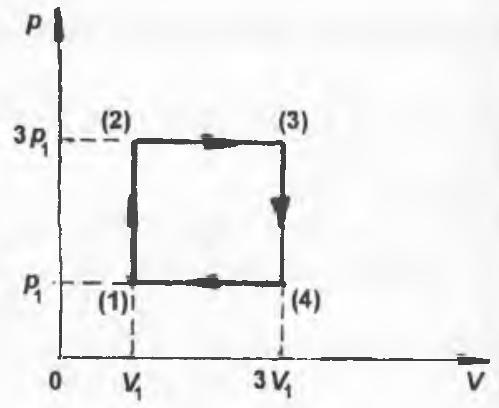
\includegraphics[max width=\textwidth]{2025_07_01_5b3ff9fa0d508c8e9f17g-297}\\ Figura problemei \end{center}\\

2.140. Când corpul pompei este pentru prima datǎ în contact cu vasul, presiunea devine aceeaşi în ambele volume.\\ Deci: $p_{0} V=p_{1}\left(V+V_{0}\right)$ şi $p_{1}=p_{0}\left(\frac{V}{V+V_{0}}\right)$ (1) este presiunea aerului din vas după prima cursă.\\ La a doua cursă:\\ $p_{1} V=p_{2}\left(V+V_{0}\right)$ şi $p_{2}=p_{1}\left(\frac{V}{V+V_{0}}\right)=p_{0}\left(\frac{V}{V+V_{0}}\right)^{2}$ (2), care este presiunea aerului din vas după a doua cursă.\\ Folosind legea inducției matematice, presiunea aerului din vas după "$n$" curse va fi:\\ $p_{n}=p_{0}\left(\frac{V}{V+V_{0}}\right)^{n}$.\\ Din ultima relație şi datele problemei obținem:\\ $\left(\frac{V+V_{0}}{V}\right)^{n}=\frac{p_{0}}{p_{n}}=\frac{p_{0}}{10^{-4} p_{0}}=10^{4}$ sau $\left(\frac{V+V_{0}}{V}\right)^{n}=10^{4}$.\\ Prin logaritmarea ultimei relații obținem $n \lg \left(\frac{V+V_{0}}{V}\right)=4$, de unde rezultă numǎrul de curse: $n=\frac{4}{\lg \left(\frac{V+V_{0}}{V}\right)}$.\\

2.141. Din teoria cinetico-moleculară a gazelor, presiunea gazului are formula: $p=\frac{1}{3} n m \overline{v^{2}}$ (1), unde $m$ este masa unei molecule, $\overline{v^{2}}$ este media lui $v^{2}$, iar $n=N / V$ este concentrația moleculelor. Transformarea este izocoră: $V=$ constant şi $n=N / V=$ constant.\\ Din relația (1) obținem pentru viteza termică a moleculelor expresia:\\ $v_{T}=\sqrt{\overline{v^{2}}}=\sqrt{\frac{3 p}{n m}}$ (2)\\ Aplicând relația (2) pentru cele două situaţii din enunţul problemei, obținem: $v_{T_{1}}=\sqrt{\frac{3 p_{1}}{n m}}$ (3) și $v_{T_{2}}=\sqrt{\frac{3 p_{2}}{n m}}$ (4)\\ Împǎrțind relația (3) la (4), obținem:\\ $\frac{v_{T_{1}}}{v_{T_{2}}}=\sqrt{\frac{p_{1}}{p_{2}}}=\sqrt{\frac{p_{1}}{4 p_{1}}}=\sqrt{\frac{1}{4}}=\frac{1}{2}$.\\

2.142. Conform legii de dilatare, putem scrie:\\ $l=l_{0}(1+\alpha \Delta t)$; $\Delta l=l_{0} \alpha \Delta t$;\\ $\gamma=3 \alpha \Rightarrow \alpha=\gamma / 3$ şi $\frac{\Delta l}{l_{0}}=\frac{\gamma \Delta t}{3}$ (1)\\ Din legea lui Hooke aflǎm forța: $\frac{F}{S}=E \frac{\Delta l}{l_{0}} \Rightarrow F=E \cdot S \cdot \frac{\Delta l}{l_{0}}$ (2)\\ Înlocuind (1) în (2), găsim:\\ $F=\frac{S E \gamma \Delta t}{3}=\frac{10^{-3} \cdot 2 \cdot 10^{11} \cdot 33 \cdot 10^{-6} \cdot 10^{2}}{3} \mathrm{~N}=22 \cdot 10^{10} \mathrm{~N}$.\\

2.143. La echilibru termic temperatura finală $\left(t_{f}\right)$ a apei este aceeaşi. Deci:\\ $m c\left(t_{f}-t_{1}\right)=3 m c\left(t_{2}-t_{f}\right)$; \quad $t_{f}(m c+3 m c)=3 m c t_{2}+m c t_{1}$;\\ $4 m c t_{f}=3 m c t_{2}+m c t_{1}$;\\ Rezultă: $t_{f}=\frac{3 t_{2}+t_{1}}{4}=\frac{3 \cdot 60+40}{4}=\frac{180+40}{4}=\frac{220}{4}=55^{\circ} \mathrm{C}$.\\

2.144. Cu notațiile din figura problemei, avem:\\ $\left.\begin{array}{l} p_{A} V_{A}=\nu R T_{A}\\ p_{0} V_{1}=\nu R T_{B}\\ p_{0} V_{2}=\nu R T_{f} \end{array}\right\} \Rightarrow \frac{p_{A} V_{A}}{T_{A}}=\frac{p_{0} V_{1}}{T_{B}}=\frac{p_{0} V_{2}}{T_{f}}$;\\ $\Delta U+L=0$ (convenție $\mathrm{d} L=+p \mathrm{~d} V$);\\ $\nu C_{V}\left(T_{f}-T_{A}\right)+\nu C_{V}\left(T_{f}-T_{B}\right)+p_{0}\left(V_{2}-V_{1}\right)=0$;\\ Dar $p_{0}\left(V_{2}-V_{1}\right)=\nu R\left(T_{f}-T_{B}\right)$, deci:\\ $\nu C_{V}\left(T_{f}-T_{A}\right)+\nu C_{V}\left(T_{f}-T_{B}\right)+\nu R\left(T_{f}-T_{B}\right)=0$;\\ $T_{f}=\frac{C_{V} T_{A}+C_{V} T_{B}+R T_{B}}{2 C_{V}+R}=\frac{C_{V} T_{A}+C_{p} T_{B}}{C_{V}+C_{p}}$;\\ Avem $C_{V}=\frac{3}{2} R$; \quad $C_{p}=C_{V}+R=\frac{5}{2} R$;\\ Obținem: $T=\frac{\frac{3}{2} R T_{A}+\frac{5}{2} R T_{B}}{\frac{3}{2} R+\frac{5}{2} R}=337,5 \mathrm{~K}$.\\ \begin{center} 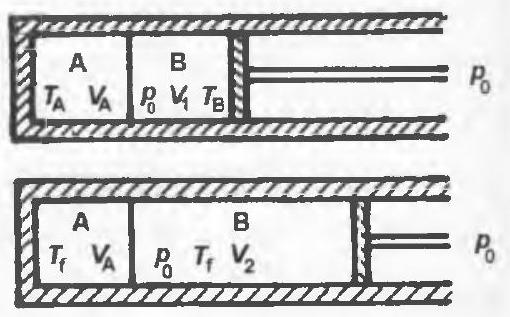
\includegraphics[max width=\textwidth]{2025_07_01_5b3ff9fa0d508c8e9f17g-299}\\ Figura problemei \end{center}\\

2.145. $v_{T_{1}}=\sqrt{\frac{3 R T_{1}}{\mu}} \Rightarrow T_{1}=\frac{\mu v_{T_{1}}^{2}}{3 R}$;\\ $v_{T_{2}}=\sqrt{\frac{3 R T_{2}}{\mu}} \Rightarrow T_{2}=\frac{\mu v_{T_{2}}^{2}}{3 R}$;\\ Obținem variația energiei interne:\\ $\Delta U=\nu C_{V}\left(T_{2}-T_{1}\right)=\frac{m}{\mu} \cdot \frac{5}{2} R \frac{\mu}{3 R}\left(v_{T_{2}}^{2}-v_{T_{1}}^{2}\right)=\frac{5}{6} m\left(v_{T_{2}}^{2}-v_{T_{1}}^{2}\right)=150 \mathrm{~J}$.\\

2.146. Avem $V_{2}=2 V_{1}$; \quad $p_{2}=2 p_{1}$;\\ Scriem ecuațiile de stare:\\ $\left.\begin{array}{l} p_{1} V_{1}=\nu R T_{1}\\ p_{2} V_{2}=\nu R T_{2}\\ p_{1} V_{2}=\nu R T_{3} \end{array}\right\} \Rightarrow T_{2}=4 T_{1}$, $T_{3}=2 T_{1}$;\\ De asemenea, $C_{V}=\frac{3}{2} R$, $C_{p}=\frac{5}{2} R$, $C_{12}=2 R$.\\ Lucrul mecanic este:\\ $L=\frac{1}{2}\left(p_{2}-p_{1}\right)\left(V_{2}-V_{1}\right)=\frac{1}{2} p_{1} V_{1}$;\\ În ceea ce privește căldurile,\\ $Q_{12}=\nu C_{12}\left(T_{2}-T_{1}\right)=\nu C_{12} \cdot 3 T_{1}=6 \nu R T_{1}=6 p_{1} V_{1}$;\\ $Q_{23}<0$; $Q_{31}<0$;\\ Obținem randamentul $\eta=\frac{L}{Q_{12}}=\frac{\frac{1}{2} p_{1} V_{1}}{6 p_{1} V_{1}}=\frac{1}{12}$.\\ Randamentul unui ciclu Carnot care ar funcționa în acest regim este:\\ $\eta_{c}=1-\frac{T_{1}}{T_{2}}=\frac{3}{4}$.\\

2.147. Vezi figura problemei.\\ Transformăm Celsius în Kelvin:\\ $t_{1}=227^{\circ} \mathrm{C} \Rightarrow T_{1}=500 \mathrm{~K}$;\\ $t_{2}=27^{\circ} \mathrm{C} \Rightarrow T_{2}=300 \mathrm{~K}$;\\ Randamentul ciclului Carnot: $\eta=1-\frac{T_{2}}{T_{1}}=1-\frac{300}{500}=0,4$;\\ Deoarece $\frac{V_{B}}{V_{A}}=\varepsilon=10$, avem:\\ $Q_{A B}=\nu R T_{1} \ln \frac{V_{B}}{V_{A}}=2,3 \nu R T_{1} \ln \varepsilon$;\\ Deci: $L=\eta Q_{A B}=3,818 \cdot 10^{6} \mathrm{~J}$.\\ \begin{center} 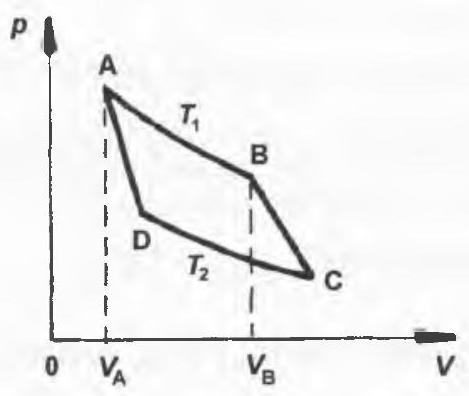
\includegraphics[max width=\textwidth]{2025_07_01_5b3ff9fa0d508c8e9f17g-300}\\ Figura problemei \end{center}\\

2.148. Se ştie că: $p=\frac{2}{3} n m \frac{\overline{v^{2}}}{2}=\frac{1}{3} n \frac{\mu}{N_{A}} \cdot v^{2}$ (1), unde $p$ este presiunea gazului, $n$ este concentrația moleculelor, $m$ este masa unei molecule, $v=\sqrt{\bar{v}^{2}}$ este viteza pătratică medie a moleculelor, $\mu$ este masa molară a gazului, iar $N_{A}$ este numărul lui Avogadro.\\ Din (1) găsim: $n=\frac{3 p N_{A}}{\mu v^{2}}=\frac{9}{14} \cdot 10^{23} \mathrm{~m}^{-3}$.\\

2.149. Din $p_{1} V_{1}=\nu R T_{1}$ obținem: $\nu_{1}=\frac{p_{1} V}{R T_{1}}=\frac{m_{1}}{\mu}$ (1);\\ Analog, $\nu_{2}=\frac{p_{2} V}{R T_{2}}=\frac{m_{1}-\Delta m}{\mu}$ (2).\\ Din (1) şi (2): $\Delta m=m_{1}-\mu \frac{p_{2} V}{R T_{2}}=\mu \frac{V}{R}\left(\frac{p_{1}}{T_{1}}-\frac{p_{2}}{T_{2}}\right)=20 \mathrm{~g}$.\\

2.150. Din primul principiu al termodinamicii:\\ $Q_{V}=\nu C_{V} \Delta T=\frac{m}{\mu} C_{V} \Delta T=10^{3} \mathrm{~J}$, unde $\mu=28 \frac{\mathrm{kg}}{\mathrm{kmol}}$ este masa kilomolară a azotului.\\

2.151. În transformarea izobară, $L=p\left(V_{2}-V_{1}\right)=\nu R\left(T_{2}-T_{1}\right)=v R \Delta T$ (1), însă $\nu=\frac{p_{1} V_{1}}{R T_{1}}$, astfel încât (1) se scrie:\\ $L=\frac{p_{1} V_{1}}{R T_{1}} R \Delta T \Rightarrow \Delta T=\frac{T_{1} L}{p_{1} V_{1}}=20 \mathrm{~K}$.\\

2.152. $\Delta U=\nu C_{V} \Delta T=\frac{C_{V}}{R} \nu R \Delta T=\frac{C_{V}}{R}\left(p_{2}-p_{1}\right) \cdot V=5 \cdot 10^{3} \mathrm{~J}$.\\

2.153. Folosim expresia randamentului $\eta=\frac{Q_{1}-\left|Q_{2}\right|}{Q_{1}}=\frac{L}{Q_{1}}$ (1), unde $L$ este lucrul mecanic efectuat pe un ciclu, iar $Q_{2}$ căldura cedată sursei reci.\\ Din (1), $L=\eta Q_{1}=1 \mathrm{~kJ}$.\\

2.154. Ecuația calorimetrică se scrie: $m_{a} c_{a} \Delta t_{1}=m c \Delta t_{2}$ (1), unde $m_{a}$, $m$ sunt masa apei, respectiv a metalului $c_{a}$, $c$ căldurile specifice pentru apă, respectiv metal.\\ Din (1): $c=\frac{m_{a} c_{a} \Delta t_{1}}{m \Delta t_{2}}=750 \mathrm{~J} / \mathrm{kg} \cdot \mathrm{K}$, unde $\Delta t_{1}=30^{\circ} \mathrm{C}$, $\Delta t_{2}=40^{\circ} \mathrm{C}$.\\

2.155. Echilibrul forţelor de presiune pentru tubul orizontal devine echilibrul (egalitatea) presiunilor, deoarece secțiunile de o parte şi cealaltă a pistonului sunt egale:\\ $p_{1}=p_{2}$, dar $p V=\frac{m}{\mu} R T \Rightarrow \frac{m_{1} R T_{1}}{V_{1} \mu_{1}}=\frac{m_{2} R T_{2}}{V_{2} \mu_{2}} \Rightarrow \frac{V_{1}}{V_{2}}=\frac{m_{1} T_{1} \mu_{2}}{m_{2} T_{2} \mu_{1}}$.\\

2.156. $p=$const. și $V=$ const. $\Rightarrow p V=$ const.\\ Din ecuaţia de stare $p V=\frac{m}{\mu} R T \Rightarrow \frac{m_{2}}{m_{1}}=\frac{T_{1}}{T_{2}} \Rightarrow \frac{m-\Delta m}{m}=\frac{T_{1}}{T_{2}} \Rightarrow m=\frac{T_{2} \Delta m}{T_{2}-T_{1}}$;\\ Cum $\rho=\rho_{0} \frac{T_{0}}{T_{1}} \Rightarrow \rho_{0}=\rho \frac{T_{1}}{T_{0}} \Rightarrow \rho_{0}=\frac{m}{V} \cdot \frac{T_{1}}{T_{0}}=\frac{T_{1} T_{2} \Delta m}{V T_{0}\left(T_{2}-T_{1}\right)}=\frac{\Delta m}{T_{2}-T_{1}} \cdot \frac{T_{1} T_{2}}{V T_{0}}$.\\

2.157. Gazul suferă o transformare izocoră:\\ $\frac{p_{2}}{p_{1}}=\frac{T_{2}}{T_{1}}$; $T_{2}=T_{1}+\Delta T \Rightarrow T_{1}+\Delta T=\frac{p_{2}}{p_{1}} T_{1} \Rightarrow T_{1}\left(\frac{p_{2}}{p_{1}}-1\right)=\Delta T$.\\ Deci: $T_{1}=\frac{\Delta T}{\frac{p_{2}}{p_{1}}-1} T_{1}=\frac{10}{10-1} \Rightarrow T_{1}=\frac{10}{9} \mathrm{~K} \cong 1,1 \mathrm{~K}$.\\

2.158. Recipientul de volum constant este izolat adiabatic de mediul exterior ($L=0$, $Q=0 \Rightarrow \Delta U=\Delta U_{1}+\Delta U_{2}=0$), rezultă ecuaţia calorimetrică:\\ $\Delta U_{1}+\Delta U_{2}=Q_{1 \nu}+Q_{2 \nu}=0 \Rightarrow \nu_{1} C_{V}\left(T-T_{1}\right)+\nu_{2} C_{V}\left(T-T_{2}\right)=0 \Rightarrow$\\ $\Rightarrow \nu_{1} C_{V} T+\nu_{2} C_{V} T=\nu_{1} C_{V} T+\nu_{2} C_{V} T_{2}=$ const., adică energia internă totală se conservǎ pentru stările inițială şi finală (de echilibru):\\ $T=\frac{\nu_{1} T_{1}+\nu_{2} T_{2}}{\nu_{1}+\nu_{2}}$.\\

2.159. Avem: $V=V_{0}(1+\gamma t)$, $m=\rho_{0} V_{0}$ şi $m^{\prime}=V \rho=\frac{\rho_{0}}{1+\gamma_{a} t} V_{0}(1+\gamma t) \Rightarrow$\\ $\Rightarrow \frac{m}{m^{\prime}}=\frac{1+\gamma_{a} t}{1+\gamma t} \Rightarrow \gamma_{a}=\frac{m(1+\gamma t)-m^{\prime}}{m^{\prime} t}=$ coeficientul de dilatare a apei.\\

2.160. În coordonate ($p, V$), lucrul mecanic schimbat de sistem este proporțional cu aria de sub curba care descrie evoluția gazului între starea inițialã $1$ și starea finală $2$. Conform convenției de semne, lucrul mecanic este pozitiv dacă este cedat de sistem exteriorului, caz în care sensul de parcurgere al curbei se face în sensul crescător al abscisei (axa volumelor). Aşadar răspunsul corect este E).\\

2.161. Energia internă este funcție de stare, prin urmare variația ei depinde doar de starea inițială şi de starea finală a sistemului şi nu depinde de modul în care sistemul evoluează între cele două stări. Raspunsul corect este F).\\

2.162. Ecuația termică de stare este $p V=\nu R T$, de unde, explicitând temperatura, obținem $T(V)=p V /(\nu R)$. În coordonate ($T, V$) şi pentru $p=$ const., relația precedentă reprezintă ecuația unei drepte de pantă $p /(\nu R)$ care trece prin originea sistemului de axe. Pentru o cantitate fixată de gaz ($\nu=$ const.), panta este maximă când presiunea este maximă şi reciproc, cu cât presiunea este mai mică, si panta este mai mică. Răspunsul corect este E).\\

2.163. Ecuația termică de stare este $p V=\nu R T$, de unde, explicitând presiunea, obținem $p(T)=\nu R T /(p V)$. În coordonate ($p, T$) şi pentru $V=$ const., relația precedentă reprezintă ecuația unei drepte de pantă $\nu R / V$ care trece prin originea sistemului de axe. Pentru o cantitate fixată de gaz ($\nu=$ const.), panta este invers proporținală cu volumul, deci este maximă atunci când volumul este minim. Răspunsul corect este A).\\

2.164. Energia internă este funcție de stare, prin urmare variația ei depinde doar de starea initială şi de starea finală a sistemului şi nu depinde de modul în care sistemul evoluează între cele două stări. Mai mult, în cazul gazelor ideale, şi pentru o cantitate fixată de gaz ($\nu=$ const.), energia internă este funcție doar de temperatură $U=U(T)$. Prin urmare, dacă toate stările inițiale sunt caracterizate de aceeaşi valoare $T_{1}$ a temperaturii şi toate stările finale au aceeaşi temperatură $T_{2}$, variația energiei interne este aceeaşi pentru toate cazurile reprezentate în figură.\\

2.165. Conform principiului întâi al termodinamicii, $\Delta U=Q-L$. Lucrul mecanic $L$ este pozitiv (efectuat de sistem împortriva mediului exterior) și are valoarea cea mai mare în transformarea a), iar valoarea cea mai mică în transformarea e), $L_{a}>L>L_{e}>0$, sau $Q_{a}-\Delta U_{a}>Q-\Delta U>Q_{e}-\Delta U_{e}>0$.\\ Pe de altă parte, energia internă fiind funcție de stare (variația ei depinzând doar de starea inițială şi de starea finală a sistemului şi nedepinzând de modul în care sistemul evoluează între cele două stări), variația ei este aceeaşi pentru toate transformările reprezentate $\Delta U=$ const.\\ Rezultă că $Q_{a}>Q>Q_{e}>0$, cantitatea de căldura fiind cea mai mică în procesul e) şi având valori pozitive (căldura este primită de sistem de la mediul exterior). Răspunsul corect este E).\\

2.166. Conform principiului întâi al termodinamicii, $\Delta U=Q-L$. Lucrul mecanic $L$ este negativ (primit de sistem de la mediul exterior) şi are valoarea cea mai mare în transformarea e), iar valoarea cea mai mică în transformarea a), $L_{a}<L<L_{0}<0$, sau $Q_{a}-\Delta U_{a}<Q-\Delta U<Q_{e}-\Delta U_{e}<0$.\\ Pe de altă parte, energia internă fiind funcţie de stare (variaţia ei depinzând doar de starea inițială şi de starea finală a sistemului şi nedepinzând de modul în care sistemul evoluează între cele două stări), variaţia ei este aceeaşi pentru toate transformările reprezentate $\Delta U=$ const.\\ Rezultă că $Q_{a}<Q<Q_{e}<0$, cantitatea de căldura fiind cea mai mică în procesul a) şi având valori negative (căldura este primită de sistem de la mediul exterior). Răspunsul corect este A).\\

2.167. În coordonate ($p, V$), lucrul mecanic schimbat de sistem este proporțional, în valoare absolută, cu aria de sub curba care descrie evoluția gazului între starea inițială $1$ şi starea finală $2$. Conform convenției de semne, lucrul mecanic este pozitiv dacă este cedat de sistem exteriorului, caz în care sensul de parcurgere al curbei se face în sensul crescător al abscisei (axa volumelor) și negativ în caz contrar. Aceasta decurge din faptul că integrala lucrului mecanic $\int_{V_{\text {inițial}}}^{V_{\text {final}}} p(V) \mathrm{d} V$ este pozitivă dacă $V_{\text {inițial}}<V_{\text {final}}$ şi negativă în caz contrar, ştiut fiind că $p(V)$ nu poate fi decât pozitivă. În cazurile ilustrate în figură avem $L_{a}<L_{b}<L_{c}<L_{d}<L_{e}<0$. Aşadar, răspunsul corect este a), deoarece, în valori negative, sistemul schimbă cu exteriorul lucrul mecanic cel mai mic în decursul procesului a).\\

2.168. Masa unei molecule de $\mathrm{CO}_{2}$ este $m_{0}=\frac{\mu_{\mathrm{CO}_{2}}}{N_{A}}$. Rezultă pentru numărul de molecule cuprinse într-un gram: $N=\frac{m}{m_{0}}=\frac{m N_{A}}{\mu_{\mathrm{CO}_{2}}}$, unde $\mu_{\mathrm{CO}_{2}}=44 \mathrm{~kg} / \mathrm{Kmol}$.\\ Deci $N=\frac{10^{-3} \cdot 6,023 \cdot 10^{26}}{44} \text { molecule }=1,36 \cdot 10^{22} \text { molecule }$.\\

2.169. Din ecuația termică de stare, rezultă:\\ $p_{0} V=\frac{m}{\mu} R T_{0} \Rightarrow \mu=\frac{\rho R T_{0}}{p_{0}}$, unde $p_{0}=1,013 \cdot 10^{5} \mathrm{~N} / \mathrm{m}^{2}$, $T_{0}=273,15 \mathrm{~K}$ şi $R=8310 \mathrm{~J} / \mathrm{kmol} \cdot \mathrm{K}$.\\ Astfel, $\mu=28 \mathrm{~kg} / \mathrm{kmol}$.\\ Masele kilomolare ale celor 6 gaze sunt:\\ $\mu_{\mathrm{He}}=4 \mathrm{~kg} / \mathrm{kmol}$, $\mu_{\mathrm{H}_{2}}=2 \mathrm{~kg} / \mathrm{kmol}$, $\mu_{\mathrm{C}_{2} \mathrm{H}_{2}}=26 \mathrm{~kg} / \mathrm{kmol}$;\\ $\mu_{\mathrm{N}_{2}}=28 \mathrm{~kg} / \mathrm{kmol}$, $\mu_{\mathrm{CO}_{2}}=44 \mathrm{~kg} / \mathrm{kmol}$, $\mu_{\mathrm{O}_{2}}=32 \mathrm{~kg} / \mathrm{kmol}$.\\ Răspuns corect: Azot ($\mathrm{N}_{2}$).\\

2.170. În procesul izobar avem: $\frac{L}{Q_{p}}=\frac{\nu R \Delta T}{\nu C_{p} \Delta T}=\frac{R}{C_{p}}=\frac{R}{C_{v}+R}=0,4=40 \%$.\\

2.171. Randamentul primului motor Carnot este:

$$
\eta=1-\frac{T_{2}}{T_{1}} \Rightarrow \frac{T_{2}}{T_{1}}=1-\eta .
$$

Cel de-al doilea motor Carnot are randamentul $\eta^{\prime}$ :

$$
\eta^{\prime}=1-\frac{T_{2}^{\prime}}{T_{1}^{\prime}} \text { unde } T_{2}^{\prime}=2 T_{2}, \text { iar } T_{1}^{\prime}-T_{2}^{\prime}=T_{1}-T_{2}\left(T_{1}^{\prime}=T_{2}^{\prime}+T_{1}-T_{2}\right)
$$

Rezultă:

$$
\eta^{\prime}=1-\frac{2 T_{2}}{2 T_{2}+T_{1}-T_{2}}=1-\frac{2 T_{2}}{T_{2}+T_{1}}=1-\frac{2}{1+\frac{T_{1}}{T_{2}}}=1-\frac{2}{1+\frac{1}{1-\eta}}=\frac{\eta}{2-\eta}
$$

Deci

$$
\eta^{\prime}=\frac{0,5}{2-0,5}=\frac{1}{3}=33,33 \% .
$$

2.172. Ţinând cont de expresiile vitezei pătratice medii şi a concentrației numărului de particule, avem $\frac{3 R T}{\mu} \cdot \frac{N}{V}=c t$. Din ecuația termică de stare obținem $\frac{R T}{\mu}=\frac{p V}{m}$, şi introducând în relația de mai sus, rezultă

$$
3 \frac{P V}{M} \cdot \frac{N}{V}=c t \Rightarrow p=c t .
$$

2.173. Pe transformarea $1 \rightarrow 2(p=a V)$ sistemul schimbă căldura:

$$
\begin{aligned}
Q_{12} & =\Delta U_{12}+L_{12}=v C_{v}\left(T_{2}-T_{1}\right)-\frac{p_{2}+p_{1}}{2}\left(V_{1}-V_{2}\right)= \\
& =v C_{v}\left(T_{2}-T_{1}\right)-\frac{a V_{1}+a V_{2}}{2}\left(V_{1}-V_{2}\right)= \\
& =v C_{v}\left(T_{2}-T_{1}\right)-\frac{a}{2}\left(V_{1}^{2}-V_{1}^{2}\right)=v C_{v}\left(T_{2}-T_{1}\right)-\frac{1}{2}\left(p_{1} V_{1}-p_{2} V_{2}\right)= \\
& =v C_{v}\left(T_{2}-T_{1}\right)-\frac{1}{2}\left(p R T_{1}-v R T_{2}\right)= \\
& =v\left(C_{v}+\frac{R}{2}\right)\left(T_{2}-T_{1}\right)<0
\end{aligned}
$$

Pe transformarea $3 \rightarrow 1$, căldura primită este: $Q_{31}=v R T_{1} \ln \frac{V_{1}}{V_{3}}>0$.\\
Astfel, randamentul acestui ciclu este:

$$
\eta=1-\frac{\left|Q_{12}\right|}{Q_{31}}=1-\frac{v\left(C_{v}+\frac{R}{2}\right)\left(T_{1}-T_{2}\right)}{v R T_{1} \ln \frac{V_{1}}{V_{3}}}=1-\frac{2\left(1-\frac{T_{2}}{T_{1}}\right)}{\ln \frac{V_{1}}{V_{3}}}
$$

(pentru gazul ideal $C_{v}=\frac{3}{2} R$ ).\\
Pentru transformarea adiabatică $2 \rightarrow 3$, avem:

$$
\begin{aligned}
& T_{2} V_{2}^{\gamma-1}=T_{1} V_{3}^{\gamma-1} \Rightarrow V_{3}=V_{2}\left(\frac{T_{2}}{T_{1}}\right)^{\frac{1}{\gamma-1}}=\frac{V_{1}}{2}\left(\frac{T_{2}}{T_{1}}\right)^{\frac{1}{\gamma-1}} \\
& \Rightarrow \ln \frac{V_{1}}{V_{3}}=\ln \left[2 \cdot\left(\frac{T_{1}}{T_{2}}\right)^{\frac{1}{\gamma-1}}\right]=\ln 2+\frac{1}{\gamma-1} \ln \left(\frac{T_{1}}{T_{2}}\right)
\end{aligned}
$$

Cu acestea, randamentul ciclului devine: $\eta=1-\frac{2\left(1-\frac{T_{2}}{T_{1}}\right)}{\ln 2+\frac{1}{\gamma-1} \ln \left(\frac{T_{1}}{T_{2}}\right)}$.\\
Temperaturile extreme atinse pe acest ciclu sunt $T_{\max }=T_{1}$ şi $T_{\min }=T_{2}$.\\
Astfel, $\eta_{c}=1-\frac{T_{2}}{T_{1}} \Rightarrow \frac{T_{2}}{T_{1}}=1-\eta_{c}$. Randamentul ciclului devine:

$$
\eta=1-\frac{2 \eta_{c}}{\ln 2-\frac{3}{2} \ln \left(1-\eta_{c}\right)}
$$

2.174. $Q=v C_{V} \Delta T+L_{12}+L_{23}+L_{34}$

$$
\begin{aligned}
& C_{V}=\frac{3}{2} R \quad ; \quad v=1 \mathrm{~mol} \\
L_{12}= & p_{1}\left(V_{2}-V_{1}\right)=p_{1} V_{2}-p_{1} V_{1}=p_{2} V_{2}-p_{1} V_{1}=; \quad L_{23}=0 \text { (izocor) } \\
= & v R\left(T_{2}-T_{1}\right)=v R \Delta T \\
L_{34}= & p_{3}\left(V_{4}-V_{3}\right)=p_{4} V_{4}-p_{3} V_{3}=v R \Delta T \\
& Q=v C_{V} \Delta T+v R \Delta T+v R \Delta T=\frac{7}{2} v R \Delta T=\frac{7}{2} \cdot 10^{-3} \cdot 8310 \cdot 100=\frac{7 R}{20} .
\end{aligned}
$$

2.175. $p V=\frac{m}{\mu} R T T=k p^{2} \quad k=$ constanta de proportionalitate


\begin{equation*}
p V=\frac{m}{\mu} R k p^{2} \Rightarrow p=\frac{\mu}{m R k} \cdot V \tag{1}
\end{equation*}


Ecuația (1) este o dreaptă ce trece prin originea sistemului de coordonate ( $p, V$ ), (Fig. prob. 2.175).

Lucrul mecanic $L$ este egal cu aria trapezului format. Adică:

$$
\begin{aligned}
L & =\frac{p_{1}+p_{2}}{2}\left(V_{2}-V_{1}\right)=\frac{p_{1}+p_{2}}{2}\left(\frac{p_{2} m R k}{\mu}-\frac{p_{1} m R k}{\mu}\right)= \\
& =\frac{p_{1}+p_{2}}{2} \cdot \frac{m R k}{\mu}\left(p_{2}-p_{1}\right)=k\left(p_{2}^{2}-p_{1}^{2}\right) \cdot \frac{m R}{2 \mu}=\frac{m R}{\mu} \cdot \frac{k p_{2}^{2}-k p_{1}^{2}}{2}= \\
& =\frac{m R}{\mu} \cdot \frac{T_{2}-T_{1}}{2}=831 \mathrm{~J} \\
& \quad \quad Q=\Delta U+L=\frac{3}{2} \cdot \frac{m}{\mu} R\left(T_{2}-T_{1}\right)+L=3,324 \mathrm{~kJ} .
\end{aligned}
$$

\begin{center}
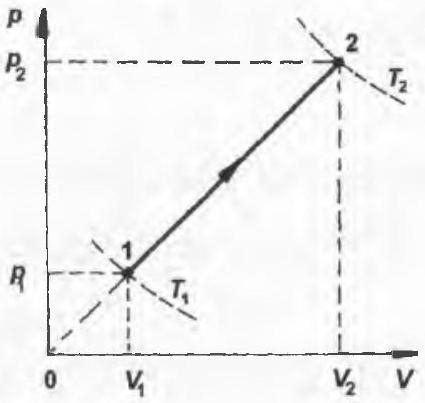
\includegraphics[max width=\textwidth]{2025_07_01_5b3ff9fa0d508c8e9f17g-307(1)}
\end{center}

Fig. prob. 2.175\\
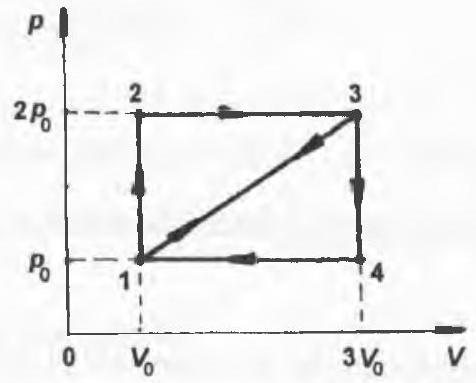
\includegraphics[max width=\textwidth, center]{2025_07_01_5b3ff9fa0d508c8e9f17g-307}

Fig. prob. 2.176\\
2.176. $T_{1}=T_{0} \quad T_{2}=2 T_{0} \quad T_{3}=6 T_{0} \quad T_{4}=3 T_{0} \quad C_{V}=\frac{3}{2} R \quad v=1 \mathrm{~mol}$

Notăm $\eta_{1}$ randamentul ciclului $1-2-3-1$ și cu $\eta_{2}$ randamentul ciclului 1-3-4-1.


\begin{gather*}
Q_{p_{1}}=C_{V} T_{0}+C_{p} \cdot 4 T_{0}=\frac{3}{2} R T_{0}+\frac{5}{2} \cdot 4 T_{0} R=\frac{3}{2} R T_{0}+\frac{20}{2} R T_{0}=\frac{23}{2} R T_{0} \\
L_{1}=\frac{p_{0}}{2} \cdot 2 V_{0}=p_{0} V_{0}=R T_{0} \\
\eta_{1}=\frac{L}{Q_{\text {primit } 123}}=\frac{2}{23} \tag{1}
\end{gather*}


Pentru ciclul 1-3-4-1 avem:

$$
\begin{aligned}
Q_{\text {primit }} & =Q_{1-3}=\Delta U_{1-3}+L_{13}=C_{V}\left(T_{3}-T_{0}\right)+\frac{p_{0}+2 p_{0}}{2} \cdot 2 V_{0}= \\
& =5 \cdot \frac{3}{2} R T_{0}+3 p_{0} V_{0}=\frac{15}{2} R T_{0}+3 R T_{0}=\frac{21}{2} R T_{0}
\end{aligned}
$$

Lucrul mecanic în acest ciclu este:


\begin{align*}
& L_{2}=R T_{0} \\
& \quad \eta_{2}=\frac{R T_{0}}{\frac{21}{2} R T_{0}}=\frac{2}{21} \tag{2}
\end{align*}


Din (1) şi (2) avem:

$$
\frac{\eta_{1}}{\eta_{2}}=\frac{21}{23}
$$

2.177. În starea inițială $\mathrm{O}_{2}$ satisface ecuația:


\begin{equation*}
p V_{1}=v_{1} R T_{1} \tag{1}
\end{equation*}


În starea inițială $\mathrm{N}_{2}$ satisface ecuația:


\begin{equation*}
p V_{2}=v_{2} R T_{2} \tag{2}
\end{equation*}


Pentru starea finală a amestecului avem:


\begin{equation*}
p\left(V_{1}+V_{2}\right)=\left(v_{1}+v_{2}\right) R T \tag{3}
\end{equation*}


Adunăm ecuația (1) şi (2) şi obținem:


\begin{equation*}
p\left(V_{1}+V_{2}\right)=v_{1} R T_{1}+v_{2} R T_{2} \tag{4}
\end{equation*}


Din ecuația (3) şi (4) rezultă:


\begin{equation*}
v_{1} T_{1}+v_{2} T_{2}=\left(v_{1}+v_{2}\right) T \tag{5}
\end{equation*}


sau

$$
T=\frac{v_{1} T_{1}+v_{2} T_{2}}{v_{1}+v_{2}}
$$

2.178. Randamentul ciclului Carnot este:

$$
\eta_{c}=\frac{T_{\mathrm{I}}-T_{2}}{T_{1}}=\frac{Q_{p}-\left|Q_{c}\right|}{Q_{p}}=1-\frac{\left|Q_{c}\right|}{Q_{p}}
$$

Din ecuațiile de mai sus şi din datele problemei avem:

$$
\begin{aligned}
Q_{c} & =\frac{70}{100} Q_{p}, \text { de unde } \\
\eta_{c} & =1-\frac{\frac{70}{100} Q_{p}}{Q_{p}}=\frac{3}{10} \text { si } \frac{T_{1}-T_{2}}{T_{1}}=\frac{3}{10} \Rightarrow \frac{400-T_{2}}{400}=\frac{3}{10} .
\end{aligned}
$$

Deci: $\quad T_{2}=280 \mathrm{~K}$.\\
2.179. Căldura la presiune constantă este dată de relația:

$$
\begin{aligned}
& Q_{p}=v C_{p} \Delta T \\
& p \Delta V=v R \Delta T \\
& Q_{p}=C_{p} \frac{p \Delta V}{R}
\end{aligned}
$$

Din sistemul:

$$
\left\{\begin{array}{l}
\frac{C_{p}}{C_{v}}=\gamma \\
C_{p}-C_{v}=R
\end{array}\right.
$$

se obține:

$$
C_{p}=\frac{\gamma R}{\gamma-1}
$$

Înlocuind în relația cantității de căldură se obține:

$$
Q_{p}=\frac{\gamma}{\gamma-1} p \Delta V=\frac{\gamma}{\gamma-1} p\left(V_{2}-V_{1}\right)=\frac{\gamma}{\gamma-1} p V_{1}\left(\frac{V_{2}}{V_{1}}-1\right)
$$

Rezultă: $\quad Q_{p}=4200 \mathrm{~J}$\\
2.180. Conform primului principiu al termodinamicii:

$$
\Delta U=U_{2}-U_{1}=Q-L
$$

Dar $\Delta U=0$, deoarece $U_{1}=U_{2}$, şi deci:

$$
Q=L
$$

Dar lucrul mecanic efectuat de sistem este:

$$
L=p \Delta V
$$

şi deci: $\quad \Delta V=\frac{L}{p}=\frac{Q}{p}=2,625 \mathrm{~m}^{3}$.\\
2.181. Din sistemul: $\left\{\begin{array}{l}\frac{c_{p}}{c_{V}}=\gamma \\ c_{p}-c_{V}=\frac{R}{\mu} \quad ; \text { unde } \mu \text { este masa moleculară a } \\ \rho_{0}=\frac{m}{V}=\frac{\mu p_{0}}{R T_{0}}\end{array}\right.$ gazului, se obține:

$$
c_{V}=\frac{R}{\mu(\gamma-1)}=\frac{p_{0}}{\rho_{0} T_{0}(\gamma-1)}
$$

$\operatorname{deci} c_{V}=717,4 \mathrm{~J} / \mathrm{kg} \mathrm{K}$.\\
Iar

$$
c_{p}=\gamma c_{V}=1004,36 \mathrm{~J} / \mathrm{kg} \mathrm{~K}
$$

2.182. Fie $T_{1}$ temperatura inițială a gazului pentru care viteza pătratică medie este $v_{1}$ şi $T_{2}$ temperatura gazului pentru care viteza pătratică medie este $v_{2}$. Dar viteza pătratică medie este de forma:

$$
v_{T}=\sqrt{\frac{3 R T}{\mu}} \text {; şi deci: } \quad \frac{v_{T_{2}}}{v_{T_{1}}}=\sqrt{\frac{T_{2}}{T_{1}}}=2 \Rightarrow \frac{T_{2}}{T_{1}}=4 .
$$

În starea inițială:

$$
p_{1} V=v R T_{1} ; \text { unde } v=\frac{m}{\mu} \text { este numărul de moli de gaz. }
$$

Căldura ce trebuie furnizată gazului într-o transformare izocoră este:

$$
Q=v C_{v} \Delta T=v C_{v}\left(T_{2}-T_{1}\right)=v C_{v} T_{1}\left(\frac{T_{2}}{T_{1}}-1\right)=\frac{m}{\mu} \frac{5}{2} R T_{1}\left(\frac{T_{2}}{T_{1}}-1\right)
$$

Înlocuind se obține

$$
Q=5842,9 \mathrm{~kJ}
$$

\begin{enumerate}
  \setcounter{enumi}{1}
  \item 
  \begin{enumerate}
    \setcounter{enumii}{182}
    \item Din ecuația Claperyon-Mendeleev:
  \end{enumerate}
\end{enumerate}

$$
p V_{1}=\frac{m}{\mu} R T_{1} \Rightarrow V_{1}=\frac{m}{\mu p} R T_{1}=8,31 \cdot 10^{-3} \mathrm{~m}^{3}
$$

iar:

$$
\rho_{1}=\frac{m}{V_{1}} \approx 2,40 \mathrm{~kg} / \mathrm{m}^{3}
$$

$$
p=\text { const. }
$$

$$
\frac{V_{1}}{T_{1}}=\frac{V_{2}}{T_{2}} \Rightarrow V_{2}=T_{2} \frac{V_{1}}{T_{1}}
$$

şi

$$
\rho_{2}=\frac{m}{V_{2}}=\frac{m T_{1}}{V_{1} T_{2}} \approx 1,26 \mathrm{~kg} / \mathrm{m}^{3}
$$

2.184. Pentru starea inițială legea generală a gazelor este de forma:

$$
p V_{1}=\frac{m_{1}}{\mu} R T_{1} \Rightarrow m_{1}=\frac{\mu p V_{1}}{R T_{1}}
$$

Pentru starea finală legea generală a gazelor este de forma:

$$
p V_{1}=\frac{m_{2}}{\mu} R T_{1} \Rightarrow m_{2}=\frac{\mu p V_{2}}{R T_{2}}
$$

Deoarece $m_{1}>m_{2}$ rezultă:

$$
\Delta m=m_{1}-m_{2}=\frac{\mu V}{R}\left(\frac{p_{1}}{T_{1}}-\frac{p_{2}}{T_{2}}\right)=5,39 \mathrm{~kg}
$$

2.185. Pentru fiecare compartiment se pot scrie relațiile:

$$
\begin{aligned}
& \frac{p_{1} V_{1}}{T}=\frac{p^{\prime}\left(V_{1}+\Delta V_{1}\right)}{n T} \\
& p_{2} V_{2}=p^{\prime}\left(V_{2}-\Delta V_{1}\right)
\end{aligned}
$$

unde $\Delta V_{1}$ reprezintă creşterea de volum a gazului din primul compartiment în urma încălzirii, iar $p^{\prime}$ este presiunea finală aceeaşi în cele două compartimente.

Din relațiile precedente se obține:

$$
\Delta V_{1}=V_{1} V_{2} \frac{n p_{1}-p_{2}}{n p_{1} V_{1}+p_{2} V_{2}}=0,6 \cdot 10^{-3} \mathrm{~m}^{3} .
$$

2.186. Randamentul unei maşini termice ideale este:

$$
\eta=\frac{T_{1}-T_{2}}{T_{1}}=0,25 .
$$

Dar, randamentul unei maşini termice de orice natură este de forma:

$$
\eta=\frac{L}{Q_{1}}=\frac{Q_{1}-Q_{2}}{Q_{1}}
$$

de unde:\\
iar:

$$
\begin{aligned}
& Q_{1}=\frac{L}{\eta}=21,6 \mathrm{M} \mathrm{~J} \\
& Q_{2}=(1-\eta) Q_{1}=16,2 \mathrm{MJ} .
\end{aligned}
$$

2.187. $m=\frac{p V \mu}{R T}=0,64 \mathrm{~kg}$.\\
2.188. $\Delta m=m_{2}-m_{1}=\frac{p_{2} V \mu}{R T_{2}}-\frac{p_{1} V \mu}{R T_{1}}=\frac{V \mu}{R}\left(\frac{p_{2}}{T_{2}}-\frac{p_{1}}{T_{1}}\right)=6 \mathrm{~kg}$.\\
2.189. $\quad c_{p}=c_{v}+\frac{R}{\mu} ; \quad \mu=\frac{R}{c_{p}-c_{v}} \cong 28 \mathrm{~kg} / \mathrm{kmol}$.\\
2.190.

$$
\begin{aligned}
& L=\frac{m}{\mu} R \Delta T \\
& \left.\begin{array}{l}
\frac{p_{1} V_{1}}{T_{1}}=\frac{m}{\mu} R
\end{array}\right\} L=\frac{p_{1} V_{1}}{T_{1}} \Delta T \\
& \quad L=\frac{2 \cdot 10^{5} \cdot 3}{300} 60=120 \mathrm{~kJ}
\end{aligned}
$$

2.191. $\Delta U=v C_{v} \Delta T=v\left(C_{p}-R\right) \Delta T=(450 R) \mathrm{J}$.\\
2.192.

$$
Q_{p}=v C_{p} \Delta T=\frac{m}{\mu} C_{p} \Delta T \Rightarrow Q_{p}=(7 R) \mathrm{J}
$$

2.193.

$$
\left.\begin{array}{rl}
\eta= & \frac{\mathrm{Q}_{1}+Q_{2}}{Q_{1}} \\
\eta= & \frac{T_{1}-T_{2}}{T_{1}}
\end{array}\right\} \Rightarrow\left|Q_{2}\right|=Q_{1}\left(1-\frac{T_{1}-T_{2}}{T_{1}}\right)
$$

2.194. $C=m c ; m=\frac{C}{c}=1,75 \mathrm{~kg}$.\\
2.195. $p_{1} V_{1}=v R T_{1}$

$$
p_{1}=\frac{v R T_{1}}{V_{1}}=1,99 \cdot 10^{5} \mathrm{~N} / \mathrm{m}^{2}
$$

transformare izobară $p_{1}=p_{2} \cdot \frac{V_{1}}{T_{1}}=\frac{V_{2}}{T_{2}} \Rightarrow V_{2}=V_{1} \cdot \frac{T_{2}}{T_{1}}=1,5 V_{1}$

$$
L=p_{1}\left(V_{2}-V_{1}\right)=0,5 V_{1}=497,3 \mathrm{~J}
$$

2.196.

$$
\begin{aligned}
& Q=\Delta U \xrightarrow{\text { princ } I} L=0 \Rightarrow \text { proces izocor } \\
& Q=v C_{v} \Delta T \quad v=\frac{m}{\mu}=\frac{44,8}{28}=1,6 \mathrm{kmoli} \\
& \Delta T=\frac{Q}{v C_{v}}=\frac{3,324 \cdot 10^{6} \cdot 2}{1,6 \cdot 5 \cdot 8310}=100 \mathrm{~K}
\end{aligned}
$$

2.197. $P V=v R T \Rightarrow T=\frac{P V}{v R}=\frac{P V \mu}{m R}$

$$
V_{T}=\sqrt{\frac{3 R T}{\mu}}=\sqrt{\frac{3 R}{\mu} \cdot \frac{P V \mu}{m R}}=\sqrt{\frac{3 P V}{m}}=600 \mathrm{~m} / \mathrm{s}
$$

2.198. $p V=\frac{m}{\mu} R T \Rightarrow \rho=\frac{m}{V}=\frac{p \mu}{R T}$

$$
\begin{gathered}
v_{T}=\sqrt{\frac{3 R T}{\mu}} \Rightarrow v_{T}^{2}=\frac{3 R}{\mu} \Rightarrow \mu=\frac{3 R T}{v_{T}^{2}} \\
\Rightarrow \rho=\frac{p \mu}{R T}=\frac{p}{R T} \cdot \frac{3 R T}{v_{T}^{2}}=\frac{3 p}{v_{T}^{2}} ; \quad \rho=1 \mathrm{~kg} / \mathrm{m}^{3} .
\end{gathered}
$$

2.199.

$$
\begin{gathered}
\begin{array}{c}
p=p_{0}+\rho g x \\
x=l-\frac{2}{3} h
\end{array} \\
S=\frac{\pi d^{2}}{4}=12,56 \cdot 10^{-6} \mathrm{~m}^{2} \\
F=p \cdot S=\left[p_{0}+\rho g\left(l-\frac{2}{3} h\right)\right] S=1,28 \mathrm{~N} .
\end{gathered}
$$

\begin{center}
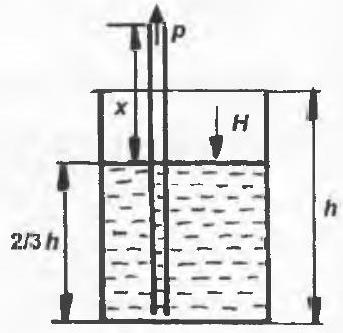
\includegraphics[max width=\textwidth]{2025_07_01_5b3ff9fa0d508c8e9f17g-313}
\end{center}

Fig. prob. 2.199\\

2.200. $p_{1} V_{1}=\nu_{1} R T_{1} ; \nu_{1}=\frac{p_{1} V_{1}}{R T_{1}}$\\ $p_{2}\left(V_{1}+V_{2}\right)=\nu_{1} R T_{2} \Rightarrow p_{2}=\frac{\nu_{1} R T_{2}}{V_{1}+V_{2}}=\frac{R T_{2}}{V_{1}+V_{2}} \cdot \frac{p_{1} V_{1}}{R T_{1}}$\\ $p_{2} V_{2}=\nu_{x} R T_{2}$\\ $p_{x}=\frac{p_{2} V_{2}}{R T_{2}}=\frac{p_{1} V_{1}}{T_{1}} \cdot \frac{T_{2}}{V_{1}+V_{2}} \cdot \frac{V_{2}}{R T_{2}}=\frac{p_{1}}{R T_{1}} \frac{V_{1} V_{2}}{V_{1}+V_{2}}$\\ $f=\frac{\nu_{x}}{\nu_{1}} \cdot 100=\frac{p_{1}}{R T_{1}} \cdot \frac{V_{1} V_{2}}{V_{1}+V_{2}} \cdot \frac{R T_{1}}{p_{1} V_{1}} \cdot 100=\frac{V_{2}}{V_{1}+V_{2}} \cdot 100=20 \%$\\

2.201. Pentru starea (1) avem:\\ $p_{1} V_{1}=\nu_{1} R T_{1}$\\ $p_{1}=\frac{\nu R T_{1}}{V_{1}}=1,6629 \cdot 10^{5} \mathrm{~N} / \mathrm{m}^{2}$\\ Din figură se observă că transformarea 1-2 este izobară deoarece $V=\frac{\nu R}{p} T=m T$, unde $m=\frac{\nu R}{p}$ este panta dreptei 1-2. Cum aceasta este constantă, rezultă $p=$ const. $\Rightarrow p_{2}=p_{1}=1,662 \cdot 10^{5} \mathrm{~N} / \mathrm{m}^{2}$.\\

2.202. Masa de apă încălzită este:\\ $m=\rho V=10 \mathrm{~kg}$\\ $Q=m c_{\text {apă }} \Delta t=2508 \cdot 10^{3} \mathrm{~J}$\\ $Q=P t \Rightarrow P=\frac{Q}{t}=2,09 \mathrm{~kW}$\\ $P=\frac{U^{2}}{R} \Rightarrow R=\frac{U^{2}}{P}=\frac{220 \cdot 220}{2,09 \cdot 10^{3}} \cong 23,15 \Omega$\\

2.203. Randamentul ciclului Carnot este:\\ $\eta_{C}=1-\frac{T_{2}}{T_{1}}=0,5$\\ $\eta_{\text {motor }}=0,6 \eta_{C}=0,3$\\ Forța de tracțiune (Fig. prob. 2.203):\\ $F=G \sin \alpha+\mu G \cos \alpha$\\ $F=m g(\sin \alpha+\mu \cos \alpha)=2873,85 \mathrm{~N}$\\ $\eta_{\text{motor}}=\frac{L_{\text{ef}}}{Q_{C}}$\\ $L_{\text{ef}}=$ lucrul mecanic efectuat de motor $=F d$\\ $Q_{C}=$ căldura consumată prin arderea combustibilului\\ $Q_{C}=m q$\\ $\eta_{\text{motor}}=\frac{F d}{m q} \Rightarrow m=\frac{F d}{\eta_{\text{motor}} \cdot q} \cong 0,68 \mathrm{~kg}$\\ \begin{center} 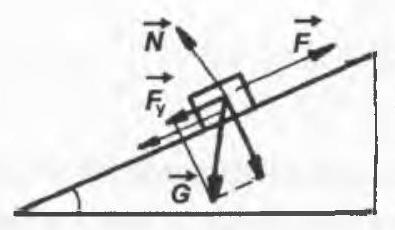
\includegraphics[max width=\textwidth, center]{2025_07_01_5b3ff9fa0d508c8e9f17g-314}\\ Fig. prob. 2.203 \end{center}\\

2.204. Folosind ecuațiile de stare pentru cele două stări ale sistemului, notate cu indicii 1 şi 2 , se obține: $p_{1} V_{1}=\nu R T_{1}$ (1), $p_{2} V_{2}=\nu R T_{2}$ (2). Din datele problemei se ştie că: $V_{2}=\frac{1}{3} V_{1}(3), T_{2}=4 T_{1}$ (4). Înlocuind (3), (4) în ecuațiile de stare (1), (2) şi fäcând raportul acestora, se obține:\\ $\frac{p_{1} V_{1}}{p_{2} \cdot \frac{1}{3} V_{1}}=\frac{\nu R T_{1}}{\nu R \cdot 4 T_{1}} \Rightarrow \frac{3 p_{1}}{p_{2}}=\frac{1}{4} \tag{5}$\\ Se obţine: $p_{2}=12 p_{1}$.\\

2.205. Lucrul mecanic efectuat în transformarea din starea (1) în starea (2) se calculează cu ajutorul formulei: $L=\int_{1}^{2} p \mathrm{~d} V$. În cazul problemei, volumul creşte de şapte ori, deci: $V_{2}=7 V_{1}$. Lucrul mecanic efectuat de gaz în transformarea izobară ( $p=$ const.) este: $L=\int_{1}^{2} p \mathrm{~d} V=p\left(V_{2}-V_{1}\right)=p\left(7 V_{1}-V_{1}\right)=6 p V_{1}$. Dacă scriem ecuația de stare pentru starea 1: $p V_{1}=\nu R T_{1}$, lucrul mecanic devine: $L=6 \nu R T_{1}$.\\ Căldura primită de sistem în transformarea izobară este: $Q=\nu C_{p} \Delta T=$ $=\nu C_{p}\left(T_{2}-T_{1}\right)$. Temperatura finală (în starea 2 ) se calculează cu ajutorul ecuaţiei de stare $p V_{2}=\nu R T_{2} \Rightarrow T_{2}=\frac{p V_{2}}{\nu R}=\frac{7 p V_{1}}{\nu R} ; T_{2}=7 T_{1}$. Inlocuind in expresia lui $Q$ se obține:\\ $Q=\nu C_{p}\left(7 T_{1}-T_{1}\right)=6 \nu C_{p} T_{1}=6 \nu \frac{5}{2} R T_{1}=15 \nu R T_{1}$\\ Raportul dintre lucrul mecanic $L$ şi căldura $Q$ este: $\frac{L}{Q}=\frac{2}{5}$.\\

2.206. Randamentul unei maşini termice ideale care funcționează după un ciclu Carnot este: $\eta=L / Q_{1}=\left(T_{1}-T_{2}\right) / T_{1}$. Temperatura sursei calde şi cea a sursei reci sunt cunoscute: $T_{1}=t_{1}+273 \mathrm{~K}=600 \mathrm{~K}, T_{2}=t_{2}+273 \mathrm{~K}=300 \mathrm{~K}$. Căldura primită de maşina termică, $Q_{1}$ fiind cunoscută, din prima relație se obține: $L=Q_{1} \frac{T_{1}-T_{2}}{T_{1}}$. Înlocuind valorile numerice, se obține rezultatul final:\\ $L=5 \cdot 10^{5} \mathrm{~J}$\\

2.207. La echilibru termic, căldura cedată de corpul cald din material plastic este egală cu cea acceptată de corpul mai rece (apa). $\left|Q_{\mathrm{pl}}\right|=Q_{\mathrm{ap}}$. Deci, $m_{\mathrm{pl}} c_{\mathrm{pl}}\left(t_{\mathrm{pl}}-t\right)=m_{\mathrm{ap}} c_{\mathrm{ap}}\left(t-t_{\mathrm{ap}}\right)$. Din datele problemei: $m_{\mathrm{ap}}=2 m_{\mathrm{pl}}$. Ca urmare, după simplificare, rezultă: $c_{\mathrm{pl}}\left(t_{\mathrm{pl}}-t\right)=2 c_{\mathrm{ap}}\left(t-t_{\mathrm{ap}}\right)$. Înlocuind valorile numerice, se obtine: $\frac{c_{\mathrm{ap}}}{c_{\mathrm{pl}}}=\frac{3}{2}$.\\

2.208. Deoarece sistemul ajunge din nou în starea inițială, el suferă o transformare ciclică. Lucrul mecanic şi căldura sunt mărimi care depind de stările intermediare prin care trece sistemul. Energia internă este o funcţie de stare care nu depinde decât de starea inițială şi de starea finală a transformării suferite de sistem. Ca urmare, variația energiei interne pentru o transformare ciclică este zero.\\

2.209. Să găsim parametrii gazului în fiecare din cele patru stări marcate:\\ A: $p_{A} ; V_{A}=0,2 \mathrm{~m}^{3} ; T_{A}$\\ B: $p_{B}=8 \cdot 10^{4} \mathrm{~N} / \mathrm{m}^{2} ; V_{B}=0,6 \mathrm{~m}^{3} ; T_{B}$\\ C: $p_{C}=5 \cdot 10^{4} \mathrm{~N} / \mathrm{m}^{2} ; V_{C}=0,6 \mathrm{~m}^{3} ; T_{C}$\\ D: $p_{D}=5 \cdot 10^{4} \mathrm{~N} / \mathrm{m}^{2} ; V_{D}=0,2 \mathrm{~m}^{3} ; T_{D}$\\ Transformarea $A B$ find izotermă $T_{A}=T_{B}$. În plus $p_{C}=p_{D} ; V_{B}=V_{C}$ şi $V_{D}=V_{A}$. Parametrii necunoscuți se determină din ecuațiile de stare:\\ $p_{B} V_{B}=\nu R T_{B} \Rightarrow T_{B}=\frac{p_{B} V_{B}}{\nu R} ; \quad \quad p_{C} V_{D}=\nu R T_{C} \Rightarrow T_{C}=\frac{p_{C} V_{C}}{\nu R}$\\ $p_{D} V_{D}=\nu R T_{D} \Rightarrow T_{D}=\frac{p_{D} V_{D}}{\nu R}$\\ Pentru starea $A$ avem: $p_{A} V_{A}=\nu R T_{B} \Rightarrow p_{A}=\frac{\nu R}{V_{A}} T_{B}=\frac{\nu R}{V_{A}} \cdot \frac{p_{B} V_{B}}{\nu R}=p_{B} \frac{V_{B}}{V_{A}} \Rightarrow$ $\Rightarrow p_{A}=\frac{V_{B}}{V_{A}}=24 \cdot 10^{4} \mathrm{~N} / \mathrm{m}^{2}$.\\ Afirmația 1) este corectă. Calculăm raportul $\frac{T_{C}}{T_{D}}$ folosind ecuațiile de stare.\\ $\frac{T_{C}}{T_{D}}=\frac{p_{C} V_{C}}{\nu R} \cdot \frac{\nu R}{p_{D} V_{D}} \Rightarrow \frac{T_{C}}{T_{D}}=\frac{V_{C}}{V_{D}}=3$. Afirmaţia 2) este falsă deoarece temperatura în $C$ este de trei ori mai mare (nu mai mică!) decât în $D$. Calculăm raportul $\frac{T_{B}}{T_{D}}$ folosind ecuatiile de stare.\\ $\frac{T_{B}}{T_{D}}=\frac{p_{B} V_{B}}{\nu R} \cdot \frac{\nu R}{p_{D} V_{D}} \Rightarrow \frac{T_{C}}{T_{D}}=\frac{p_{B} V_{B}}{p_{D} V_{D}}=4,8$\\ Afirmația 3) este corectă deoarece temperatura în $B$ creşte față de cea din $D$ de 4,8 ori. Transformarea $A B$ este izotermă şi nu adiabatică, ca urmare el schimbă căldură cu mediul exterior, ca urmare afirmația 4) este falsă.\\

2.210. Parametrii termodinamici în cele trei stări marcate sunt:\\ $A: p_{A}=2 \cdot 10^{4} \mathrm{~N} / \mathrm{m}^{2} ; V_{A}=0,3 \mathrm{~m}^{3} ; T_{A}$\\ $B: p_{B}=2 \cdot 10^{4} \mathrm{~N} / \mathrm{m}^{2} ; V_{B} ; T_{B}$\\ C: $p_{C}=5 \cdot 10^{4} \mathrm{~N} / \mathrm{m}^{2} ; V_{C}=0,6 \mathrm{~m}^{3} ; T_{C}$\\ Parametrii necunoscuți se determină din ecuațiile de stare:\\ $p_{A} V_{A}=\nu R T_{A} \Rightarrow T_{A}=\frac{p_{A} V_{A}}{\nu R} ; \quad \quad p_{B} V_{B}=\nu R T_{B} \Rightarrow T_{B}=\frac{p_{B} V_{B}}{\nu R}$\\ $\quad p_{C} V_{C}=\nu R T_{C} \Rightarrow T_{C}=\frac{p_{C} V_{C}}{\nu R}$\\ Transformarea $B C$ este adiabatică, ca urmare căldura schimbatǎ cu exteriorul este zero și nu lucrul mecanic, deci afirmația 1) este falsă. Temperaturile în $B$ și în $C$ diferă, deci şi afirmaţia 3) este falsă. Din relațiile de mai sus rezultă:\\ $\frac{T_{A}}{T_{C}}=\frac{p_{A} V_{A}}{\nu R} \cdot \frac{\nu R}{p_{C} V_{C}} \Rightarrow \frac{T_{A}}{T_{C}}=\frac{p_{A} V_{A}}{p_{C} V_{C}}=\frac{1}{5}$\\ Rezultă că afirmația 2) este adevărată. Pe ramura $C A$ sistemul cedează căldură deoarece $T_{C}<T_{A}$. Conform principiului fundamental al termodinamicii: $\Delta U=Q-L$. Pentru întreg ciclul $A B C A$ variația totalǎ a energiei interne este zero, deoarece aceasta este o mărime de stare. Ca urmare, lucrul mecanic efectuat este egal cu căldura totală schimbată cu exteriorul, adică diferența dintre căldura primită (ramura $A B$ ) şi cea cedată (ramura $C A$ ). $L=Q \Rightarrow L=Q_{A B}-Q_{C A}$. Afirmația 4) este falsă deoarece dacă ar transforma toată căldura primită în lucru mecanic, sistemul ar funcționa ca un perpetuum mobile de speta întâi, ceea ce este imposibil.\\ Din cele de mai sus rezultă că numai afirmaţia 2) este adevărată. Din numǎrul total de afirmaţii, numai una este adevărată.\\

2.211. Legea transformării izocore a gazului ideal este:\\ $p=p_{0}(1+\beta t)$ sau $\frac{p}{p_{0}}=1+\beta t$\\

2.212. Legea transformǎrii izobare a gazului ideal are expresia $V=V_{0}(1+\alpha t)$ sau $V-V_{0}=V_{0} \alpha t, V-V_{0}=\Delta V$ deci $\frac{\Delta V}{V_{0}}=\alpha t$.\\

2.213. Pentru a deduce unitatea de măsură pentru constanta lui Boltzmann, $k$, utilizăm relația de definiție $p=k n T$, unde $p=$ presiunea, $n=$ concentrația particulelor şi $T=$ temperatura. Deci:\\ $[k]=\frac{[p]}{[n \mathbf{I} T]}=\frac{\frac{\mathrm{N}}{\mathrm{~m}^{2}}}{\frac{1}{\mathrm{~m}^{3}} \cdot \mathrm{~K}}=\frac{\mathrm{J}}{\mathrm{~K}}$\\ Dar unitatea de măsură pentru capacitatea calorică: $[C]=\frac{\mathrm{J}}{\mathrm{K}}$.\\

2.214. Din ecuația termică de stare a gazului ideal: $p=m R T /(\mu V)$. O dreaptă care trece prin origine în coordonate ( $p, T$ ) are ecuația $p=a T$ unde $a=\operatorname{tg} \alpha$ este panta; $a \sim 1 / \mu$ dacă $m$ și $V$ sunt aceleaşi; $\mu_{\mathrm{CH}_{4}}>\mu_{\mathrm{H}_{2}}>\mu_{\mathrm{He}}$; dreapta 1 corespunde metanului.\\

2.215. Pentru sistemul format de cele două gaze: $Q_{\text {sist. }}=0$ (înveliş adiabatic) şi $L_{\text {sist. }}=0$ (volum total constant); din principiul întâi al termodinamicii: $Q=\Delta U+L$ rezultă $\Delta U=0$ deci $U_{\text {sist. }}=$ const.; $U_{i}=\nu_{1} C_{V} T_{1}+\nu_{2} C_{V} T_{2} ; U_{f}=\nu_{1} C_{V} T_{f}+\nu_{2} C_{V} T_{f}$; obținem:\\ $T_{f}=\frac{v_{1} T_{2}+v_{2} T_{2}}{v_{1}+v_{2}}=\frac{8 T}{9}$\\

2.216. $L=L_{12}+L_{21}$; pentru transformarea $1 \rightarrow 2$ calculăm lucrul mecanic prin aria de sub grafic, în coordonate $(p, V): L_{12}=\frac{\left(p_{1}+p_{2}\right)\left(V_{2}-V_{1}\right)}{2}$; din ecuația izotermei: $p_{2}=\frac{p_{1}}{2}$; rezultă: $L_{12}=\frac{3 p_{1} V_{1}}{4}$; pentru transformarea izotermă:\\ $L_{21} \nu R T_{1} \ln \frac{V_{1}}{V_{2}}=-p_{1} V_{1} \ln 2$\\ în final: $L=0,05 p_{1} V_{1}=\frac{p_{1} V_{1}}{20}$.\\

2.217. Din ecuaţia termică de stare: $m=\frac{p V \mu}{R T}$;\\ $\Delta m=m_{1}-m_{2}=\frac{p_{0} V \mu}{R}\left(\frac{1}{T_{1}}-\frac{1}{T_{2}}\right)$\\ dar: $\rho_{0}=\frac{p_{0} \mu}{R T_{0}}$; eliminând masa molară $\mu$ între ultimele două relații obținem:\\ $\rho_{0}=\frac{\Delta m T_{1} T_{2}}{V T_{0}\left(T_{2}-T_{1}\right)}=9,89 \mathrm{~g} / \mathrm{dm}^{3}$\\

2.218. Cantitatea de substanţă se conservă: $\nu_{1}+\nu_{2}=\nu_{1}^{\prime}+\nu_{2}^{\prime}$; din ecuația termică de stare: $\nu=\frac{p V}{R T}$; în final: $p=\frac{67 p_{1}}{37} \approx 1,8 p_{1}$.\\

2.219. Volumul gazului, în starea inițială: $V_{1}=S h_{1}$. Din condiția de echilibru a pistonului (resortul este comprimat $\mathrm{cu} h_{1}$ ): $p_{1} S=k^{*} h_{1}$ ( $k^{*}$ este\\ constanta elastică); folosim şi ecuația termică de stare: $p_{1} V_{1}=\nu_{1} R T_{1}$; rezultă: $k^{*} h_{1}^{2}=\nu_{1} R T_{1}$; analog, pentru starea finală: $k^{*} h_{2}^{2}=\frac{\nu_{1} R T_{2}}{4}$; din ultimele două relaţii obținem: $T_{2}=4 T_{1}\left(\frac{h_{2}}{h_{1}}\right)^{2}=423 \mathrm{~K} ; t_{2}=T_{2}-T_{0}=159^{\circ} \mathrm{C}$.\\

2.220. Formula randamentului ciclului Carnot este: $\eta_{C}=1-\frac{T_{\text {min }}}{T_{\text {max }}}$; $T_{1, \text { min }}=250 \mathrm{~K} ; T_{1, \text { max }}=400 \mathrm{~K} ; \quad \eta_{1}=\frac{3}{8} \quad T_{2, \text { min }}=300 \mathrm{~K} ; T_{1, \text { max }}=450 \mathrm{~K} ; \quad \eta_{2}=\frac{1}{3}$ rezultă: $\frac{\eta_{1}}{\eta_{2}}=\frac{9}{8}$.\\

2.221. Ecuația calorimetrică are forma: $m_{2} c_{2}\left(t_{2}-\theta\right)=\left(C_{v a s}+m_{a} c_{1}\right)\left(\theta-t_{1}\right)$; rezultă: $\theta \approx 23^{\circ} \mathrm{C}$.\\

2.222. Ecuația calorică de stare a gazului ideal monoatomic este: $U=\frac{3}{2} p V$; dar: $m=\rho V$; rezultă:\\ $U=\frac{3 p m}{2 \rho}=1875 \mathrm{~J}$\\

2.223. Variația energiei interne depinde numai de stările inițială şi finală: $\Delta U_{13}=\nu C_{V}\left(T_{3}-T_{1}\right)$; din ecuația izobarei $1 \rightarrow 2: T_{2}=4 T_{1}$; din ecuația izocorei $2 \rightarrow 3: T_{3}=\frac{T_{2}}{1,5}$; rezultă: $T_{3}=\frac{8 T_{1}}{3}$; din ecuația termică de stare: $\nu=\frac{p_{1} V_{1}}{R T_{1}}$; în final:\\ $\Delta U_{13}=\frac{25 p_{1} V_{1}}{6}=7,5 \mathrm{~kJ}$.\\

2.224. Viteza termică are expresia: $v_{T}=\sqrt{\frac{3 R T}{\mu}} ; T_{\text {min }}=T_{4} ; T_{\text {max }}=T_{2}$; din ecuația izobarei $\quad 1-2: \quad T_{2}=3 T_{1}$; deoarece $T_{1}=T_{3}: p_{1} V_{1}=p_{3} V_{3} ; V_{3}=3 V_{1} ; p_{4}=p_{3} ;$ rezultă: $p_{4}=\frac{p_{1}}{3} ; T_{4}=\frac{p_{4} V_{4}}{v R}=\frac{p_{1} V_{1}}{3 v R}=\frac{T_{1}}{3} ;$ în final: $\frac{v_{T_{\max }}}{v_{T_{\min }}}=\sqrt{\frac{T_{\max }}{T_{\min }}}=3$.\\

2.225. Căldura dezvoltată la ciocnire este:\\ $Q_{\text {ciocnire }}=E_{c 1}-E_{c 2}=E_{c_{1}}-E_{p 3}=\frac{m v^{2}}{2}-m g h=\frac{m\left(v^{2}-2 g h\right)}{2}$\\ dar: $Q=m c \Delta T$; rezultã: $\Delta T=\frac{v^{2}-2 g h}{2 c}=1,9 \mathrm{~K}=1,9^{\circ} \mathrm{C}$.\\

2.226. Unitatea de măsură pentru numărul lui Avogadro, în SI, este molecule/kmol.\\

2.227. Viteza termică a moleculelor unui gaz ideal este dată de relația\\ $v_{T}=\sqrt{\frac{3 R T}{\mu}}$,\\ de unde se obține că:\\ $\frac{v_{T}^{\text {(aer) }}}{v_{T}^{\text {(apa) }}}=\sqrt{\frac{\mu_{2}}{\mu_{1}}}=\sqrt{\frac{18}{28,9}} \cong 0,79 .$\\

2.228. Ținem cont de ecuația termică de stare a gazului ideal $p V=\nu R T$ şi de faptul că sistemul este închis şi se obține\\ $p T=\text { const }$\\ Deoarece gazul se destinde, rezultă că $p$ scade, deci $T$ creşte.\\

2.229. Gazul din cilindru suferă o transformare izotermă, deci pentru cel din compartimentul (1) se poate scrie\\ $p \frac{V}{4}=p_{1} V_{1}$.\\

Dar, din datele problemei, se obține că $V=10 \cdot V_{1}$, de unde $p_{1}=\frac{5}{2} p$.\\

2.230. Va trebui să determinăm căldurile schimbate de sistemul care efectuează acest ciclu termodinamic cu mediul exterior. Transformările 1-2 și 3-4, fiind adiabatice, rezultă că schimbul de căldură are loc numai pe celelalte două transformări, pe 2-3 sistemul primeşte căldură, iar pe 3-4 cedează.\\ $Q_{2-3} =\nu C_{p} \Delta T=\nu \frac{\gamma R}{\gamma-1}\left(T_{3}-T_{2}\right)=\frac{\gamma}{\gamma-1} p_{2}\left(V_{3}-V_{2}\right)>0$,\\ $Q_{4-1} =\nu C_{p} \Delta T=\nu \frac{\gamma R}{\gamma-1}\left(T_{1}-T_{4}\right)=\frac{\gamma}{\gamma-1} p_{1}\left(V_{1}-V_{4}\right)<0$\\ Transformările 1-2 şi 3-4 fiind adiabatice, $p_{1} V_{1}^{\gamma}=p_{2} V_{2}^{\gamma}$ şi $p_{2} V_{3}^{\gamma}=p_{1} V_{4}^{\gamma}$.\\ Randamentul ciclului este $\eta=1-\frac{\left|Q_{4-1}\right|}{Q_{2-3}}=1-\left(\frac{1}{\rho}\right)^{\frac{\gamma-1}{\gamma}}$.\\

2.231. Într-o transformare adiabatică sistemul termodinamic nu schimbă căldură cu mediul exterior, deci variația energiei interne este egală cu lucrul mecanic efectuat asupra sistemului.\\ $\Delta U=\nu C_{V} \Delta T=\frac{m}{\mu_{\mathrm{N}_{2}}} C_{V} \Delta T=-L$\\ Astfel se obţine că $\Delta T=-\frac{\mu_{\mathrm{N}_{2}} \mathrm{~L}}{m \cdot \frac{5}{2} R}=-8 \mathrm{~K}$, azotul fiind gaz biatomic.\\ Deci temperatura finală a gazului este egală cu 354 K .\\

2.232. Gazul din cele două compartimente suferă o transformare generală, deci\\ $\frac{p_{1} l_{1}}{T}=\frac{p_{2} l_{1}^{\prime}}{T_{1}}$ și $\frac{p_{1} l_{2}}{T}=\frac{p_{2} l_{2}^{\prime}}{T_{2}}$.\\ Astfel se obţine că: $\quad \frac{l_{2}^{\prime}}{l_{1}^{\prime}}=\frac{l_{2}}{l_{1}} \cdot \frac{T_{2}}{T_{1}}=1$.\\

2.233. Din originea $O$ se duc două drepte care trec prin punctele 1 şi 2 . Ecuația unei drepte care trece prin origine este $V=\frac{\nu R}{p} T$. Dar dreapta care trece prin punctul 1 are panta mai mică decât cea care trece prin 2 , deci $p_{1}>p_{2}$, adică presiunea scade.\\

2.234. Pentru încălzirea izobară a unui gaz ideal este necesară mai multă căldură decât pentru încălzirea izocoră cu acelaşi număr de grade.\\

2.235. Gazul comprimat după $T=a V^{2}$, presiunea scade deoarece $p \sim T$.\\

2.236. Concentrația moleculelor $n=\frac{p}{k T}, V$ creşte $\sim T$, deci $n$ scade.\\

2.237. Căldura absorbită izobar de gaz are expresia\\ $Q=\nu C_{p} \Delta T=\frac{7}{2} p\left(V_{2}-V_{1}\right)$, deci \\ $\frac{V_{2}}{V_{1}}=1+\frac{2 Q}{7 p V_{1}}=2$\\

2.238. Presiunea gazului din interiorul cuptorului rămâne constantă, la fel şi volumul acestuia:\\ $p V=\frac{m_{1}}{\mu} R T_{1}$ şi $p V=\frac{m_{2}}{\mu} R T_{2}$, de unde $\frac{m_{1}}{m_{2}}=\frac{T_{2}}{T_{1}}$ şi\\ $\frac{m_{1}-m_{2}}{m_{1}}=1-\frac{T_{2}}{T_{1}}=85 \%$\\

2.239. Ecuația unei transformări liniare satisface ecuația unei drepte, de forma $p=a V+b$, unde constantele $a$ şi $b$ putem să le determinăm din coordonatele stărilor iniținală şi finală. Temperatura variază parabolic după legea\\ $T=\frac{\mu p V}{m R}=\frac{\mu}{m R}\left(a V^{2}+b V\right)$\\ care atinge un maxim pentru $V_{\text {max }}=5 \mathrm{~dm}^{3}$, iar temperatura maximă este $T_{\text {max }}=427 \mathrm{~K}$.\\

2.240. Întrucât heliul este gaz biatomic energia sa internă (finală) este dată de relația:\\ $E_{i}=(5 / 2) n R T_{f}$\\ unde $T_{f}$ reprezintă temperatura finală (aceeaşi în cele două recipiente), $n$ reprezintă numărul total de moli, determinat de suma $n_{1}+n_{2}=0,2$ moli, iar energia internă $E_{i}$ a ansamblului final (format de cele două recipiente) este dată de suma energiilor interne ale celor două recipiente dinainte de a fi puse în contact (energia totală se conservă, întrucât nu există aport sau pierderi de energie). Astfel:\\ $E_{i}=(5 / 2) n_{1} R T+(5 / 2) n_{2} R T=(5 / 2)\left(p_{1} V_{1}+p_{2} V_{2}\right)$\\ şi egalând cele două expresii pentru $E_{i}$ se obține temperatura finală $T_{f}$ ca fiind egală cu\\ $T_{f}=(5 / 2)\left(p_{1} V_{1}+p_{2} V_{2}\right) /[(5 / 2) n R]=350 \mathrm{~K}$\\

2.241. Temperatura în grade kelvin este egală cu $T=(273+27) \mathrm{K}=300 \mathrm{~K}$, rezultând astfel:\\ $\Delta m=p_{2} V \mu /(R T)-p_{1} V \mu /(R T)=\left(p_{2}-p_{1}\right) V \mu /(R T)=0,1 \mathrm{~kg}$.\\

2.242. Întrucât $\quad p_{1}=(1 / 3) m n v_{t_{1}}^{2} \quad$ şi $\quad p_{2}=(1 / 3) m n v_{t_{2}}^{2}$\\ (unde $m$ reprezintă masa particulelor gazului, iar $n$ reprezintă densitatea lor), rezultă prin împărțire: $p_{1} / p_{2}=v_{t_{1}}^{2} / v_{t_{2}}^{2}$.\\ Acest raport fiind egal cu $1 / 100$ (din enunț) rezultă $v_{i_{2}}^{2}=100 \cdot v_{i_{1}}^{2}$, şi deci\\ $v_{t_{2}}=10 \cdot v_{t_{1}}=100 \mathrm{~m} / \mathrm{s}$\\

2.243. Temperatura finală ce poate fi admisă de recipient pentru a mai fi îndeplinită condiția din enunț (de ocupare a întregului volum, ceea ce înseamnă menținerea stării de agregare gazoase) este $T_{f}=373 \mathrm{~K}\left(100^{\circ} \mathrm{C}\right)$, pentru presiunea dată (cea atmosferică). Din relația $p V=n_{f} R T_{f}$ se obține numărul final de moli $n_{f}=p V /\left(R T_{f}\right)=1 \mathrm{~mol}$. Numărul inițial de moli $n_{i}$ se obține din relația $p V=n_{i} R T_{i}$, în care $T_{i}$ este temperatura inițială. Rezultă $n_{i}=75$ moli, ceea ce înseamnă că recipientul mai poate primi $\Delta n=n_{f}-n_{i}=25$ moli.\\

2.244. Datorită faptului că mediul exterior are aceleaşi valori ale temperaturii şi presiunii ca şi recipientul, se poate considera că în dreptul orificiului particulele se comportă exact în acelaşi fel ca şi în interiorul recipientului, în absența orificiului. Întrucât în interiorul recipientului, în absența unei legături cu exteriorul, nu apar deplasări în timp ale particulelor de aer într-o direcție privilegiată, înseamnă că valoarea medie a vitezei în orice direcție este nulă, şi aceeaşi valoare nulă o va avea astfel şi viteza medie (în timp) a particulei din centrul orificiului creat.\\

2.245. Forța $F$ necesară este dată de relația:\\ $F=m g+m a=2 m g=332,4 \mathrm{~N}$\\ Presiunea $p$ necesară este dată de relația $p=F / S=2 \mathrm{mg} / S$, iar din relația\\ $p V=\nu R T$\\ rezultă:\\ $T=p V /(\nu R)=(2 m g / S) V /(\nu R)=600 \mathrm{~K}$.\\

2.246. $T_{1}=100+273=373 \mathrm{~K} ; \quad T_{2}=25+273=298 \mathrm{~K}$\\ $\frac{p_{1}}{T_{1}}=\frac{p_{2}}{T_{2}} \frac{p_{2}}{p_{1}}=\frac{T_{2}}{T_{1}} ; \frac{p_{1}-p_{2}}{p_{1}}=\frac{T_{1}-T_{2}}{T_{1}}$\\ $\frac{p_{1}-p_{2}}{p_{1}}=\frac{\Delta p}{p_{1}}=\frac{75}{373}=20,1 \%$\\

2.247. $V_{1}=8,31$ litri $=8,31 \cdot 10^{-3} \mathrm{~m}^{3}$\\ $\begin{array}{lrr} p_{1} V_{1}=\frac{m_{1}}{\mu} R T_{1} & V_{1}=V_{2}=V & T_{1}=T_{2}=T \end{array}$\\ $p_{2} V_{2}=\frac{m_{2}}{\mu} R T_{2}$ le scădem \\ $V \Delta p=\frac{\Delta m}{\mu} R T ; \Delta m=\frac{\mu V \Delta p}{R T}=50 \mathrm{~g}$.\\

2.248. $L=\nu R T \ln \frac{V_{f}}{V_{i}}, p_{i} V_{i}=\nu R T, L=p_{i} V_{i} \ln \frac{V_{f}}{V_{i}}=6,93 \cdot 10^{4} \mathrm{~J}$.\\

2.249. Starea inițială este dată în Fig. prob. 2.249a), iar cea finală în Fig. prob. 2.249.b) avem:\\ $p_{0} V_{0}=p_{1} V_{1}$\\ $p_{0} \frac{L}{2} S=p_{1}\left(\frac{L}{2}-h\right) S ; p_{1}=\frac{p_{0} L}{L-2 h}$\\ $p_{0} V_{0}=p_{2} V_{2} ; p_{0} \frac{L}{2} S=p_{2}\left(\frac{L}{2}+h\right) S$\\ $p_{2}=\frac{p_{0} L}{L+2 h}$\\ $\Delta p=p_{1}-p_{2}=p_{0} L\left(\frac{1}{L-2 h}-\frac{1}{L+2 h}\right)=\frac{p_{0} L \cdot 4 h}{L^{2}-4 h^{2}}$\\ $F=\Delta p \cdot S=\frac{p_{0} L \cdot 4 h}{L^{2}-4 h^{2}}=888,8 \mathrm{~N}$\\ \begin{center} 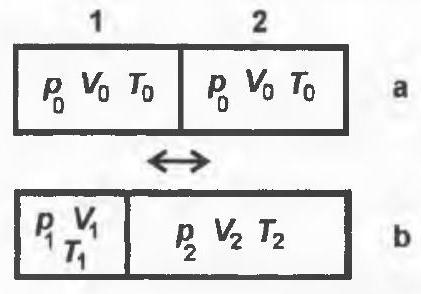
\includegraphics[max width=\textwidth, center]{2025_07_01_5b3ff9fa0d508c8e9f17g-324}\\ Fig. prob. 2.249 \end{center}\\

2.250. Ecuația transformării izoterme\\ $\left(p_{0}+\rho g H\right) V_{0}=\left(p_{0}+\rho g h\right) \frac{4 \pi r^{3}}{3} ; \quad r=\sqrt[3]{\frac{3\left(p_{0}+\rho g H\right) V_{0}}{4 \pi\left(p_{0}+\rho g h\right)}}$\\

2.251. Panta $m$ a dreptei care prin 2 stări oarecare\\ $p_{1}, V_{1}, T_{1}$ si $p_{2}, V_{2}, T_{2}$ de pe dreapta 1 este $m_{1}=\frac{V_{2}-V_{1}}{T_{2}-T_{1}}$. Din ecuația de stare $p_{1} V_{1}=\nu R T_{1}, p_{1} V_{2}=\nu R T_{2}, p_{1} \Delta V=\nu R \Delta T, m_{1}=\frac{\Delta V}{\Delta T}=\frac{\nu R}{p_{1}}$.\\ Din figură se observă $m_{1}<m_{2}<m_{3}$.\\ Pantele $m_{i}(i=1,2,3)$ sunt invers proporționale cu presiunile $p_{3}<p_{2}<p_{1}$.\\

2.252. Corpul 2 cedează căldură. O parte este preluată de corpul 1, iar alta $(Q)$ se pierde în exterior. Astfel, ecuația calorimetrică este:\\ $m_{2} c_{2}\left(t_{2}-t_{f}\right)=m_{1} c_{1}\left(t_{f}-t_{1}\right)+\frac{3}{2} m_{1} c_{1} t_{1}$ sau\\ $\frac{m_{1}}{2} 4 c_{1}\left(2 t_{1}-t_{f}\right)=\frac{1}{2} m_{1} c_{1} t_{1}+m_{1} c_{1} t_{f}$ de unde\\ $t_{f}=\frac{7}{6} t_{1}$\\

2.253. În coordonate $(p, V)$ destinderea gazului ideal se reprezintă printr-o dreaptǎ (vezi Fig. prob. 2.253.). Aria figurii de sub grafic reprezintă tocmai lucrul mecanic efectuat în timpul transformării:\\ $L=\frac{\left(p_{1}+p_{2}\right)\left(V_{1}-V_{2}\right)}{2}$\\ Dar $V_{2}=n V_{1}$ iar $p_{2}=\alpha V_{2}=n \alpha V_{1}$, deci\\ $L=\frac{\left(p_{1}+n \alpha V_{1}\right)(n-1) V_{1}}{2}$\\ Din $p_{1}=\alpha V_{1} \Rightarrow \alpha=\frac{p_{1}}{V_{1}}$ şi $L=\frac{n^{2}-1}{2} p_{1} V_{1}=40 \mathrm{~kJ}$.\\ \begin{center} 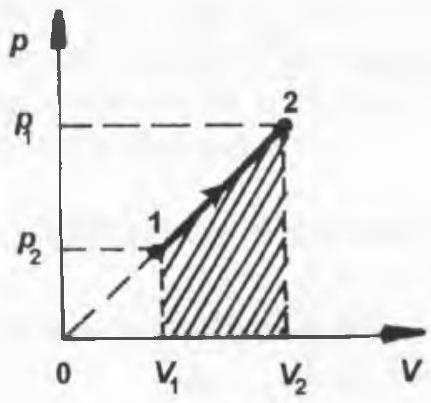
\includegraphics[max width=\textwidth, center]{2025_07_01_5b3ff9fa0d508c8e9f17g-325(1)}\\ Fig. prob. 2.253 \end{center}\\

2.254. Randamentul ciclului este:\\ $\eta=1-\frac{\left|Q_{\text{ced}}\right|}{Q_{\text{abs}}}=1-\frac{\left|Q_{C A}\right|}{Q_{A B}}=1-\frac{\nu R T_{A} \ln \frac{V_{C}}{V_{A}}}{\nu C_{p}\left(T_{B}-T_{A}\right)}=1-\frac{\gamma-1}{\gamma(e-1)} \ln \frac{V_{C}}{V_{A}}$\\ Din ecuația transformărilor:\\ $\mathrm{BC}: T_{B} V_{B}^{\gamma-1}=T_{A} V_{C}^{\gamma-1}, \quad \mathrm{AB}: \frac{V_{A}}{T_{A}}=\frac{V_{B}}{T_{B}} \text { cu } T_{B}=e T_{A}$.\\ Rezultă $\frac{V_{C}}{V_{A}} e^{\frac{\gamma}{\gamma-1}}$ sau $\ln \frac{V_{C}}{V_{A}}=\frac{\gamma}{\gamma-1}$ şi\\ $\eta=\frac{e-2}{e-1}=0,42$.\\

2.255. În coordonate ( $p, T$ ), transformarea izocoră este o dreaptă ce trece prin origine: $p=\frac{\nu R}{V} T$, coeficientul $\frac{\nu R}{V}$ este egal cu panta acestei drepte. Astfel, valoarea maximă a volumului corespunde stării pentru care panta este minimă, adică pentru transformarea $O D$.\\

2.256. În coordonate $(p, V)$ transformarea $1 \rightarrow 2$ este o dreaptă. (Fig. prob. 2.256.)\\ $C=\frac{Q}{\nu\left(T_{2}-T_{1}\right)}=\frac{\Delta U+L}{\nu\left(T_{2}-T_{1}\right)}$\\ Dar $\quad \Delta U=\nu C_{v}\left(T_{2}-T_{1}\right)$\\ $L=\operatorname{aria}\left(12 V_{2} V_{1}\right)=\frac{1}{2}\left(p_{1}+p_{2}\right)\left(V_{2}-V_{1}\right)=\frac{1}{2}\left[\alpha\left(V_{2}+V_{1}\right)+2 \beta\right]\left(V_{2}-V_{1}\right)$, iar\\ $T_{2}-T_{1}=\frac{p_{2} V_{2}-p_{1} V_{1}}{\nu R}=\frac{V_{2}-V_{1}}{\nu R}\left[\alpha\left(V_{2}+V_{1}\right)+\beta\right]$\\ Deci $C=C_{V}+\frac{3 R}{5}=1,6 C_{V}$.\\ \begin{center} 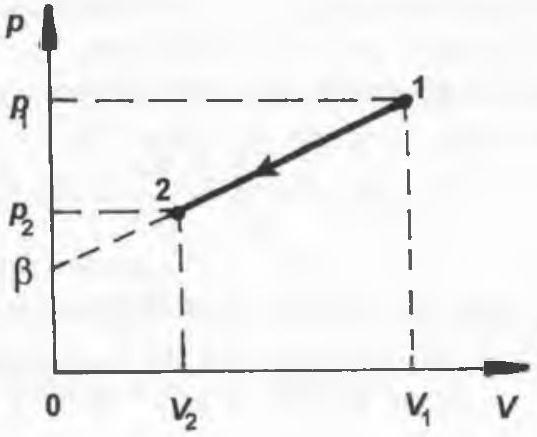
\includegraphics[max width=\textwidth, center]{2025_07_01_5b3ff9fa0d508c8e9f17g-325}\\ Fig. prob. 2.256 \end{center}\\

2.257. $Q_{\text {cedat }}=Q_{\text {ambiant }}$ adică\\ $m_{1} c_{a}\left(\theta-t_{1}\right)=m_{2} c_{a}\left(t_{2}-\theta\right)$ de unde $\theta=12,5^{\circ} \mathrm{C}$\\

2.258. Conform Fig. prob. 2.258 lucrul mecanic este egal cu aria trapezului $V_{1} 12 n V_{1}$,\\ $L=\frac{n p_{1}+p_{1}}{2}\left(n V_{1}-V_{1}\right)=\frac{n^{2}-1}{2} p_{1} V_{1}=36 \mathrm{~kJ}$\\ \begin{center} 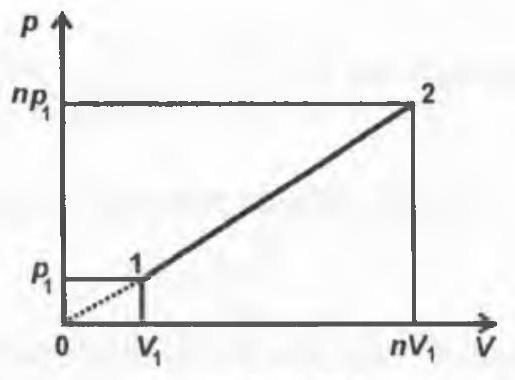
\includegraphics[max width=\textwidth, center]{2025_07_01_5b3ff9fa0d508c8e9f17g-326}\\ Fig. prob. 2.258 \end{center}\\

2.259. Scriind conservarea numărului de moli:\\ $\frac{p V_{1}}{R T}+\frac{p n V_{1}}{R T}=\frac{p_{1} V_{1}}{R k T}+\frac{p_{1} n V_{1}}{R T}$, \\ rezultă raportul\\ $\frac{p_{1}}{p}=\frac{k(n+1)}{1+n k}=\frac{8}{7}$\\

2.260. Randamentul,\\ $=1-\frac{\gamma+(\gamma-1) \ln \frac{V_{1}}{V_{2}}}{\gamma+2(\gamma-1) \ln \frac{V_{4}}{V_{3}}}$, unde $p_{1} V_{1}=p_{2} V_{2}$ şi $p_{1} V_{4}=p_{2} V_{3}$,\\ deci, $\frac{V_{1}}{V_{2}}=\frac{V_{4}}{V_{3}}=\frac{p_{2}}{p_{1}}=e$. Deci, $\eta=\frac{\gamma-1}{3 \gamma-2}=\frac{2}{11}$, de unde $\gamma=\frac{7}{5}$.\\

2.261. Raportul vitezelor este $\frac{\nu_{T, \mathrm{O}_{2}}}{\nu_{T, \mathrm{~N}_{2}}}=\frac{\sqrt{\frac{3 R T}{\mu_{\mathrm{O}_{2}}}}}{\sqrt{\frac{3 R T}{\mu_{\mathrm{N}_{2}}}}}=\frac{\sqrt{\mu_{\mathrm{N}_{2}}}}{\sqrt{\mu_{\mathrm{O}_{2}}}}=\sqrt{\frac{7}{8}}$.\\

2.262. $\Delta \rho=\rho_{2}-\rho_{1}=\frac{m}{V_{1}}-\frac{m}{V_{2}}=40 \mathrm{~kg} / \mathrm{m}^{3}$.\\

2.263. Conform enunţului, $p_{1} V_{\min }=\nu R T_{1}$, de unde $T_{1}=\frac{p_{1} V_{\min }}{v R}$. Dar, randamentul $\eta=\frac{L}{Q_{1}}=\frac{L}{L+\left|Q_{2}\right|}=1-\frac{T_{2}}{T_{1}}$, adică $\left|Q_{2}\right|=\frac{\nu R T_{2} L}{p_{1} V_{\text {min }}-\nu R T_{2}}=80 \mathrm{~kJ}$.\\

2.264. Căldura cedată de Soare în unitatea de timp este\\ $\frac{Q_{\text{ced}}}{\Delta t}=P S$\\ unde $P$ este puterea primită de la Soare pe unitatea de suprafață şi\\ $S$ este suprafata pe care cade energia solară, perpendiculară pe direcția de propagare a emisiei solare.\\ Această căldură este absorbită de apa din tub. În intervalul de timp $\Delta t$, va fi încălzită o masă de apă $\Delta m$ cu $\Delta T$ grade;\\ $Q_{\tetx{abs}}=\Delta m \cdot c \Delta T$\\ Din conservarea energiei rezultă\\ $\Delta m \cdot c \Delta T=P S \Delta t$\\ $\frac{\Delta m}{\Delta t}=\frac{P S}{\Delta T}=\frac{4 \cdot 10^{3} \mathrm{~W}}{4,18 \cdot 10^{3} \mathrm{~J} / \mathrm{KgK} \cdot 40 \mathrm{~K}}=\frac{1}{41,8} \frac{\mathrm{~kg}}{\mathrm{~s}}=1,4 \mathrm{~kg} / \mathrm{minut}$\\ Debitul volumic va fi $\frac{\Delta V}{\Delta t}=1,4 \mathrm{litru} / \mathrm{min}$.\\ 

2.265 $H_{0}=$ presiunea atmosferică\\ $p_{0}=$ presiunea din cilindru după scufundare\\ Inițial, aerul din cilindru se află la presiunea atmosferică $H_{0}$ și ocupă tot\\ volumul cilindrului $V_{0}=h_{1} \pi \frac{D^{2}}{4}$.\\ Aerul rămas în cilindru va ocupa, după scufundare volumul\\ $V_{0}=\left(h_{1}-x\right) \pi \frac{D^{2}}{4}$\\ şi se va afla la presiunea $p_{0}$.\\ Prin scufundare, aerul suferă o transformare izotermă,\\ $H_{0} V_{0}=p_{0} V$\\ $H_{0} h_{1} \pi \frac{D^{2}}{4}=p_{0}\left(h_{1}-x\right) \pi \frac{D^{2}}{4}$\\ La nivelul AB apa este în echilibru, adică\\ $p_{0}=H_{0}+\rho g h$\\ $\Rightarrow H_{0} h_{1}=\left(H_{0}+\rho g h\right)\left(h_{1}-x\right)$\\ $\Rightarrow x=\frac{\rho g h}{H_{0}+\rho g h} h_{1}=\frac{h_{1}}{1+\frac{H_{0}}{\rho g h}}=1,18 \mathrm{~m}$\\ \begin{center} 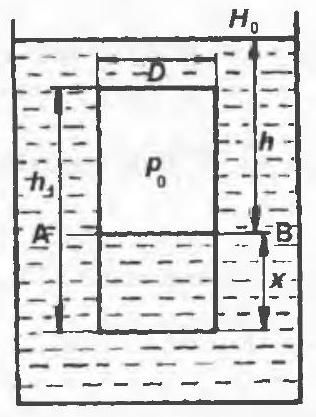
\includegraphics[max width=\textwidth, center]{2025_07_01_5b3ff9fa0d508c8e9f17g-328}\\ Fig. prob. 2.265 \end{center}\\

2.266. O masă $m$ de aer conține:\\ $0,7554 \mathrm{~m}$ azot\\ $0,231 \mathrm{~m}$ oxygen\\ $0,013 \mathrm{~m}$ argon.\\ Numărul de moli de aer conținuți în masa $m$ este:\\ $\nu_{\text{aer}}=\nu_{\mathrm{N}_{2}}+\nu_{\mathrm{O}_{2}}+\nu_{\mathrm{Ar}}$\\ Tinând cont că $\nu=\frac{m}{\mu}$, rezultă\\ $\frac{m}{\mu_{a e r}}=\frac{0,7554 \mathrm{~m}}{\mu_{\mathrm{N}_{2}}}+\frac{0,231 \mathrm{~m}}{\mu_{\mathrm{O}_{2}}}+\frac{0,013 \mathrm{~m}}{\mu_{\mathrm{Ar}}}$\\ $\Rightarrow \frac{1}{\mu_{a e r}}=\frac{0,7554}{\mu_{\mathrm{N}_{2}}}+\frac{0,231}{\mu_{\mathrm{O}_{2}}}+\frac{0,013}{\mu_{\mathrm{Ar}}}$\\ unde: $\mu_{\mathrm{N}_{2}}=28 \mathrm{~g} / \mathrm{mol} ; \mu_{\mathrm{O}_{2}}=32 \mathrm{~g} / \mathrm{mol} ; \mu_{\mathrm{Ar}}=40 \mathrm{~g} / \mathrm{mol}$, molecule biatomice\\ $\Rightarrow \mu_{a e r}=29 \mathrm{~g} / \mathrm{mol}$\\ 

2.267. Considerând cele două gaze ideale, energia internă este în starea inițială:\\ \begin{center} \begin{tabular}{|c|c|} \hline He & $\mathrm{O}_{2}$ \\ $V_{0}, p_{0}$ & $V_{0}, p_{0}$ \\ $T_{\mathrm{He}}$ & $T_{\mathrm{O}_{2}}$ \\ \hline \end{tabular} \end{center}\\ $U_{\mathrm{He}}=\frac{3}{2} N_{\mathrm{He}} k T_{\mathrm{He}} \quad$ (monoatomic)\\ $U_{\mathrm{O}_{2}}=\frac{5}{2} N_{\mathrm{O}_{2}} k T_{\mathrm{O}_{2}} \quad$ (biatomic)\\ După amestecare, gazele vor avea aceeaşi temperatură $T$. Din conservarea energiei rezultă:\\ $\Delta U_{\mathrm{O}_{2}}=\Delta U_{\mathrm{He}}$\\ $\frac{3}{2} N_{\mathrm{He}} k\left(T-T_{\mathrm{He}}\right)=\frac{5}{2} N_{\mathrm{O}_{2}} k\left(T_{\mathrm{O}_{2}}-T\right)$\\ unde:\\ $p_{0} V_{0}=N_{\mathrm{He}} k T_{\mathrm{He}} \Rightarrow N_{\mathrm{He}}=\frac{p_{0} V_{0}}{k T_{\mathrm{He}}}$\\ $p_{0} V_{0}=N_{\mathrm{O}_{2}} k T_{\mathrm{O}_{2}} \Rightarrow N_{\mathrm{O}_{2}}=\frac{p_{0} V_{0}}{k T_{\mathrm{O}_{2}}}$\\ $\frac{3}{2} \frac{p_{0} T_{0}}{k T_{\mathrm{He}}} k\left(T-T_{\mathrm{He}}\right)=\frac{5}{2} \frac{p_{0} T_{0}}{k T_{\mathrm{O}_{2}}} k\left(T_{\mathrm{O}_{2}}-T\right)$\\ $3 \frac{T}{T_{\mathrm{He}}}-3=5-5 \frac{T}{T_{\mathrm{O}_{2}}} \Rightarrow T=\frac{8 T_{\mathrm{He}} T_{\mathrm{O}_{2}}}{3 T_{\mathrm{O}_{2}}+5 T_{\mathrm{He}}} \text { şi } T=284 \mathrm{~K}$\\

2.268. Bilanţul căldurii schimbate între calorimetru, apă şi cupru, în cursul atingerii echilibrului termic, se scrie:\\ $\left(m_{C} c_{\mathrm{Cu}}+m_{a} c_{a}\right)\left(t_{f}-t_{1}\right)=m_{\mathrm{Cu}} c_{\mathrm{Cu}}\left(t_{2}-t_{f}\right)$\\ de unde:\\ $c_{\mathrm{Cu}}=\frac{m_{a} c_{a}\left(t_{f}-t_{1}\right)}{m_{\mathrm{Cu}}\left(t_{2}-t_{f}\right)-m_{C}\left(t_{f}-t_{1}\right)} \cong 381 \mathrm{~J} / \mathrm{kg}$.\\

2.269. Randamentul ciclului Carnot este: $\eta=1-\frac{\left|Q_{2}\right|}{Q_{1}}=1-\frac{T_{2}}{T_{1}}$ întrucât: $\frac{\left|Q_{2}\right|}{Q_{1}}=\frac{T_{2}}{T_{1}}$. Astfel, $T_{2}=T_{1} \frac{\left|Q_{2}\right|}{Q_{1}}=400 \cdot \frac{320}{400}=320 \mathrm{~K}$, iar randamentul este:\\ $\eta=1-\frac{320}{400}=20 \%$\\

2.270. Viteza termică a moleculelor gazului ideal este dată de formula:\\ $v_{T}=\sqrt{\frac{3 R T}{\mu}}$.\\ Egalitate între vitezele termice se obține aşadar când:\\ $\frac{T_{\mathrm{O}_{2}}}{\mu_{\mathrm{O}_{2}}}=\frac{T_{\mathrm{H}_{2}}}{\mu_{\mathrm{H}_{2}}}=\frac{273}{2}$\\ de unde $T_{\mathrm{O}_{2}} \approx 4097^{\circ} \mathrm{C}$.\\

2.271. Principiul I al termodinamicii se exprimă cantitativ prin ecuația:\\ $Q=\Delta U+L$\\

2.272. În decursul unui proces ciclic monoterm ireversibil, sistemul trebuie să primească lucru mecanic (formularea Thomson a principiului al II-lea al termodinamicii). Prin urmare $Q \neq L<0$.\\

2.273. Într-o transformare reversibilă izotermă, lucrul mecanic efectuat de gazul ideal este:\\ $L=\nu R T \ln \frac{V_{2}}{V_{1}}$\\ relație care devine, ținând cont de legea Boyle-Mariotte $p_{1} V_{1}=p_{2} V_{2}$,\\ $L=\nu R T \ln \frac{p_{1}}{p_{2}}$\\

2.274. Transformarea $1 \rightarrow 2$ :\\ $V=\mathrm{ct} \Rightarrow L=0$\\ $T_{2}>T_{1} \Rightarrow$ sistemul primeşte căldură $Q_{12}=\nu C_{V}\left(T_{2}-T_{1}\right)$.\\ Transformarea $2 \rightarrow 3$ :\\ $T=\mathrm{ct}, V_{3}>V_{2}, Q_{23}=L_{23}$\\ $\Rightarrow$ sistemul primeşte căldură\\ $Q_{23}=\nu R T_{2} \ln \frac{V_{2}}{V_{1}}$\\ Transformarea $3 \rightarrow 4: V=\mathrm{ct}, T_{2}>T_{1}, L=0 \Rightarrow$ sistemul cedează căldură\\ $Q_{34}=\nu C_{V}\left(T_{1}-T_{2}\right)$\\ Transformarea $4 \rightarrow 1: T=\mathrm{ct}, Q_{41}=L_{41} \Rightarrow$ sistemul cedează căldură\\ $Q_{41}=\nu R T_{1} \ln \frac{V_{1}}{V_{2}}$\\ Randamentul acestui ciclu este:\\ $\eta=\frac{Q_{12}+Q_{23}+Q_{34}+Q_{41}}{Q_{12}+Q_{23}}=\frac{\nu R T_{2} \ln \frac{V_{2}}{V_{1}}+\nu R T_{1} \ln \frac{V_{1}}{V_{2}}}{\nu C_{V}\left(T_{2}-T_{1}\right)+\nu R T_{2} \ln \frac{V_{2}}{V_{1}}}$.\\ $\eta=\frac{R\left(T_{2}-T_{1}\right) \ln \frac{V_{2}}{V_{1}}}{C_{V}\left(T_{2}-T_{1}\right)+R T_{2} \ln \frac{V_{2}}{V_{1}}} $.\\ \begin{center} 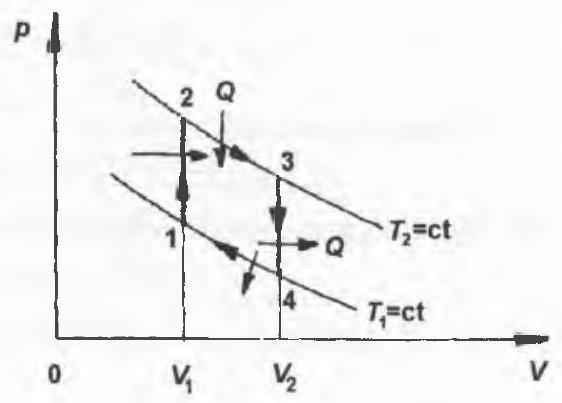
\includegraphics[max width=\textwidth]{2025_07_01_5b3ff9fa0d508c8e9f17g-330}\\ Fig. prob. 2.274 \end{center}\\

2.275. Cunoscând faptul că energia internă este o mǎrime aditivă avem:\\ $U_{\mathrm{in}}=\nu C_{V} T_{1}+\nu C_{V} T_{2}$ (1)\\ $U_{\mathrm{fin}}=\nu_{1} C_{V} T_{\mathrm{fin}}+\nu_{2} C_{V} T_{\mathrm{fin}}$ (2)\\ unde: $\quad T_{\text {fin }}$ - temperatura finală de echilibru\\ $\nu_{1}, \nu_{2}$ - numărul de moli final din cele două vase.\\ Pentru că cele două vase sunt izolate adiabatic avem pentru sistemul total $Q=0$ şi $L=0$. Astfel, conform principiului întâi al termodinamicii:\\ $\Delta U=0$, deci energia internă a sistemului se conservă.\\ Astfel\\ $U_{\mathrm{in}}=U_{\mathrm{fin}}$ (3)\\ Ținând cont că numărul de moli se conservă în procesul de amestecare, avem:\\ $\nu_{1}+\nu_{2}=2 \nu$ (4)\\ Introducând în relația (3) relațiile (1), (2) şi (4) se va obține:\\ $T_{\text {fin }}=\frac{T_{1}+T_{2}}{2}$\\ Ecuația generală a gazelor\\ $p_{\text {fin }}\left(V_{1}+V_{2}\right)=2 \nu R T_{\text {fin }}$\\ în care am ținut cont de relația (4) conduce la:\\ $p_{f i n}=\frac{\nu R T_{1}+\nu R T_{2}}{V_{1}+V_{2}}=\frac{p V_{1}+p V_{2}}{V_{1}+V_{2}}=p$\\

2.276. a) Procesul fiind lent, are loc echilibrarea temperaturii şi procesul va fi izoterm.\\ Deci $T_{1}=T_{2}=300 \mathrm{~K}$.\\ Aplicând legea lui Boyle-Mariotte se găseşte:\\ $p_{1} V_{1}=p_{2} V_{2}$\\ $V_{2}=5 \mathrm{~litri}$.\\ b) Pentru că procesul este rapid, nu are loc schimb de căldură şi va fi un proces adiabatic.\\ Deci\\ $p_{1} V_{1}^{\gamma}=p_{2} V_{2}^{\gamma} \Rightarrow V_{2}^{\gamma}=\frac{p_{1}}{p_{2}} V_{1}^{\gamma}=\frac{V_{1}^{\gamma}}{2}=\frac{10^{1,4}}{2} \Rightarrow V_{2}=6,1 \mathrm{~litri}$.\\ Noua temperatură va fi: $\quad \frac{p_{1} V_{1}}{T_{1}}=\frac{p_{2} V_{2}}{T_{2}} \Rightarrow T_{2}=366 \mathrm{~K}$.\\

2.277. $p=\frac{F_{e}}{S}=\frac{k h}{S}$\\ $p_{1}=\frac{F_{e}}{S}=\frac{k h_{1}}{S}$\\ $\frac{p V}{T}=\frac{p_{1} V_{1}}{T_{1}} ; \frac{k h h S}{T}=\frac{k h_{1} S h_{1}}{T_{1}} \Rightarrow \frac{h^{2}}{T}=\frac{h_{1}^{2}}{T_{1}} \Rightarrow h_{1}=h \sqrt{\frac{T_{1}}{T}} .$\\ \begin{center} 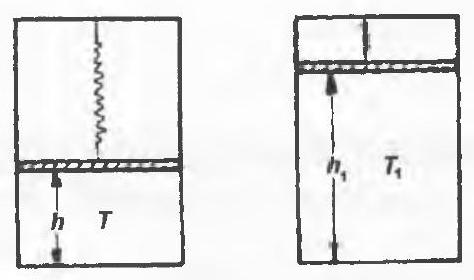
\includegraphics[max width=\textwidth, center]{2025_07_01_5b3ff9fa0d508c8e9f17g-332}\\ Fig. prob. 2.277 \end{center}\\

2.278. $\quad \eta\left(\frac{m v_{i}^{2}}{2}-\frac{m v_{f}^{2}}{2}\right)=m c \Delta T$.\\ Se obține:\\ $\Delta T=\frac{1}{2 c}\left(v_{1}^{2}-v_{f}^{2}\right) \cong 6,5 \mathrm{~K}$\\

2.279. $\begin{array}{ll} m=m_{\mathrm{O}_{2}}+m_{\mathrm{N}_{2}}\\ N=N_{\mathrm{O}_{2}}+N_{\mathrm{N}_{2}} & \mu=\frac{N_{\mathrm{O}_{2}} \mu_{\mathrm{O}_{2}}+N_{\mathrm{N}_{2}} \mu_{\mathrm{N}_{2}}}{N_{\mathrm{O}_{2}}+N_{\mathrm{N}_{2}}} \\ m_{\mathrm{O}_{2}}=N_{\mathrm{O}_{2}} \mu_{\mathrm{O}_{2}}\\ m_{\mathrm{N}_{2}}=N_{\mathrm{N}_{2}} \mu_{\mathrm{N}_{2}} & m_{\mathrm{O}_{2}}=m_{\mathrm{N}_{2}} \frac{\mu-\mu_{\mathrm{N}_{2}}}{\mu_{\mathrm{O}_{2}}-\mu} \frac{\mu_{\mathrm{O}_{2}}}{\mu_{\mathrm{N}_{2}}}=16 \mathrm{~g} \end{array}$\\

2.280. $v_{t}=\sqrt{\frac{3 R T}{\mu}}=\sqrt{3 \frac{P}{\rho}} \Rightarrow P=\frac{v_{t}^{2} \rho}{3}=1,5 \cdot 10^{6} \mathrm{Nm}^{-2}=1,5 \mathrm{MNm}^{-2}$.\\

2.281. Proces izocor $\frac{p}{p_{i}}=\frac{T}{T_{i}} \Rightarrow p=p_{i}+\frac{F}{S}$;\\ $T=T_{i} \frac{p}{p_{i}}=\frac{p_{i} S+F}{p_{i} S} T_{i}=350 \mathrm{~K}$\\

2.282. Numărul de molecule rămâne constant:\\ $M=\nu \cdot N_{A}=6,023 \cdot 10^{23} \cdot 10^{3} \cdot 1,5=$\\ $=6,023 \cdot 10^{26} \text { molecule } / \mathrm{kmol} \cdot 1,5 \mathrm{kmol}=9 \cdot 10^{26}$ molecule\\

2.283. Căldura este folosită pentru schimbarea de fază. $d=12 \mathrm{~g} / \mathrm{min}$ este debitul de benzină consumat.\\ $m_{v} \lambda_{v}=\eta Q_{b} d \tau$\\ $\frac{\Delta m_{a}}{\Delta t}=-\frac{m_{v}}{\tau}=\frac{-\eta Q_{b} d}{\lambda_{v}}=-3 \mathrm{~g} / \mathrm{s}$\\

2.284. Varianta 1\\ Utilizăm primul principiu al termodinamicii $\Delta U=Q-L$ in care $Q=\nu C_{p}\left(T_{2}-T_{1}\right)$, iar temperatura $T_{2}$ o exprimăm din ecuația de stare $T_{2}=\frac{\mu p_{2} V_{2}}{m R}$, iar lucrul mecanic pentru o transformare izobară este:\\ $L=p\left(V_{2}-V_{1}\right)=p V_{2}-\frac{m}{\mu} R T_{1}$\\ şi obținem variația de energie internă\\ $\Delta U=\frac{m}{\mu} C_{p}\left(\frac{\mu p V_{2}}{m R}-T_{1}\right)-p V_{2}+\frac{m}{\mu} R T_{1}$\\ sau $\Delta U=\frac{5}{2}\left(p V_{2}-\frac{m}{\mu} R T_{1}\right)$.\\ Varianta 2\\ Folosim definiția variației energiei interne $\Delta U=\nu C_{v}\left(T_{2}-T_{1}\right)$ şi relația lui Mayer $C_{p}-C_{v}=R$ obținem $\Delta U=\frac{5}{2}\left(p V_{2}-\frac{m}{\mu} R T_{1}\right)$\\ Introducând mărimile cunoscute obținem: $\quad \Delta U=1126,25 \mathrm{~J}$.\\ 

2.285. Căldura cedată de aer este $|Q|=\nu C_{v}\left(T_{1}-T_{2}\right)$, iar ecuațiile de stare sunt $p_{1} V=\nu R T_{1}$, respectiv $p_{2} V=\nu R T_{2}$. Inlocuind temperaturile $T_{1}$ și $T_{2}$ în căldura cedată obținem:\\ $|Q|=\nu \frac{5}{2} R\left(\frac{p_{1} V}{\nu R}-\frac{p_{2} V}{\nu R}\right) \Rightarrow|Q|=\frac{5}{2}\left(p_{1}-p_{2}\right) V$\\ de unde putem determina presiunea $p_{2}=p_{1}-\frac{2}{5} \frac{Q}{V}$.\\ Înlocuind valorile numerice obținem:\\ $p_{2}=3 \cdot 10^{5} \mathrm{~N} / \mathrm{m}^{2}$\\

2.286. Din definiţia randamentului unei maşini termice cunoaştem $\eta=1-\frac{\left|Q_{2}\right|}{Q_{1}}$, iar pentru randamentul unui ciclu Carnot: $\quad \eta=1-\frac{T_{2}}{T_{1}}$\\ Egalând cele două expresii ale randamentului putem determina căldura cedată sursei reci.\\ $\left|Q_{2}\right|=Q_{1} \frac{T_{2}}{T_{1}}=1500 \mathrm{~J}$\\

2.287. Energia cinetică a moleculelor din vas se transformă în energie termică\\ $\frac{m v^{2}}{2}=m c_{v} \Delta t \Rightarrow \Delta t=\frac{v^{2}}{2 c_{v}} \Rightarrow t_{2}=t_{1}+\frac{v^{2}}{2 c_{v}}=24^{\circ} \mathrm{C}$\\

2.288. Ecuațiile de stare ce descriu cele două situații sunt:\\ $p V=\frac{m}{\mu} R T_{1} ; \quad p V=\frac{(m-\Delta m)}{\mu} R T_{2}$\\ Eliminând $p V \Rightarrow \frac{m}{\mu} R T_{1}=\frac{(m-\Delta m)}{\mu} R T_{2}$ sau $m\left(T_{2}-T_{1}\right)=\Delta m T_{2}$\\ $\Delta m=m \frac{\left(T_{2}-T_{1}\right)}{T_{2}}$\\ în care înlocuim $m$ din prima ecuație de stare:\\ $\Delta m=\frac{\mu p V}{R T_{1}} \frac{T_{2}-T_{1}}{T_{2}}=1,45 \cdot 10^{-3} \mathrm{~kg}$\\

2.289. Debitul volumic este dat de $Q=\frac{V}{t}=S \cdot v \Rightarrow v=\frac{V}{S \cdot t}$, dar $V=\frac{m}{\rho}$ şi $p V=\frac{m}{\mu} R T$ sau $p=\frac{\rho}{\mu} R T$. Înlocuind in expresia vitezei obținem:\\ $v=\frac{m R T}{p \mu t S}=10,3 \mathrm{~m} / \mathrm{s}$\\

2.290. $\quad \eta=1-\frac{\left|Q_{c}\right|}{Q_{\text{abs}}} ; \quad Q_{\text{abs}}=Q_{12}=\nu C_{p}\left(T_{2}-T_{1}\right) ; \quad \gamma=\frac{C_{p}}{C_{v}}=\frac{C_{v}+R}{C_{v}}$ de unde $\quad C_{v}=\frac{R}{\gamma-1}=\frac{3}{2} R, C_{p}=\frac{5}{2} R$\\ $Q_{12}=\nu \frac{5}{2} R\left(4 T_{1}-T_{1}\right)=\frac{15 \nu R T_{1}}{2}>0$\\ deoarece: $\quad \frac{T_{2}}{T_{1}}=\frac{V_{2}}{V_{1}}=4 \Rightarrow T_{2}=4 T_{1}$\\ $Q_{c}=Q_{23}+Q_{31}$\\ $Q_{23}=\nu C_{v}\left(T_{3}-T_{2}\right)$\\ deoarece: $\quad \frac{T_{2}}{T_{3}}=\frac{p_{2}}{p_{1}}=2 \Rightarrow T_{3}=\frac{T_{2}}{2}=2 T_{1}$ avem:\\ $Q_{23}=\nu \frac{3 R}{2}\left(2 T_{1}-4 T_{1}\right)=-3 \nu R T_{1}=-6 p_{1} V_{1}$\\ $Q_{31}=\Delta U_{31}-L_{31}=\nu C_{v}\left(T_{1}-T_{3}\right)-L_{31}$\\ unde:\\ $L_{31}=\frac{2 p_{1}+p_{1}}{2} \cdot 3 p_{1}=\frac{9 p_{1} V_{1}}{2}$\\ iar\\ $Q_{31} =\nu C_{v}\left(T_{1}-T_{3}\right)-\frac{9 p_{1} V_{1}}{2}=\frac{3 R}{2}\left(-T_{1}\right)-\frac{9 p_{1} V_{1}}{2}= $\\ $=-\frac{3}{2} 2 p_{1} V_{1}-\frac{9 p_{1} V_{1}}{2}=-\frac{15 p_{1} V_{1}}{2}<0$\\ Randamentul ciclului este:\\ $\eta=1-\frac{6 p_{1} V_{1}+\frac{15 p_{1} V_{1}}{2}}{15 p_{1} V_{1}}=0,1=10 \%$.\\

2.291. $\Delta U=\nu C_{v} \Delta T=\nu \frac{5 R}{2}\left(T_{2}-T_{1}\right)$\\ $T_{2}=a V_{2}-b V_{2}^{2}=a n V_{1}-b n^{2} V_{1}^{2}$\\ $\quad p_{1} V_{1}=\nu R T_{1} \text { de unde } V_{1}=\frac{\nu R T_{1}}{p_{1}}$.\\ Rezultă\\ $T_{2}=n V_{1}\left(a-b n V_{1}\right)=\frac{n \nu R T_{1}}{p_{1}}\left(a-b n \frac{\nu R T_{1}}{p_{1}}\right)$\\ $\Delta U =\nu \frac{5 R}{2}\left[n \frac{\nu R T_{1}}{p_{1}}\left(a-b n \frac{\nu R T_{1}}{p_{1}}\right)-T_{1}\right]=$\\ $=\frac{5}{2} \nu R T_{1}\left[n \frac{\nu R}{p_{1}}\left(a-b n \frac{\nu R T_{1}}{p_{1}}\right)-1\right]$.\\ Se obține:\\ $\Delta U =\frac{5 \nu R}{2}\left(a n V_{1}-b n^{2} V_{1}^{2}-a V_{1}+b V_{1}^{2}\right)=$\\ $=\frac{5 \nu R V_{1}}{2}\left[a(n-1)-b V_{1}\left(n^{2}-1\right)\right]=$\\ $=\frac{5 \nu R V_{1}(n-1)}{2}\left[a-b V_{1}(n+1)\right]$.\\

2.292. Din ecuația termică de stare $p V=\nu R T$, obținem $p=\nu R a+\nu R b V$.\\ Lucrul mecanic este dat de relația\\ $L =\int_{V_{1}}^{V_{2}} p \mathrm{~d} V=\int_{V_{1}}^{V_{2}}(R a+R b V) \mathrm{d} V=$ \\ $=4 R V_{1}\left(a+3 b V_{1}\right)$.\\

2.293. Capacitatea caloricã molară la volum constant este $C_{v}=\frac{R}{\gamma-1}$ iar căldura specifică la volum constant este $c_{v}=\frac{C_{v}}{\mu}=\frac{R}{\mu}=\frac{R}{\mu(\gamma-1)}$. Densitatea gazului în conditii normale este $\rho_{0}=\frac{p_{0} \mu}{R T_{0}}$, de unde rezultǎ $c_{v}=\frac{p_{0}}{\rho_{0} T_{0}(\gamma-1)}$, deci $\gamma=1+\frac{p_{0}}{\rho_{0} T_{0} c_{v}} ;$\\

2.294. La volum constant $\frac{p}{T}=$ const., deci temperatura gazului va creşte de 2 ori: $\quad v_{t}=\sqrt{\frac{3 R T}{\mu}} \sim \sqrt{T}$, deci viteza termică va creşte de $\sqrt{2}$.\\

2.295. Densitatea unui gaz are expresia $\rho=\frac{p \mu}{R T}=a \cdot p$, cu $a=\frac{\mu}{R T}$. Pentru ca $a$ să fie constantă trebuie ca $T=$ const.\\

2.296. Ecuația de stare a amestecului în starea inițială:\\ $p V=\left(\frac{m_{H e}}{\mu_{H e}}+\frac{m_{H_{2}}}{\mu_{H_{2}}}\right) R T$\\ În starea finală: $1,2 p V=\left(\frac{2 m_{H e}}{\mu_{H e}}+\frac{m_{H_{2}}}{\mu_{H_{2}}}\right) R T$. Împărțind cele două, se obține în final $\frac{m_{H e}}{m_{H e}}=\frac{1}{2}=0,5$.\\

2.297. Randamentul ciclului Carnot $\eta_{c}=1-\frac{T_{\text {rece }}}{T_{\text {cald }}}=1-\frac{T}{3 T}=\frac{2}{3}$. Pe de $\eta_{c}=\frac{L}{Q_{a b s}}$. Ştiind că se absoarbe caldură absorbită este egală cu lucrul mecanic efectuat $\left(Q_{o b s}=L_{1}\right)$, se obține $\eta_{c}=\frac{L}{L_{1}}=\frac{2}{3}$, de unde $L_{1}=\frac{3 L}{2}=1350 \mathrm{~J}=1,35 \mathrm{~kJ}$.\\

% fig 2.46. nu exista
2.298. $\eta=1-\frac{\left|Q_{c e d}\right|}{Q_{a b s}}$ Gazul absoarbe căldură în transformarea $1-2$ şi cedează în transformarea 3-1 (fig. 2.46). $\eta=1-\frac{\left|Q_{31}\right|}{Q_{12}}$\\ $Q_{12}=\nu C_{12}\left(T_{2}-T_{1}\right)$, unde $C_{12}$ este capacitatea calorică molară a gazului în transformarea 1-2.\\ $C_{12}=\frac{C_{p}+C_{v}}{2}=\frac{1}{2}\left(\frac{R \gamma}{\gamma-1}+\frac{R}{\gamma-1}\right)=\frac{1}{2} R \frac{\gamma+1}{\gamma-1}=2 R$\\ În starea 2: $p_{2}=a V_{2}=a \cdot 2 V_{1}=2 p_{1}$, iar $T_{2}=\frac{p_{2} V_{2}}{\gamma R}=\frac{2 p_{1} \cdot 2 V_{1}}{\gamma R}=4 T_{1}$. In procesul $3-1,\left|Q_{31}\right|=\gamma C_{p}\left(T_{3}-T_{1}\right)$, cu $C_{p}=\frac{R \gamma}{\gamma-1}=\frac{5 R}{2}$. Pentru aflarea temperaturii în starea 3 folosim ecuația adiabatei sub forma $p \cdot T^{\frac{\gamma}{1-\gamma}}=$ constant, adică $p_{2} T_{2}^{\frac{\gamma}{1-\gamma}}=p_{1} T_{3}^{\frac{\gamma}{1-\gamma}}$, de unde\\ $T_{3}=2^{\frac{1-\gamma}{\gamma}} T_{2}=2^{\frac{1-\gamma}{\gamma}} 2^{2} T_{1}=2^{\frac{1+\gamma}{\gamma}} T_{1}=2^{\frac{8}{5}} T_{1} \cong 3,03 T_{1}$. \\ $\eta=1-\frac{\gamma \cdot \frac{5 R}{2} \cdot 2,03 T_{1}}{\gamma \cdot 2 R \cdot 3 T_{1}}=0,154=15,4 \%$.\\

2.299. Într-un proces izobar $L=p\left(V_{2}-V_{1}\right)=\gamma R\left(T_{2}-T_{1}\right)$ iar $Q=\gamma C_{p}\left(T_{2}-T_{1}\right) \cdot \frac{Q}{L}=\frac{C_{p}}{R}=\frac{2800}{800}$, de unde $C_{p}=\frac{7}{2} R$. Cum $C_{v}=C_{p}-R=\frac{5}{2} R$, exponentul adiabatic va fi $\gamma=\frac{7}{5}$.\\

2.300. $C_{\nu 1}=\frac{3 R}{2} ; C_{\nu 2}=\frac{5 R}{2} ; C_{p 1}=\frac{5 R}{2} ; C_{p 2}=\frac{7 R}{2}$;\\ $C_{V_{\text { amestec }}}=\frac{\nu_{1} C_{v 1}+\nu_{2} C_{v 2}}{\nu_{1}+\nu_{2}} ; \quad C_{P_{\text {amestec }}}=\frac{\nu_{1} C_{p 1}+\nu_{2} C_{p 2}}{\nu_{1}+\nu_{2}}$; \\ $\gamma_{\text {amestec }}=\frac{\nu_{1} C_{p 1}+\nu_{2} C_{p 2}}{\nu_{1} C_{v 1}+\nu_{2} C_{v 2}}=1,47$\\

2.301. În transformarea adiabatică $L=-\Delta U=\nu C_{v}\left(T_{1}-T_{2}\right)$. Notăm raportul cerut $f=\frac{T_{2}}{T_{1}}$, deci $T_{2}=f T_{1}$; cu $C_{v}=\frac{R}{\gamma-1}$, obținem $L=\frac{\nu R T_{1}(1-f)}{\gamma-1}$, de unde\\ $f=1-\frac{(\gamma-1)}{\nu R T_{1}}=1-\frac{(\gamma-1)}{p_{1} V_{1}}=1-\frac{6 \cdot 10^{3} \cdot 0,4}{8 \cdot 10^{5} \cdot 4 \cdot 10^{-3}}=\frac{1}{4}=0,25$.\\

2.302. Transformarea gazului este o politropă ( $C=$ const.), de tipul $p V^{n}=a$, cu indicele $n=\frac{2}{3}$. Relația dintre indicele politropei $n$ şi capacitatea calorică molară este $n=\frac{C-C_{p}}{C-C_{V}}$. Tinând seama că $C_{p}=\gamma \cdot C_{V}$ şi $C_{V}=\frac{R}{\gamma-1}=\frac{5}{2} R$, se obţine $C=\frac{11}{2} R$. Ecuaţia procesului politrop se mai poate scrie: $T V^{n-1}=$ const., adică $T_{1} V^{-1 / 3}=T_{2}(8 V)^{-1 / 3}$, de unde se obține $T_{2}=8^{1 / 3} T_{1}=2 T_{1}=600 \mathrm{~K}$.\\ Atunci căldura schimbată cu exteriorul se scrie:\\ $Q=\nu C\left(T_{2}-T_{1}\right)==\frac{11}{2} R\left(T_{2}-T_{1}\right)=13711,5 \mathrm{~J} \cong 13,7 \mathrm{~kJ}$\\

2.303. Ecuația transformării adiabatice se poate scrie $T p^{\frac{1-\gamma}{\gamma}}=$ const., adică $T_{1} p_{1}{ }^{\frac{1-\gamma}{\gamma}}=T_{2} p_{2}{ }^{\frac{1-\gamma}{\gamma}}$, de unde $\frac{T_{2}}{T_{1}}=\left(\frac{p_{1}}{p_{2}}\right)^{\frac{1-\gamma}{\gamma}}=\left(\frac{p_{2}}{p_{1}}\right)^{\frac{\gamma-1}{\gamma}}=4$;\\ $\nu=\sqrt{\frac{3 R T}{\mu}}$, deci $\frac{\nu_{2}}{\nu_{1}}=\sqrt{\frac{T_{2}}{T_{1}}}=2$.

2.304. $[p]_{S I}=\frac{[F]_{S I}}{[S]_{S I}}=\frac{[m]_{S I} \cdot[a]_{S I}}{[S]_{S I}}=\frac{K g \cdot m \cdot s^{-2}}{m^{2}}=K g \cdot m^{-1} \cdot s^{-2}$\\

2.305. $\gamma=\frac{C_{p}}{C_{v}} \Rightarrow C_{p}=\gamma C_{v}$\\ $C_{p}=C_{v}+R \Rightarrow X_{v}=C_{v}+R \Rightarrow C_{v}=\frac{R}{\gamma-1} ; \quad C_{p}=\chi_{v}=\frac{R \gamma}{\gamma-1}$\\

2.306. $p V=\nu R T \Rightarrow T=\frac{p V}{\nu R}$\\ $V=a T^{-1} \Leftrightarrow V=\frac{a}{T}=\frac{a \nu R}{p V} \Leftrightarrow p V^{2}=a \nu R \Leftrightarrow p V^{2}=$ const $. \Rightarrow n=2$\\ (indicele politropic)\\ Cum $C=C_{v}-\frac{R}{n-1}=\frac{5 R}{2}-R=\frac{3 R}{2}$\\

2.307. $\mathrm{T}(\mathrm{K})=t\left({ }^{\circ} \mathrm{C}\right)+273$\\ $v_{T}=\sqrt{\frac{3 R T}{\mu}} \Rightarrow v_{T_{1}}=\sqrt{\frac{3 R T_{1}}{\mu}}$ şi $v_{T_{2}}=\sqrt{\frac{3 R T_{2}}{\mu}}$\\ $\frac{v_{T_{2}}}{v_{T_{1}}}=\sqrt{\frac{T_{2}}{T_{1}}}=\sqrt{\frac{900 \mathrm{~K}}{300 \mathrm{~K}}}=\sqrt{3}$\\

2.308. $\eta=1-\frac{\left|Q_{c}\right|}{Q_{p}} \Rightarrow\left|Q_{c}\right|=Q_{p}(1-\eta)=1200 \mathrm{~J} \cdot 0,4=480 \mathrm{~J}$\\

2.309. $\rho=\frac{m}{V} ; m=\nu \mu ; \quad p V=\nu R T \Rightarrow V=\frac{\nu R T}{p} ; \rho=\frac{m}{V}=\frac{\mu p}{R T}$.\\

2.310. $\eta=\frac{L}{Q_{p}} \Rightarrow L=\eta Q_{p} ; \eta=1-\frac{\left|Q_{c}\right|}{Q_{p}} \Rightarrow Q_{p}=Q_{c} /(1-\eta)=\frac{210 \mathrm{~J}}{0,7}=300 \mathrm{~J}$\\ $P=n \eta Q_{p}=900 \mathrm{~W}$\\

2.311. $Q=\nu C_{p}\left(T_{2}-T_{1}\right)=\frac{\nu R \gamma}{\gamma-1}\left(T_{2}-T_{1}\right)$\\ $p V=\nu R T \Rightarrow p V_{1}=\nu R T_{1} \quad$ şi $\quad p V_{2}=\nu R T_{2}$\\ $Q=\nu C_{p}\left(T_{2}-T_{1}\right)=\frac{\nu R \gamma}{\gamma-1}\left(T_{2}-T_{1}\right)=\frac{p \gamma}{\gamma-1}\left(V_{2}-V_{1}\right) ; \Rightarrow V_{2}=\frac{Q(\gamma-1)}{p \gamma}+V_{1}$.\\

2.312. Sistemul primeşte căldură în transformările: izocoră (1)-(2) și izobară (2)-(3)\\ $Q_{p}=\nu C_{v}\left(T_{2}-T_{1}\right)+\nu C_{p}\left(T_{3}-T_{2}\right)$\\ în transformarea izocoră (1)-(2) avem: $\frac{p_{1}}{T_{1}}=\frac{p_{2}}{T_{2}} \Rightarrow T_{2}=T_{1} \frac{p_{2}}{p_{1}}=k T_{1}$\\ în transformarea izobară (2)-(3) avem: $\frac{V_{1}}{T_{2}}=\frac{V_{2}}{T_{3}} \Rightarrow T_{3}=T_{2} \frac{V_{2}}{V_{1}}=n T_{2}=n k T_{1}$\\ $L=\left(p_{2}-p_{1}\right)\left(V_{2}-V_{1}\right)=p_{1} V_{1}(n-1)(k-1)$\\ $C_{v}=\frac{R}{\gamma-1} ; \quad C_{p}=\frac{R \gamma}{\gamma-1}$\\ $\eta=\frac{L}{Q_{p}}=\frac{p_{1} V_{1}(n-1)(k-1)}{\frac{\nu R T_{1}}{\gamma-1}(k-1)+\frac{\nu R \gamma k T_{1}}{\gamma-1}(n-1)}$\\ Ţinând cont de: $\quad p_{1} V_{1}=\nu R T_{1} ; \eta=\frac{(n-1)(k-1)(\gamma-1)}{(k-1)+\gamma(n-1)}$

2.313. $T=a p^{3} ; \quad \quad p V=\nu R T \Rightarrow T=\frac{p V}{\nu R}$ \\ $\frac{p V}{\nu R}=a p^{3} \Rightarrow p V^{-\frac{1}{2}}=$ const. $\Rightarrow n=-\frac{1}{2} \quad$ (indicele politropic) \\ $L=-\frac{\nu R}{n-1}\left(k T_{0}-T_{0}\right)=\frac{2 \nu R T_{0}(k-1)}{3}$\\

2.314. $L=p\left(V_{2}-V_{1}\right)=\nu R\left(T-T_{0}\right) \Leftrightarrow T=T_{0}+\frac{L}{\nu R}$.\\

%% End %%